\documentclass[final,5p,twocolumn]{elsarticle}

% ------------------------------------------------------------
% Manuscript prepared for Big Data Research (Elsevier)
% Layout: elsarticle "5p" two-column journal format (the review-only
% "preprint,12pt" option of the template roughly doubles the page count).
% Authors: Dilshod A'zamjonov, Sejuti Rahman
% Compile: pdflatex x2 (bibliography is embedded; no BibTeX run needed)
% ------------------------------------------------------------

\usepackage[T1]{fontenc}
\usepackage[utf8]{inputenc}
\usepackage{lmodern}
\usepackage{amsmath}
\usepackage{amssymb}
\usepackage{booktabs}
\usepackage{graphicx}
\usepackage{array}
\newcolumntype{L}[1]{>{\raggedright\arraybackslash}p{#1}}
\setlength{\emergencystretch}{1.5em}
\raggedbottom % let columns end short on float pages instead of stretching inter-paragraph space
% Float packing: allow tall floats and nearly full float pages
\renewcommand{\topfraction}{0.9}
\renewcommand{\bottomfraction}{0.6}
\renewcommand{\textfraction}{0.07}
\renewcommand{\floatpagefraction}{0.75}
\setcounter{topnumber}{3}
\setcounter{totalnumber}{4}
% Double-column floats: same thresholds as single-column ones, so a half-page table goes to the top of a page
% with text below it instead of being centred alone on a float page; any float page is top-aligned.
\renewcommand{\dbltopfraction}{0.9}
\renewcommand{\dblfloatpagefraction}{0.75}
\makeatletter
\setlength{\@fptop}{0pt}
\setlength{\@dblfptop}{0pt}
\makeatother
\usepackage{threeparttable}
\usepackage{tikz}
\usetikzlibrary{positioning,arrows.meta,calc}
\usepackage{pgfplots}
\pgfplotsset{compat=1.18}
\usepgfplotslibrary{groupplots}
\PassOptionsToPackage{hyphens}{url}
\usepackage[hidelinks]{hyperref}
\hypersetup{pdftitle={Language-Model Feature Pre-Screening for Credit Scoring: A Frozen Final Scoring Evaluation under Temporal and Covariate-Shift Validation}, pdfauthor={Dilshod A'zamjonov, Sejuti Rahman}}
% elsarticle passes \corref through to the PDF author string; drop it there to avoid hyperref token warnings
\makeatletter
\pdfstringdefDisableCommands{\let\corref\@gobble\let\cnotenum\@empty\let\@corref\@gobble}
\makeatother
\usepackage{xurl}
% Running heads in the Elsevier journal style: author short form and journal name, folio centred in the footer;
% the first page keeps the class's plain title-page style.
\usepackage{fancyhdr}
\setlength{\headheight}{12pt}
\pagestyle{fancy}
\fancyhf{}
\renewcommand{\headrulewidth}{0pt}
\fancyhead[C]{\footnotesize\itshape D. A'zamjonov, S. Rahman / Big Data Research}
\fancyfoot[C]{\footnotesize\thepage}
\usepackage{listings}
\lstset{basicstyle=\ttfamily\fontsize{6.4pt}{7.4pt}\selectfont, breaklines=true, breakindent=0pt, columns=fullflexible, keepspaces=true, frame=lines, framerule=0.3pt, rulecolor=\color{gray!60}, aboveskip=3pt, belowskip=5pt, xleftmargin=0pt}

% Colour-blind-safe palette (Okabe-Ito) and one shared plot style
\definecolor{cBlue}{HTML}{0072B2}
\definecolor{cOrange}{HTML}{E69F00}
\definecolor{cGreen}{HTML}{009E73}
\definecolor{cRed}{HTML}{D55E00}
\definecolor{cGrey}{HTML}{8C8C8C}
\pgfplotsset{
  paper/.style={
    axis line style={gray!60},
    tick style={gray!60},
    tick label style={font=\footnotesize},
    label style={font=\footnotesize},
    title style={font=\footnotesize\bfseries},
    grid style={gray!18},
    legend style={font=\footnotesize, draw=none, fill=none},
    scaled ticks=false,
  }
}

\newcommand{\Kfeat}{K}
\newcommand{\AUC}{\mathrm{AUC}}
\newcommand{\KS}{\mathrm{KS}}
\newcommand{\PSI}{\mathrm{PSI}}
\newcommand{\TPR}{\mathrm{TPR}}
\newcommand{\FPR}{\mathrm{FPR}}

\journal{Big Data Research}

% ------------------------------------------------------------
% HIGHLIGHTS (upload as a separate file at submission; 85 characters max each)
%  - Semantic pre-screening is a usable, dataset-dependent filter for credit scoring
%  - An LLM screens a 1,959-feature credit universe from definitions, with no data rows
%  - LLM-assisted leaders exceed classical leaders in 5 of 6 held-out cases, both rules
%  - Paired AUC gains of +0.012 to +0.052; significant with leaders chosen on DEV folds
%  - Home Credit logistic regression still favours mutual-information mRMR
% ------------------------------------------------------------

\begin{document}

\begin{frontmatter}

\title{Language-Model Feature Pre-Screening for Credit Scoring: A Frozen Final Scoring Evaluation under Temporal and Covariate-Shift Validation}

\author[aff1,aff3]{Dilshod A'zamjonov\corref{cor1}}
\ead{d.azamjonov@newuu.uz}

\author[aff2]{Sejuti Rahman}
\ead{sejuti@gmail.com}

\cortext[cor1]{Corresponding author}

\address[aff1]{Department of Engineering, New Uzbekistan University, 1 Movarounnahr Street, Mirzo Ulugbek District, Tashkent, Uzbekistan}
\address[aff2]{Department of Computing, New Uzbekistan University, 1 Movarounnahr Street, Mirzo Ulugbek District, Tashkent, Uzbekistan}
\address[aff3]{Central Bank of the Republic of Uzbekistan, 6 Islam Karimov Street, Tashkent 100001, Uzbekistan}

% BDR cap: 250 words (now 247). Do not expand.
\begin{abstract}
Engineered credit-scoring universes join application, bureau and behavioural sources into hundreds or thousands of predictors, from which a compact subset must balance discrimination, redundancy, reproducibility and stability over time. We ask whether a large language model (LLM) reading the variable book (names, descriptions, lineage; no data rows) can pre-screen it to a candidate pool before statistical selection, and how the resulting subsets compare with classical selectors under temporal and covariate-shift validation. Fourteen strategies and a full-feature reference (classical, LLM-assisted with GPT-4.1 mini, contrastive) are evaluated on Home Credit, LendingClub and Home Credit Model Stability 2024, with held-out populations later in calendar time or shifted in prior-application recency, logistic regression and CatBoost backbones, and budgets of 20 and 40 features. Each pipeline is frozen before its final scoring run, but the protocol evolved with knowledge of earlier held-out results: this is a frozen final scoring run on previously inspected populations, not a first look. Within each dataset--model case the LLM-assisted and classical family leaders are compared on identical held-out observations with paired bootstrap intervals, under two leader-choice rules: held-out results, reported descriptively, and development folds only, with Holm-adjusted paired DeLong tests. The LLM-assisted leader exceeds the classical leader in five of six cases under both rules, by $+0.012$ to $+0.052$; Home Credit logistic regression favours the classical leader ($-0.021$ and $-0.010$). Semantic pre-screening is a usable first-pass filter whose benefit depends on dataset and backbone, and should be governed jointly with stability and drift monitoring.
\end{abstract}

% BDR cap: 7 keywords (now 7). Do not add.
\begin{keyword}
Credit scoring \sep Big data \sep Feature selection \sep Large language models \sep Temporal validation \sep Covariate shift \sep Selection stability
\end{keyword}

\end{frontmatter}

% ============================================================
% 1. INTRODUCTION
% ============================================================

\section{Introduction}
\label{sec:introduction}

Retail credit-risk models increasingly draw on large engineered feature universes. Application records joined with bureau histories, previous-loan behaviour and transaction aggregates at several depths and time windows yield hundreds to thousands of candidate predictors observed on hundreds of thousands to millions of decisions, many of the predictors redundant, some unstable over time and a few unavailable at the moment a lending decision is taken \cite{thomas2002,siddiqi2006}. The largest dataset in this study holds 1,959 engineered features on 1,157,512 development decisions. Selecting a compact subset is not a purely statistical exercise, and in a regulated domain the subset must also remain reproducible, monitorable and explainable throughout the life of the model \cite{lessmann2015,gunnarsson2021,ballegeer2025}.

Classical feature selection addresses these requirements from the data side: filters rank variables by relevance and redundancy statistics \cite{guyon2003,peng2005}, wrappers search subsets with a learning algorithm in the loop \cite{kohavi1997,guyon2002,kursa2010}, and embedded methods take importance from the fitted model \cite{tibshirani1996,lundberg2017}. None of them reads the meaning of a feature name or its data-dictionary description. Large language models (LLMs) have recently been proposed as a complementary source of evidence: given names, descriptions and a task statement, an LLM can rank features without seeing a single training row, and such semantic priors are competitive with data-driven selectors on generic benchmarks \cite{choi2022,jeong2025,li2025sigkdd,zhang2025llmlasso}. This makes the LLM a candidate \emph{pre-screener} for credit scoring: it reads the variable book and returns a ranked candidate pool that can be used directly or handed to a statistical selector that then operates on a smaller pool. Contrastive representation learning offers a second semantic device. Two views of the same object can be aligned in a shared embedding space \cite{radford2021,oord2018}, and applied to features rather than images this yields a target-free representation in which predictors can be ranked, compared and transferred between datasets.

Whether these tools help credit scoring with large engineered universes is an empirical question. RQ1: does an LLM pre-screened subset discriminate at least as well as a classically selected one on a held-out population scored once by a frozen pipeline, later in calendar time or shifted in prior-application recency, under a fixed budget? RQ2: are the selected subsets reproducible across development folds, which matters for governance independently of accuracy \cite{kalousis2007,nogueira2018}? Two further questions, whether a contrastive feature representation learned on one portfolio transfers to another and whether a parallel combination of rankings recovers information that sequential screening discards, are examined in supplementary experiments (\ref{app:clip} and \ref{app:voting}) and summarised in Section~\ref{subsec:supplementary_discussion}; \ref{app:budgets} reports the development evidence for the feature budgets. Existing LLM-selection studies address RQ1 on general benchmarks with random splits and small tables; the two questions have not been examined together on credit portfolios of this size with temporal or covariate-shift held-out validation.

This paper reports such an evaluation. Fourteen selection strategies and a full-feature reference are compared on three credit datasets, Home Credit, LendingClub and Home Credit Model Stability 2024 \cite{homecredit2018,lendingclub_kaggle,homecredit2024}. Each dataset has a held-out population, labelled HO throughout, that is later in calendar time for LendingClub and Stability 2024 and a recency-based covariate-shift holdout for Home Credit (Section~\ref{subsec:datasets}); the frozen final pipelines score it once, but earlier protocol versions inspected it. Two backbones are used, a penalised logistic regression and a CatBoost model \cite{prokhorenkova2018}, fitted on subsets of $\Kfeat=20$ and $\Kfeat=40$ original features. Every ranking, subset, preprocessing map and hyperparameter is fitted on development data and frozen before the final HO scoring run of each pipeline. The LLM is GPT-4.1 mini \cite{openai2025gpt41} under one definition-only information contract shared by the three datasets, and the contrastive component is a CLIP-style representation trained on frozen development statistics and MiniLM text embeddings \cite{wang2020minilm,reimers2019}.

The paper makes four contributions. First, a held-out comparison, under temporal and covariate-shift validation, of classical, model-based, LLM pre-screened and representation-assisted selection across three credit portfolios of up to 1.5 million decisions and 1,959 engineered features and two backbones; the six paired HO comparisons between the methods with the highest observed HO AUC in each family are reported descriptively, and a second set of six comparisons between leaders chosen on the development folds is tested. Second, an explicit specification of the information each selection stage may consume, separating target-free from target-aware stages, with the freeze and leakage controls that separate fitting from HO scoring within each protocol version. Third, a separation of discrimination, fold-to-fold reproducibility and distribution drift as distinct outcomes, with a contrastive-ranking extension and a rank-voting experiment reported as supplementary material. Fourth, a transparent account of how the evaluation protocol evolved across its versions and which changes coincided with changes in the results. Section~\ref{sec:related_work} reviews related work, Section~\ref{sec:background} gives background, Sections~\ref{sec:methodology} and \ref{sec:experimental_setup} specify the methods and the experimental setup, Section~\ref{sec:results} reports the results, Section~\ref{sec:discussion} discusses them and Section~\ref{sec:conclusion} concludes.

% ============================================================
% 2. RELATED WORK
% ============================================================

\section{Related Work}
\label{sec:related_work}

\paragraph{Credit scoring and feature selection}
Baesens et al.\ \cite{baesens2003} and Lessmann et al.\ \cite{lessmann2015} established the practice of comparing classifiers on several retail portfolios with complementary metrics and statistical tests, and gradient boosting remains a strong tabular baseline \cite{gunnarsson2021}. Feature selection for credit scoring has been studied predictively and economically, for example by optimising the subset against expected profit and acquisition cost \cite{maldonado2017}. These studies use random or stratified splits and do not measure the reproducibility of the subset, the drift of the selected variables over time or the use of semantic information about them.

\paragraph{Classical selection and its stability}
The filter, wrapper and embedded taxonomy \cite{kohavi1997,guyon2003} organises classical work: mRMR trades mutual information with the target against redundancy \cite{peng2005}, information value is the filter of scorecard practice \cite{siddiqi2006}, recursive feature elimination \cite{guyon2002} and Boruta \cite{kursa2010,breiman2001} are wrappers, and sparsity penalties \cite{tibshirani1996} or SHAP attributions \cite{lundberg2017} give embedded rankings; in wide data, scalability, redundancy handling and stability rather than raw relevance dominate the practical difficulty \cite{boloncanedo2015}. Selection stability was framed by Kalousis et al.\ \cite{kalousis2007}, corrected for chance by Kuncheva \cite{kuncheva2007} and unified by Nogueira et al.\ \cite{nogueira2018}; ensemble selection and rank aggregation were proposed as routes to more stable subsets \cite{saeys2008,dwork2001}. Ballegeer et al.\ \cite{ballegeer2025} study the stability of post-hoc explanations in credit scoring, whereas we measure the stability of the subset before modelling. Choosing the reported comparison after inspecting the test results is itself a recognised source of optimism: Cawley and Talbot \cite{cawley2010} quantify the selection bias in performance evaluation that follows model selection, Jelizarow et al.\ \cite{jelizarow2010} illustrate over-optimism in method comparisons, and Berk et al.\ \cite{berk2013} and Taylor and Tibshirani \cite{taylor2015} formalise valid inference after selection; Section~\ref{subsec:inference} treats the headline comparisons of this paper in that light.

\paragraph{Language models for feature selection and in credit risk}
Pre-trained language models encode usable priors over variables \cite{choi2022}. Jeong et al.\ \cite{jeong2025} formalised LLM feature selection from names and task descriptions and found GPT-4 selections competitive with LASSO without access to training rows, Li et al.\ \cite{li2025sigkdd} contrasted text-based and data-driven modes, and Zhang et al.\ \cite{zhang2025llmlasso} used LLM priors to set LASSO penalties; all are evaluated on general tabular benchmarks with random splits. The LASSO comparator of those studies is reported for the present protocol in Section~\ref{subsec:primary_results}. Beyond selection, LLMs have been used to engineer tabular features from column semantics \cite{hollmann2023caafe,han2024llmfe,nam2024octree} and to classify tabular rows from serialised text \cite{hegselmann2023tabllm}; these studies also use general benchmarks and random splits. In credit risk, language models have mainly been used to extract signal from borrower text \cite{sanzguerrero2025,xia2025}. We instead use the model as a pre-screener that reasons about the existing engineered variable book, and borrower-level prediction remains the task of tabular classifiers.

\paragraph{Contrastive views and temporal validation}
CLIP aligns image and text embeddings with an InfoNCE objective \cite{radford2021,oord2018}, and sentence encoders provide compact text embeddings \cite{reimers2019,wang2020minilm}; we borrow the two-view idea for features and assess portability with rank correlation \cite{spearman1904} and downstream HO performance. Random cross-validation overstates performance on time-ordered data \cite{bergmeir2012,gama2014}, the population stability index (PSI) is the standard drift statistic of credit risk \cite{yurdakul2020}, and the Home Credit Model Stability 2024 competition made temporal stability an explicit objective \cite{homecredit2024}. No prior study evaluates LLM pre-screening, contrastive and classical selection jointly on large credit portfolios with frozen held-out scoring, fold-level stability and cross-dataset transfer; that joint evaluation is the gap addressed here.

% ============================================================
% 3. BACKGROUND
% ============================================================

\section{Background}
\label{sec:background}

\subsection{Credit-Risk Feature Selection}
\label{subsec:credit_risk_fs}

A retail credit model estimates the probability of a defined adverse event within a horizon from information available at the decision date. The engineered universe combines the application, bureau records, the applicant's history with the lender and behavioural aggregates at several depths, so within-source redundancy is built in. Selection must satisfy four partly conflicting requirements: relevance established on development data only; limited redundancy, which inflates variance in logistic regression and complicates attribution; reproducibility, because a subset that changes at every refit is hard to govern and explain to a validator; and decision-time availability with a distribution stable enough to be monitored with PSI \cite{siddiqi2006,thomas2002,yurdakul2020}. Scale adds a fifth requirement: on a universe of a thousand or more features observed on a million decisions, relevance statistics, and for redundancy-based selectors pairwise redundancy statistics, are recomputed in every fold, so a pre-screening stage that reduces the candidate pool can lower the cost of the downstream selectors; the size of that saving depends on the selector and was not measured here under matched conditions. Accordingly, this study measures discrimination on held-out populations scored by frozen pipelines \cite{bergmeir2012}, reproducibility across ordered development folds and drift for each selected feature, and enforces availability before selection by restricting the universe to approved predictors.

\subsection{Classical Feature Selection}
\label{subsec:classical_fs_background}

Let $X_1,\dots,X_d$ denote candidate features and $Y\in\{0,1\}$ the event indicator. \emph{Filters} score features by statistics computed from data alone. The information value (IV) of scorecard practice bins a feature and compares the shares $g_b$ and $e_b$ of non-events and events in bin $b$ through the weight of evidence (WOE) \cite{siddiqi2006},
\begin{equation}
    \mathrm{WOE}_b=\ln\frac{g_b}{e_b},\qquad
    \mathrm{IV}=\sum_{b}(g_b-e_b)\,\mathrm{WOE}_b .
    \label{eq:iv}
\end{equation}
Mutual information $I(X_j;Y)$ is the general-purpose relevance statistic, and mRMR \cite{peng2005} adds greedily the feature that maximises relevance minus its average redundancy with the already selected set $S$,
\begin{equation}
    j^{\star}=\arg\max_{j\notin S}\Big[\,I(X_j;Y)-\frac{1}{|S|}\sum_{k\in S} I(X_j;X_k)\Big],
    \label{eq:mrmr}
\end{equation}
with mutual information estimated by nearest-neighbour estimators \cite{kraskov2004,ross2014}: the estimator of Kraskov et al.\ between continuous variables and that of Ross between a continuous feature and the binary target. Principal component analysis is unsupervised but replaces variables by orthogonal combinations rather than selecting them \cite{jolliffe2016}. \emph{Wrappers} evaluate subsets with a learning algorithm, here recursive feature elimination \cite{guyon2002} and Boruta \cite{kursa2010,breiman2001}, and \emph{embedded} methods derive relevance from the fitted model, here through SHAP attributions \cite{lundberg2017}, with sparsity penalties \cite{tibshirani1996} the classical alternative; their implementations are specified in Section~\ref{subsec:classical_fs}. Because wrappers and embedded methods use the target, they must be fitted strictly inside development folds.

\subsection{LLM Pre-Screening and Semantic Selection}
\label{subsec:llm_fs_background}

Formally, let $\mathcal{F}$ be the engineered universe of $d$ original features, $\mathcal{D}_{\mathrm{DEV}}$ and $\mathcal{D}_{\mathrm{HO}}$ the development population and the held-out population, labelled HO throughout because it is a later calendar period only for LendingClub and Stability 2024 and a recency-based covariate-shift holdout for Home Credit (Section~\ref{subsec:datasets}), and $\Kfeat$ a fixed budget. A selector is a map $\sigma$ from development data to a subset $S\subseteq\mathcal{F}$ with $|S|=\Kfeat$, and it is judged on three quantities: the held-out discrimination $\AUC_{\mathrm{HO}}(f_S)$ of a fixed model class $f$ fitted on $S$ using $\mathcal{D}_{\mathrm{DEV}}$ only; the reproducibility of $\sigma$ across development folds, measured by the Nogueira statistic $\hat\Phi$ and mean pairwise Jaccard similarity; and the drift of the selected features between $\mathcal{D}_{\mathrm{DEV}}$ and $\mathcal{D}_{\mathrm{HO}}$, measured by PSI. Classical selectors compute $\sigma$ from feature values and labels. Semantic selection instead uses what a feature \emph{is}: names, descriptions, source lineage, aggregation depth and logical type carry the information an experienced analyst uses when reviewing a variable book, and this first-pass review, a pre-screen of the universe that consumes no data rows, is the task delegated to the language model \cite{jeong2025,li2025sigkdd}. The resulting ranking can be used directly (\emph{pure LLM}), as a screen that reduces $\mathcal{F}$ to a pool refined by a statistical selector, or as a completion rule that fills a statistically stable core (Sections~\ref{subsec:llm_fs} and \ref{subsec:hybrid_fs}). The ranking is a cached artefact that is target-free itself, although a pipeline containing it is target-aware whenever screening or refinement uses labels, and, because it was requested separately for each fold, its own fold-to-fold agreement is reported as pairwise Jaccard similarity (Section~\ref{subsec:stability_results}). A contrastive feature representation offers a second kind of semantic evidence: following CLIP \cite{radford2021}, a text view and a target-free statistical view of each feature are aligned with an InfoNCE-type objective \cite{oord2018}, so that features can be ranked by similarity to a source anchor and the representation can be applied to another dataset without refitting (\ref{subsec:clip_fs}).

\subsection{Feature-Selection Stability}
\label{subsec:fs_stability_background}

Selection stability is the degree to which a selector returns the same subset when the training sample is perturbed \cite{kalousis2007}. It is measured here by mean pairwise Jaccard similarity \cite{jaccard1901} and by the chance-corrected estimator of Nogueira et al.\ \cite{nogueira2018}, which generalises Kuncheva's correction \cite{kuncheva2007} to a universe of size $d$; both are defined in Section~\ref{subsec:metrics}, and the choice of $d$ matters because the chance correction grows as the universe shrinks, so values computed over different universes are not directly comparable. Stability matters in credit risk because a reproducible subset can be documented once and re-validated cheaply, because large fold-to-fold changes signal that the selector tracks sample noise, and because validators expect persistent score drivers. It is distinct from population stability, the drift of a variable measured by PSI, and from the explanation stability of a fitted model \cite{ballegeer2025}.

% ============================================================
% 4. METHODOLOGY
% ============================================================

\section{Methodology}
\label{sec:methodology}

\subsection{Overall Research Pipeline}
\label{subsec:pipeline}

Figure~\ref{fig:pipeline} summarises the pipeline, which is executed in the same order for every dataset.
\begin{enumerate}
    \item \textbf{Assembly and outcome definition.} The engineered universe is assembled (529 predictors for Home Credit, 675 for LendingClub, 1,959 for Stability 2024) and the event definition of Section~\ref{subsec:datasets} applied; for Stability 2024 a prediction-time availability review of 461 source variables approved 434 raw predictors, and on LendingClub the same kind of review removed every post-origination field and the platform's own pricing and grading fields before the 675 features were built from roughly 93 source columns (Section~\ref{subsec:datasets}).
    \item \textbf{Split and folds.} Each dataset is split along its ordering index, calendar time for LendingClub and Stability 2024 and prior-application recency for Home Credit, into a development population (DEV) and a held-out population (HO), and DEV is divided into five expanding-window folds along the same index with a gap between training and validation partitions (same-date decisions stay together in Stability 2024).
    \item \textbf{Candidate universe and preprocessing.} Every selector, classical and LLM-assisted, works from the same candidate set: the features of the engineered universe with at most 90\% missing values on the training partition of the earliest fold, a screen computed once per dataset, held fixed across the folds and using no outcomes. It retains 373 of the 529 Home Credit features, all 675 LendingClub features, none of which exceeds the threshold, and 1,068 of the 1,959 Stability 2024 features. The information-value interval of $0.01\le\mathrm{IV}\le0.50$ is used within the IV/WOE ranker and as the screening stage of IV then Boruta; the upper bound, the conventional leakage warning of scorecard practice, removed nothing, because no feature of any of the three universes reaches an information value of 0.50 on the earliest training partition. Preprocessing maps are fitted on the training partition of each fold.
    \item \textbf{Feature selection.} The fourteen strategies of Sections~\ref{subsec:classical_fs}--\ref{subsec:hybrid_fs} and \ref{app:clip} and \ref{app:voting} produce a subset of $\Kfeat=20$ (logistic regression) or $\Kfeat=40$ (CatBoost) original features; target-free rankings use no outcome; the semantic ranking is requested separately for each fold partition on Home Credit and LendingClub, and one ranking served every fold on Stability 2024 (Section~\ref{subsec:llm_fs}); target-aware selectors are fitted per fold.
    \item \textbf{Model fitting and validation.} The fixed configurations of Section~\ref{subsec:models} are fitted on the subset; fold validation yields discrimination estimates and the five fold-level subsets used for stability.
    \item \textbf{Freeze and HO scoring.} Everything is refitted on full DEV; rankings, subsets and settings are recorded in a hash-bound manifest; the frozen pipeline then scores the HO population, and no retuning of that pipeline follows within the protocol version (changes between versions are recorded in Section~\ref{subsec:protocol_development}).
\end{enumerate}
The LLM ranking and the contrastive representation are target-free: the LLM receives feature definitions and lineage only, the contrastive representation receives feature text and outcome-independent DEV descriptors, and neither receives outcomes, validation statistics or HO information; the contrastive scoring is target-free conditional on its frozen source anchor, and for the Home Credit source the provenance of the anchor membership is label-aware (\ref{app:clip}); domain rules, Random~$\Kfeat$, principal components and the missingness screen that defines the candidate set are also target-free. Information value, mRMR, Boruta, recursive elimination, SHAP ranking, the stable-core construction, the redundancy stage after contrastive ranking and model fitting are target-aware and confined to DEV training partitions. Leakage controls thus operate at three levels: HO exclusion from every fitting, selection and ranking step, fold-local fitting of every target-aware component, and hash-bound freezing of every artefact before each final HO scoring run.

\begin{figure*}[htbp]
\centering
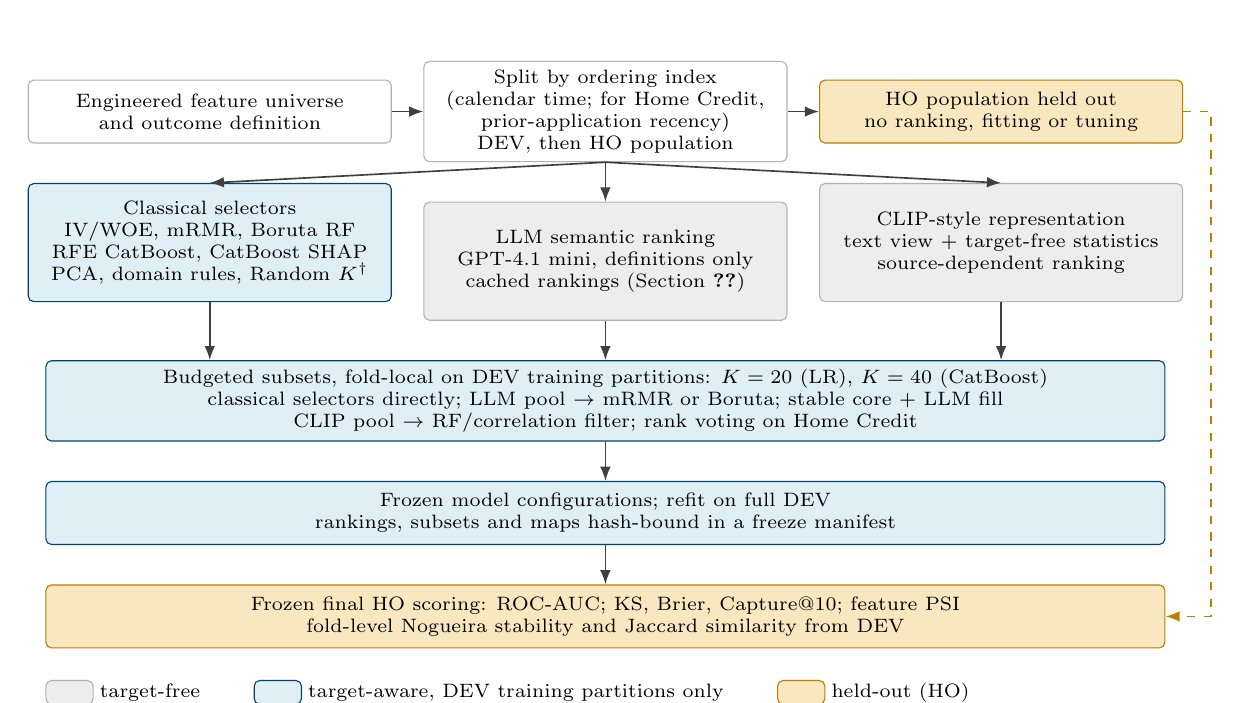
\begin{tikzpicture}[
    font=\scriptsize,
    box/.style={draw=gray!60, rounded corners=2pt, align=flush center, inner sep=3pt, minimum height=8mm, fill=white},
    tfree/.style={box, fill=gray!14},
    taware/.style={box, fill=cBlue!12, draw=cBlue!60!black},
    oot/.style={box, fill=cOrange!25, draw=cOrange!80!black},
    arr/.style={-{Latex[length=1.8mm]}, semithick, gray!50!black},
    darr/.style={-{Latex[length=1.8mm]}, semithick, dashed, cOrange!80!black},
    node distance=5mm and 4mm
]
\node[box, text width=44mm] (data) {Engineered feature universe\\and outcome definition};
\node[box, text width=44mm, right=of data] (split) {Split by ordering index\\(calendar time; for Home Credit,\\prior-application recency)\\DEV, then HO population};
\node[oot, text width=44mm, right=of split] (ootheld) {HO population held out\\no ranking, fitting or tuning};

\node[taware, text width=44mm, minimum height=15mm, below=of data] (classical) {Classical selectors\\IV/WOE, mRMR, Boruta RF\\RFE CatBoost, CatBoost SHAP\\PCA, domain rules, Random $\Kfeat^{\dagger}$};
\node[tfree, text width=44mm, minimum height=15mm, below=of split] (llm) {LLM semantic ranking\\GPT-4.1 mini, definitions only\\cached rankings (Section~\ref{subsec:llm_fs})};
\node[tfree, text width=44mm, minimum height=15mm, below=of ootheld] (clip) {CLIP-style representation\\text view + target-free statistics\\source-dependent ranking};

\node[taware, text width=140mm, below=of llm] (subset) {Budgeted subsets, fold-local on DEV training partitions: $\Kfeat=20$ (LR), $\Kfeat=40$ (CatBoost)\\classical selectors directly; LLM pool $\rightarrow$ mRMR or Boruta; stable core + LLM fill\\CLIP pool $\rightarrow$ RF/correlation filter; rank voting on Home Credit};
\node[taware, text width=140mm, below=of subset] (model) {Frozen model configurations; refit on full DEV\\rankings, subsets and maps hash-bound in a freeze manifest};
\node[oot, text width=140mm, below=of model] (eval) {Frozen final HO scoring: ROC-AUC; KS, Brier, Capture@10; feature PSI\\fold-level Nogueira stability and Jaccard similarity from DEV};

\draw[arr] (data) -- (split);
\draw[arr] (split) -- (ootheld);
\draw[arr] (split) -- (llm);
\draw[arr] (split.south) -- (classical.north);
\draw[arr] (split.south) -- (clip.north);
\draw[arr] (classical) -- (classical.south |- subset.north);
\draw[arr] (llm) -- (subset);
\draw[arr] (clip) -- (clip.south |- subset.north);
\draw[arr] (subset) -- (model);
\draw[arr] (model) -- (eval);
\draw[darr] (ootheld.east) -- ++(3.5mm,0) |- (eval.east);

\node[tfree, minimum height=3mm, minimum width=6mm, inner sep=0pt, anchor=north west] (l1) at ([yshift=-4mm]eval.south west) {};
\node[anchor=west, inner sep=2pt] (t1) at (l1.east) {target-free};
\node[taware, minimum height=3mm, minimum width=6mm, inner sep=0pt, anchor=west] (l2) at ([xshift=6mm]t1.east) {};
\node[anchor=west, inner sep=2pt] (t2) at (l2.east) {target-aware, DEV training partitions only};
\node[oot, minimum height=3mm, minimum width=6mm, inner sep=0pt, anchor=west] (l3) at ([xshift=6mm]t2.east) {};
\node[anchor=west, inner sep=2pt] at (l3.east) {held-out (HO)};
\end{tikzpicture}
\caption{Research pipeline. Grey boxes are target-free stages that consume metadata and development statistics only (the contrastive scoring is target-free conditional on its frozen source anchor, \ref{app:clip}); blue boxes are target-aware stages confined to DEV training partitions and refitted once on full DEV, except that PCA, domain rules and Random $\Kfeat$ ($\dagger$), grouped with the classical selectors, are themselves target-free (Table~\ref{tab:methods}); orange boxes concern the held-out population (HO), which the frozen final pipelines score once; the HO populations were inspected in earlier protocol versions (Section~\ref{subsec:protocol_development}), so this is a frozen final scoring run, not a first look. The ordering index of the split is calendar time for LendingClub and Stability 2024 and prior-application recency for Home Credit.}
\label{fig:pipeline}
\end{figure*}

\subsection{Data Preprocessing}
\label{subsec:preprocessing}

Numeric variables are processed by replacing infinite values with missing values, imputing with the training-partition mean and standardising with training-partition statistics. Categorical variables receive an explicit missing token and are one-hot encoded; levels unseen in the training partition are ignored, and rare levels are dropped below a minimum frequency of 10 observations for Home Credit and Stability 2024 and 50 for LendingClub. The order of operations is fixed: eligibility screening and selection operate on \emph{original} features, one column per candidate, so a categorical variable is selected or rejected as a whole, and one-hot expansion is performed only after the subset has been selected, so that the budget $\Kfeat$ counts original variables. Principal-component selection is the one exception, since its retained quantities are components. Preprocessing maps are fitted on the training partition of each fold and, for the final model, on full DEV.

\subsection{Classical Feature-Selection Methods}
\label{subsec:classical_fs}

Table~\ref{tab:methods} lists the fourteen strategies and the full-feature reference. All target-aware selectors are fitted on the training partition of each fold with DEV labels only and refitted on full DEV before HO scoring; unless stated otherwise, candidates are ranked by the method's own criterion and the top $\Kfeat$ original features are kept. \emph{IV/WOE} ranks by Eq.~\eqref{eq:iv} computed on the training partition with ten quantile bins \cite{siddiqi2006}, and the same statistic defines the pre-screen of \emph{IV then Boruta}. \emph{mRMR} applies Eq.~\eqref{eq:mrmr} with mutual information estimated on the training partition \cite{peng2005,kraskov2004,ross2014}; its pool is the whole candidate set when it is used alone and the shortlist when it follows a semantic stage. Throughout the paper \emph{mRMR} denotes this mutual-information implementation; the random-forest/correlation rule used inside the contrastive branch is called the \emph{RF/correlation filter} (\ref{app:clip}) and was named legacy mRMR in the early versions of the study. \emph{Boruta RF} confirms features whose random-forest importance (500 trees of depth 6) exceeds the best shuffled shadow importance at $\alpha=0.05$ with two-step correction and keeps the top $\Kfeat$ confirmed features \cite{kursa2010,breiman2001}. When fewer than $\Kfeat$ features are confirmed, the subset consists of the confirmed features alone and is flagged as below budget; tentative or rejected features are never added. \emph{RFE CatBoost} removes 20\% of the surviving features per step by the importance of an internal CatBoost ranker (500 iterations, depth 6, learning rate 0.05) until $\Kfeat$ remain \cite{guyon2002}. \emph{CatBoost SHAP} keeps the $\Kfeat$ features with the largest aggregate absolute SHAP contribution over a 10,000-row training sample \cite{lundberg2017}. \emph{PCA} retains the leading components and is reported as a transformation baseline \cite{jolliffe2016}. \emph{Domain rules} is a deterministic credit-domain scorer that reads no data and calls no model: 42 named-variable rules, family and string-pattern rules for bureau, instalment, credit-card and previous-application aggregates, 15 property-attribute rules and nine semantic-group fallbacks assign each feature a priority, which aggregation suffixes and leakage status adjust, with deterministic tie ordering. The five Home Credit features its leakage rules flag, the aggregates of the count of future instalments in the point-of-sale record, all fail the missingness screen and lie outside the 373-feature candidate set, so no selector could have chosen them. Remaining implementation details are fixed in the public code repository.

\begin{table*}[htbp]
\centering
\footnotesize
\begin{threeparttable}
\caption{Feature-selection strategies evaluated. ``Labels'' states whether the stage that produces the final subset uses DEV outcomes; ``Datasets'' states where the strategy is evaluated on held-out data. The full-feature model is a reference and is excluded from selector comparisons.}
\label{tab:methods}
\begin{tabular}{@{}llL{46mm}cl@{}}
\toprule
Method & Family & Selection role & Labels & Datasets \\
\midrule
Full features & Reference & No selection; context only & -- & All three \\
Domain rules & Classical & Eligibility and policy filters from credit-domain definitions & no & All three \\
Random $\Kfeat$ & Baseline & Uniformly random subset of size $\Kfeat$; the floor for every selector & no & All three \\
PCA & Classical & Leading components of the standardised candidates (components, not original features) & no & All three \\
IV/WOE & Classical & Ranking by information value, Eq.~\eqref{eq:iv} & yes & All three \\
mRMR & Classical & Mutual-information relevance against mutual-information redundancy, Eq.~\eqref{eq:mrmr} & yes & All three \\
Boruta RF & Classical & All-relevant random-forest wrapper with shadow-feature comparison & yes & All three \\
IV then Boruta & Classical hybrid & IV eligibility screen followed by Boruta confirmation & yes & All three \\
RFE CatBoost & Model wrapper & Recursive elimination driven by CatBoost importance & yes & All three \\
CatBoost SHAP & Embedded & Ranking by aggregated absolute SHAP contribution & yes & All three \\
Pure LLM & LLM-assisted & Top-$\Kfeat$ names of the cached semantic ranking of the fold & no & All three \\
LLM then mRMR & LLM hybrid & Semantic pool of 60 (LR) or 100 (CatBoost), then mRMR & yes & All three \\
LLM then Boruta & LLM hybrid & Semantic pool, then Boruta confirmation & yes & All three \\
Stable core + LLM fill & LLM hybrid & Bootstrap-stable RF/correlation core completed from the LLM ranking & yes & All three \\
CLIP-ranked & Representation & Contrastive ranking, target-free given its frozen anchor, then RF/correlation filter (supplementary, \ref{app:clip}) & yes & Stability 2024\tnote{a} \\
\bottomrule
\end{tabular}
\begin{tablenotes}\footnotesize
\item[a] Held-out results on Stability 2024 only (\ref{app:clip}); the Home Credit experiments of earlier protocol versions are summarised in Table~\ref{tab:stages}. The rank-voting experiment of \ref{app:voting} covers Home Credit, and its classical voting family Home Credit and LendingClub.
\end{tablenotes}
\end{threeparttable}
\end{table*}

\subsection{Pure LLM Selection}
\label{subsec:llm_fs}

The language model is GPT-4.1 mini \cite{openai2025gpt41}, snapshot \path{gpt-4.1-mini-2025-04-14}, called through the Chat Completions interface with temperature 0 and a JSON response format; it never receives rows, outcomes, validation statistics or HO information. One prompt template, reproduced verbatim in \ref{app:prompts}, is used for all three datasets under a single \emph{definition-only} information contract. The template carries an evidence-mode placeholder with two admissible values, \texttt{definitions\_only} and \texttt{training\_metadata}; every call in this study used \texttt{definitions\_only}, under which the model may use feature names, definitions, source lineage, aggregation operations and observation windows and no numerical summary of any kind, so missingness, moments, quantiles and cardinalities are withheld as well as every target-conditioned statistic, and the prompt forbids drawing on remembered dataset-specific results. For each candidate the record supplied carries the feature name, its description, source family, lineage formula and semantic group, with the aggregation operation and window of an engineered feature stated in the formula and the name. The descriptions are prepared before ranking from the source-variable definitions, with the aggregation operation and time window of an engineered feature stated in words (Section~\ref{subsec:protocol_development}). 

A ranking-budget placeholder fixes the number of names requested, and the prompt asks for exactly that many distinct features ordered from highest to lowest priority, to be refined downstream by the documented budgets. It directs the model to exclude only features whose supplied definition or lineage reveals the outcome, post-decision information or the evaluation split, and to weigh uncertain timing as a concern rather than as leakage. It asks for durable credit meaning, broad semantic coverage and decision-time availability, for avoidance of near-duplicate aggregates of one concept while leaving correlation-based pruning to the statistical selectors, and for alphabetical resolution of remaining ties. When fewer eligible candidates than the budget remain, the model must return status \texttt{error} with an empty list rather than a shortened or padded list. Responses are validated strictly: every name must appear verbatim among the candidate records and the array must contain exactly the requested number of distinct names; a failing response is re-requested up to three times and no fallback ranking is used. 

The ranking is requested separately for each of the five fold training partitions and for full DEV, and the candidate records supplied are those of the partition. On Home Credit the candidate list is the same 373 of the 529 features in every call, fixed by the missingness screen on the earliest training fold; on LendingClub it is all 675 features, none of which fails the screen; on Stability 2024 it is the 1,068 eligible features (Table~\ref{tab:datasets}). On Home Credit six rankings of 100 names were obtained, one per partition, and the budgets of 20, 40, 60 and 100 are their prefixes; on LendingClub a separate call was made for each budget of 20, 40, 60 and 100 names, giving 24 cached rankings; on Stability 2024 one ranking of 100 names was obtained in a single call, accepted at the first attempt. Each response is validated as above, cached and hash-bound, and the cached response rather than a fresh call is the reproducible artefact: the cached orderings all differ from one another, and calls with identical prompt, model and temperature returned different lists, so a fixed model identifier and zero temperature do not guarantee identical outputs (Section~\ref{subsec:stability_results}). The \emph{pure LLM} selector retains the top $\Kfeat$ names of the ranking of its partition and budget. Three call structures were therefore used: per-partition calls with a budget of 100 on Home Credit, per-partition and per-budget calls on LendingClub, and a single call on Stability 2024. The token and cost figures of Section~\ref{subsec:cost_runtime} cover Home Credit and LendingClub only, because the usage of the Stability 2024 call was not recorded.

To test whether the ranking depends on recognising feature names, the six Home Credit calls were repeated in two obfuscated arms with everything except the feature records held fixed: the same snapshot (\texttt{gpt-4.1-mini-2025-04-14}), temperature 0, JSON response format, the template of \ref{app:prompts}, the definition-only evidence mode, the same 373 candidates per partition and the same strict validation. In arm A every name was replaced by an identifier \texttt{F001}--\texttt{F529} drawn from a seeded permutation (seed 20260914) of the universe, the permutation being drawn per partition so that no identifier carries meaning across calls, and every literal occurrence of the original name was removed from the description text as well; the model saw only identifiers and descriptions, and the identifier-to-name table never entered a prompt. In arm B the names were kept and the descriptions were blank. Each arm yields six rankings of 100 identifiers, decoded and carried through the frozen downstream pipeline exactly as the named rankings are: top 20 to logistic regression and top 40 to CatBoost, five fold models plus the full-DEV refit with the fixed configurations of Section~\ref{subsec:models} (seed 42), scored on the same 120,053 HO rows. The outcome is reported in Section~\ref{subsec:obfuscation_results}.

\subsection{Hybrid Selection Methods}
\label{subsec:hybrid_fs}

Three hybrids combine the cached semantic ranking with target-aware refinement. \emph{LLM then mRMR} takes the top 60 (logistic regression) or top 100 (CatBoost) features of the ranking as the pool and applies mutual-information mRMR on the fold training partition to reach $\Kfeat$. The semantic stage is intended to remove variables an analyst would consider implausible or redundant in meaning, and the statistical stage variables redundant in the data; on Home Credit, however, the statistical selector applied to the whole candidate set attained a higher HO AUC than every pipeline that applied mRMR to a semantic pool (\ref{app:voting}). \emph{LLM then Boruta} applies Boruta confirmation to the same pool and truncates to the budget. \emph{Stable core + LLM fill} draws five bootstrap resamples of the fold training partition (80\% with replacement, seeds 42 to 46) and runs the RF/correlation filter on each. Features selected in at least four of the five resamples form the stable core, ordered by selection frequency and mean rank; the subset is then completed from the LLM ranking in rank order, without padding from unranked features, so that the core preserves reproducibility while semantically prioritised variables fill the remaining budget. None of these pipelines is target-free as a whole, and the fold-to-fold stability of a hybrid subset depends on both the per-fold semantic ranking and the fitted target-aware stage.

\subsection{Development of the Protocol}
\label{subsec:protocol_development}

The protocol above is the final form of an evaluation developed through successive versions, and the final results supersede the earlier ones. Table~\ref{tab:stages} records the changes that mattered and their consequences. Each version froze its pipelines before scoring its held-out population, but later versions were designed with knowledge of the held-out results of earlier ones, so the final evaluation is a frozen scoring run on held-out populations that had been inspected in earlier versions. The DEV/HO design of Home Credit and LendingClub was fixed from the outset, and the Stability 2024 cutoff was moved once, from 2020-02-26 to 2020-02-01, for the final evaluation (Section~\ref{subsec:dev_oot}). What changed otherwise was the comparator set, the semantic inputs of the LLM stage, the statistical selector used as the classical reference, the inference procedure, and the correctness of the reported values.

Three changes coincided with changes in the numbers. First, the comparator changed from a single mRMR baseline on two datasets to the classical selector with the highest observed HO AUC in each case, drawn from the full selector set on three datasets; the LLM-assisted comparator is chosen in the same way, and this selection of both headline methods on the HO results is why the headline comparisons of Table~\ref{tab:primary_results} are descriptive (Section~\ref{subsec:inference}). The development-data rule of Table~\ref{tab:confirmatory}, which chooses each family's leader on the mean DEV fold AUC, was specified after these HO-rule results were known; it uses no HO information, and both rules are reported. Second, the way feature descriptions are prepared for the language model was revised. In the early versions semantic explanations were written after feature selection; in the revised process the descriptions are prepared before LLM ranking, starting from the source-variable definition and stating the aggregation operation and time window in words, so that, for example, the mean of a bureau annuity amount over the records of a case is described as the average bureau annuity amount of the case. The revision was intended to give the language model accurate meanings for the engineered features. It is a substantive protocol change that coincides with the difference between the LLM-related scores of the early versions and of the final tables; its isolated effect was not established, because the reported comparisons also changed comparators, selectors and datasets. Third, the mutual-information mRMR of the final protocol replaced the RF/correlation filter of the early versions as the stand-alone statistical selector, which is why the Home Credit logistic-regression mRMR reference of the final tables (0.7699) differs from the earlier value (0.7457).

Two inference changes altered what could be claimed rather than the estimates. Five-fold rank tests, whose minimum attainable two-sided $p$-value with five non-zero pairs is 0.0625, gave way to paired inference on matched HO observations, and the six headline comparisons were reported with paired bootstrap confidence intervals and without significance claims, because the identities of the compared methods had been determined from the HO results. Finally, earlier report versions contained transcription and rounding errors that the final revision corrected. Earlier values are therefore superseded and are quoted only where the text says so.

\begin{table*}[htbp]
\centering
\footnotesize
\setlength{\tabcolsep}{5pt}
\begin{threeparttable}
\caption{Protocol versions and the final evaluation. Values quoted in the last column for the superseded versions were computed with earlier comparator sets, earlier semantic inputs and, in the earliest versions, the RF/correlation filter as the mRMR reference; the last row is the evaluation reported in this paper.}
\label{tab:stages}
\begin{tabular}{@{}L{27mm}L{\dimexpr(\textwidth-27mm-4\tabcolsep)/2\relax}L{\dimexpr(\textwidth-27mm-4\tabcolsep)/2\relax}@{}}
\toprule
Protocol version & Change to the methodology & Effect on the results, and why (superseded values) \\
\midrule
Home Credit comparison & 16 pipelines on the 373 screened features; the LLM produces a top-100 pool refined by mRMR, Boruta or a stable-core rule; six LLM calls reused across pipelines. & Best HO AUC from CatBoost with LLM then mRMR (0.772 against 0.769 for mRMR). A variant whose LLM shortlist was almost as small as the budget gave no gain, so the LLM was fixed as a broad first-pass screener rather than the final selector. \\
\addlinespace
Corrected contrastive representation & Identity-equivalence pairing policy; incremental evaluation of the representation after LLM screening; bidirectional transfer diagnostics with LendingClub as source. & HO AUC changed by less than 0.002 while fold Jaccard rose by 0.32 to 0.50; the contrastive branch was assigned to reproducibility and portability rather than discrimination. \\
\addlinespace
Two-dataset canonical comparison & Home Credit and LendingClub, four selectors, 16 runs; five-fold exact Wilcoxon tests; type-aware feature PSI repaired for 480 selected-feature occurrences; usage and cost accounting. & No fold test could reach $p<0.05$ (minimum attainable 0.0625), so fold tests were abandoned as underpowered; pure LLM had lower feature drift in three of four cells; direct API cost bounded at USD 0.171 to 0.413. \\
\addlinespace
Matched HO inference and voting & Paired DeLong tests and 2,000-resample paired bootstrap on matched observation identifiers, Holm correction within families; eight voting variants added. & 11 of 12 canonical differences became significant, with dataset-dependent signs; voting exceeded sequential screening in 5 of 8 variants and full-pool mRMR in none. \\
\addlinespace
Three-dataset evaluation & Stability 2024 added (HO cutoff 2020-02-26); fourteen selectors and a full-feature reference; revised semantic representation of the features supplied to the LLM; three-source contrastive extension; per-case classical family leader as comparator. & LLM-assisted led five of six AUC cases at the point-estimate level; CLIP subset reproducibility and source-dependent transfer established; the family-leader comparator lowered the apparent LLM advantage relative to the two-dataset comparison, while the revised feature descriptions coincided with higher LLM-related scores. \\
\addlinespace
Cross-dataset classical voting & Pre-declared family of twelve comparisons on Home Credit and LendingClub: three classical voters (RF/correlation mRMR, Boruta, RFE), pools of 100, 200 and 300, RF/correlation mRMR reference on the candidate set. & All twelve differences positive and Holm-significant, from $+0.0020$ to $+0.0129$ AUC (\ref{subsec:voting_results}). \\
\addlinespace
Final revised evaluation (this paper) & Stability 2024 HO cutoff moved from 2020-02-26 to 2020-02-01 to balance event rates (3.16\% DEV, 3.09\% HO); six paired comparisons between HO-chosen family leaders with bootstrap confidence intervals, reported descriptively, and six development-rule comparisons between DEV-chosen leaders with Holm-adjusted paired DeLong tests; exact AUC precision; mutual-information mRMR distinguished from the RF/correlation filter; transcription and rounding errors of earlier versions corrected. & Results of Section~\ref{sec:results}; the contrastive extension was not re-run and remains on the 2020-02-26 cohort, so it is compared with the headline selectors descriptively only. \\
\bottomrule
\end{tabular}
\end{threeparttable}
\end{table*}

% ============================================================
% 5. EXPERIMENTAL SETUP
% ============================================================

\section{Experimental Setup}
\label{sec:experimental_setup}

\subsection{Datasets}
\label{subsec:datasets}

Three public credit datasets released through Kaggle are used (Table~\ref{tab:datasets}). \emph{Home Credit} is the Home Credit Default Risk data \cite{homecredit2018}: the unit is a loan application, the event is the provider's binary target (payment difficulties), and the universe contains 529 original features derived from the application record and the auxiliary tables. Its ordering index is \texttt{DAYS\_DECISION}, the number of days between the applicant's most recent previous application and the current application, so the split is a recency-based covariate-shift holdout rather than a calendar-time split of the current applications. DEV holds applicants whose most recent previous application is 241 to 600 days old and HO those with a more recent one. Features that are functions of this index, the previous-application decision days and their aggregates, are not in the candidate set of any selector, so no selector could learn on a range of the index that HO does not contain. Applications without a previous application within the 600-day window, about 29\% of the 307,511 applications in the public release, are excluded, which limits the population to which the Home Credit results apply. Every selector, classical and LLM-assisted, selects from the 373 features that pass the 90\% missingness screen on the earliest training fold; the budget of 20 or 40 features is the same for all.

\emph{LendingClub v2} is the LendingClub loan book \cite{lendingclub_kaggle}: only resolved 36- and 60-month loans through the 2019-05-01 snapshot are retained, with charged-off or defaulted loans as events and fully paid loans as non-events. The 675 features were generated deterministically from roughly 93 distinct columns of the loan book, and every one of them is an attribute of a single loan and its applicant at origination: 116 raw columns carried through unchanged, 180 binary flags, 158 ratios, 88 missing indicators, 78 further engineered variables, 27 binned versions, 19 interactions and 9 categoricals. No feature aggregates across loans or over calendar periods, and the only elapsed-time quantity is the age of the credit file at issue, the number of months between \texttt{issue\_d} and \texttt{earliest\_cr\_line}, which is an attribute of the loan rather than a time index. A prediction-time availability review removed two groups of source columns before any feature was built. The first is every post-origination field, among them \texttt{total\_pymnt}, \texttt{recoveries}, \texttt{last\_pymnt\_amnt}, \texttt{out\_prncp}, the \texttt{last\_fico\_range} fields, \texttt{hardship\_flag} and \texttt{debt\_settlement\_flag}, which record what happened after the credit decision and would reveal the outcome. The second is LendingClub's own pricing and grading fields, \texttt{int\_rate}, \texttt{grade}, \texttt{sub\_grade}, \texttt{installment} and \texttt{funded\_amnt}, which encode the platform's own assessment of the application: excluding them poses the selection problem over applicant and bureau attributes rather than over a re-encoding of a credit decision already taken, at the cost that the AUC levels reported here are not comparable with LendingClub studies that retain the platform's grade or interest rate. Several credit-file attributes of the loan book were introduced by the platform during the sample period, so their missingness is higher in DEV than in HO, and the features derived from them inherit that pattern; the highest missingness rate reached by any LendingClub feature on the earliest training partition is 82\%, so the screen that defines the candidate set retains all 675; 566 features fall below 40\%, two lie between 40 and 60\% and 107 between 60 and 82\%. None of them appears anywhere in the cached semantic rankings, so no LLM-assisted subset contains one; the target-aware selectors compute their criteria on the DEV training partition, where a field that is sparse in that period carries little information value, mutual information or model importance and is down-weighted by construction. Both the language model and the classical selectors select from the same 675 features. The ordering index is the number of days from the issue month to the last finalised issue month, 2018-12-01, so the HO window is later in calendar time. DEV comprises the loans issued from January 2014 to December 2015 and HO the loans issued in 2016. Thirty-six-month loans account for 445,596 of the 598,649 DEV loans and 232,361 of the 293,105 HO loans, with event rates of 14.5\% (36-month) and 34.3\% (60-month) in DEV and 19.8\% and 36.4\% in HO, so the DEV--HO difference in event rate arises within both terms and not only from a change in term mix.

\emph{Stability 2024} is the Home Credit Credit Risk Model Stability data \cite{homecredit2024}: the unit is a credit decision dated by \texttt{date\_decision} and the event is the provider's default target. The 1,959 engineered features were generated deterministically from the 434 approved raw predictors. The training base table defines the population and the case identifier. At depth 0 the two static families, \texttt{static\_0} and \texttt{static\_cb\_0}, are joined one-to-one to the base. At depth 1 ten table families with several rows per case, \texttt{applprev\_1}, \texttt{tax\_registry\_a\_1}, \texttt{tax\_registry\_b\_1}, \texttt{tax\_registry\_c\_1}, \texttt{credit\_bureau\_a\_1}, \texttt{credit\_bureau\_b\_1}, \texttt{other\_1}, \texttt{person\_1}, \texttt{deposit\_1} and \texttt{debitcard\_1}, are reduced to one row per case with fixed outcome-independent operations: count, mean, minimum, maximum, standard deviation and the chronologically latest value for numeric and date variables, and mode, most recent category and number of distinct values for categorical variables. Date variables are expressed relative to \texttt{date\_decision} where appropriate and future information is excluded; depth-2 tables are excluded; no ratios, interactions or target-informed transformations are introduced; and every generated variable keeps its lineage to the raw table, raw variable, depth, operation and type rule. Time windows, where they appear, come from the names of the raw predictors rather than from the engineering. Of the 1,959 features, the 1,068 with at most 90\% missing values on the earliest training fold form the LLM candidate set. Home Credit and Stability 2024 share institutional lineage, whereas LendingClub is a distinct peer-to-peer platform, which matters for the transfer experiments.

\begin{table*}[htbp]
\centering
\footnotesize
\begin{threeparttable}
\caption{Datasets, held-out partitions and feature universes. The candidate set is the screened universe from which every selector chooses, fixed on the earliest training fold. HO labels the held-out population of each dataset. Home Credit windows are days of the most recent previous-application decision relative to the current application, a recency-based covariate-shift holdout rather than a calendar-time split; LendingClub windows are days from the issue month to 2018-12-01; Stability 2024 windows are calendar dates of \texttt{date\_decision}.}
\label{tab:datasets}
\begin{tabular}{@{}lL{29mm}L{31mm}L{31mm}@{}}
\toprule
 & Home Credit & LendingClub v2 & Stability 2024 \\
\midrule
Observation unit & Loan application & Issued loan & Credit decision \\
Event definition & Payment difficulties (provider target) & Charged off or default; resolved loans only & Default (provider target) \\
DEV window & day $-600$ to $-241$ & day $-1795$ to $-1096$ (issued 2014-01 to 2015-12) & 2019-01-01 to 2020-01-31 \\
DEV $N$ & 99,092 & 598,649 & 1,157,512 \\
DEV event rate & 7.93\% & 19.54\% & 3.16\% \\
HO window & day $-240$ to $-1$ & day $-1065$ to $-730$ (issued 2016-01 to 2016-12) & 2020-02-01 to 2020-10-05 \\
HO $N$ & 120,053 & 293,105 & 369,147 \\
HO event rate & 8.90\% & 23.29\% & 3.09\% \\
Feature universe & 529 original features & 675 engineered features (93 source columns) & 1,959 engineered features \\
Candidate set, all selectors & 373 of 529 ($\le$90\% missing) & 675 of 675 ($\le$90\% missing) & 1,068 of 1,959 ($\le$90\% missing) \\
\bottomrule
\end{tabular}
\begin{tablenotes}\footnotesize
\item The Stability 2024 column describes the cohort of the headline evaluation (cutoff 2020-02-01). The contrastive extension (Table~\ref{tab:clip_cells}) uses the earlier cohort: DEV 2019-01-01 to 2020-02-25 (1,221,743 decisions, 3.24\%), HO 2020-02-26 to 2020-10-05 (304,916 decisions, 8,349 events, 2.74\%).
\end{tablenotes}
\end{threeparttable}
\end{table*}

\subsection{Held-Out DEV/HO Design}
\label{subsec:dev_oot}

Each dataset is partitioned along its ordering index into a development population (DEV) and a held-out population (HO). For LendingClub and Stability 2024 the index is calendar time and HO is later than DEV, which addresses whether a selected subset and a fitted model still rank risk correctly on loans issued or decisions taken after development; random splits would mask both population drift and the optimism of subsets tuned on the same period \cite{bergmeir2012,gama2014}. The split orders decisions, not outcomes: the provider-defined outcome horizons are not fully specified (Section~\ref{subsec:limitations}), so the design is a chronological holdout and does not by itself establish that every development label would have been observable at the held-out decision dates, as a fully simulated deployment would require. For Home Credit the index is prior-application recency, so HO is a recency-based covariate-shift holdout of applicants with a more recent previous application, not a set of later applications. The split point was fixed on the index rather than on a target share of the population, so the Home Credit HO population (120,053 applications drawn from a 240-day recency window) is larger than DEV (99,092 from a 360-day window): applicants whose most recent previous application is recent are denser in the release than those whose most recent one is old. The ordering constraint was preferred to an equal split because moving the cut to balance the two sides would have set it with knowledge of the population it defines. Within DEV, five expanding-window folds are formed along the same index, each training partition consisting of the lowest-index observations and the validation partition of a later block, separated by a gap of one index group, one index day for Home Credit and LendingClub and one decision date for Stability 2024. The gap is one unit of each dataset's own index and is not a calendar embargo: LendingClub is indexed by issue month, so a one-day gap there separates the partitions by position in the ordering and not by elapsed time, and it is the ordered split itself rather than the gap that keeps later loans out of training. For Home Credit these folds are ordered by recency rather than by application date, so the expanding window enlarges the training partition along the recency index for consistency with the other two datasets rather than to simulate the passage of time. Every component is fitted on the training partition, applied to the validation partition without refitting, and refitted once on full DEV after development.

For Stability 2024 the HO cutoff of the headline evaluation is 2020-02-01: DEV comprises the 1,157,512 decisions dated 2019-01-01 to 2020-01-31 (event rate 3.16\%) and HO the 369,147 decisions dated 2020-02-01 to 2020-10-05 (3.09\%), 24.2\% of the 1,526,659 decisions. During protocol development the cutoff was 2020-02-26 (DEV 1,221,743 decisions at 3.24\%; HO 304,916 decisions with 8,349 events, 2.74\%). It was moved 25 days earlier for the final evaluation, after the earlier run had been scored, because the later tail compared the development population with a materially lower-risk HO population. The contrastive extension of \ref{app:clip} was not re-run and is reported on the 2020-02-26 cohort; it is not scored on the same HO population as the headline comparisons and is compared with them descriptively only. The LendingClub HO window runs from day $-1065$ to day $-730$ (loans issued from 2016-01 through 2016-12), and only loans resolved by the 2019-05-01 snapshot are evaluated; loans unresolved at the snapshot are excluded. This restriction can preferentially retain early defaults and early repayments when other loans of the same cohort remain unresolved, and follow-up duration differs across issue cohorts and between 36- and 60-month terms, so population composition and the reported DEV--HO event-rate difference (Table~\ref{tab:datasets}) should be read with this selection in mind, and the LendingClub findings describe this resolved-loan population. Before each final scoring run, the feature universe, the cached LLM rankings, the contrastive representations and rankings, every selected subset, the preprocessing maps, and the model configurations and fitted models are frozen, and HO rows enter only the computation of the reported metrics. The Stability 2024 event rates informed the cutoff described above (Section~\ref{subsec:protocol_development}).

\subsection{Predictive Models}
\label{subsec:models}

Two backbones are used in every dataset--selector case, spanning a linear scorecard-style model and a non-linear boosted model \cite{lessmann2015,gunnarsson2021}, with configurations fixed and identical across selectors. The logistic regression uses the \texttt{liblinear} solver of scikit-learn \cite{pedregosa2011} with an L2 penalty and $C=1$, at most 1,000 iterations, balanced class weights and random seed 42. CatBoost \cite{prokhorenkova2018} uses depth 10, learning rate 0.01, L2 leaf regularisation 95, minimum 290 observations per leaf, a feature-sampling rate (\texttt{rsm}) of 0.90, random strength 0.125, depthwise growth, Bernoulli bootstrap with subsample 0.55, the Logloss objective with AUC evaluation, balanced class weights, seed 42, four threads and a fixed 1,500 iterations without early stopping, so that no validation information enters the fitted model. Balanced class weights are used because event rates range from about 3\% to 23\%. The same two configurations are applied to every feature count, from the 20- and 40-feature subsets to the full-feature reference models on 373, 675 and 1,959 features, the Stability 2024 references being fitted on the unscreened 1,959-feature universe; the CatBoost configuration was carried over unchanged from the authors' prior credit-scoring work at the Central Bank of the Republic of Uzbekistan on a separate, non-public portfolio, where it had been tuned on a validation set, and the logistic-regression configuration is a standard L2-penalised setting with $C=1$. No hyperparameter of either backbone was tuned on any partition of the three datasets studied here, and one configuration per backbone serves all three. The full-feature reference was not tuned separately, so the ``Full'' column of Table~\ref{tab:primary_results} is a context model under the compact configuration, not a tuned upper bound for the full universe.

\subsection{Feature Budgets}
\label{subsec:feature_budgets}

The budgets are $\Kfeat=20$ original features for logistic regression and $\Kfeat=40$ for CatBoost. They were determined in DEV-only experimentation and frozen before HO evaluation. Larger linear subsets improved development discrimination only marginally, on average $+0.004$ development AUC at $\Kfeat=30$ and $+0.005$ at $\Kfeat=40$ for one and a half to two times the feature count, so $\Kfeat=20$ was fixed as the compact operating point; CatBoost continued to benefit up to $\Kfeat=40$, gained nothing further beyond it on average, and was less sensitive to redundant predictors. \ref{app:budgets} reports the development curves and shows that the budget sets the level of every selector in a case without changing the ordering between the two families. The budgets are model-specific rather than dataset-specific, so selectors within a backbone are compared at equal subset size, whereas comparisons between backbones differ in both model class and budget.

\subsection{Evaluation Metrics}
\label{subsec:metrics}

Let $y_i\in\{0,1\}$ be the event label of HO observation $i$, $p_i$ its predicted event probability, $N_+$ and $N_-$ the numbers of events and non-events, and $N=N_++N_-$.

\paragraph{ROC-AUC}
The area under the receiver operating characteristic curve is the probability that a randomly chosen event scores higher than a randomly chosen non-event, with half credit for ties \cite{hanley1982},
\begin{equation}
    \AUC=\frac{1}{N_+N_-}\sum_{i:\,y_i=1}\sum_{j:\,y_j=0}\big[\mathbf{1}(p_i>p_j)+\tfrac12\mathbf{1}(p_i=p_j)\big].
    \label{eq:roc_auc}
\end{equation}
Higher is better. ROC-AUC is threshold-free and is the sole headline metric; the Gini coefficient $2\,\AUC-1$ adds no information.

\paragraph{KS}
The Kolmogorov--Smirnov statistic is the maximum vertical separation between the cumulative score distributions of events and non-events,
\begin{equation}
    \KS=\max_{t}\,\big[\TPR(t)-\FPR(t)\big],
    \label{eq:ks}
\end{equation}
which equals the maximum Youden index over thresholds \cite{youden1950}; higher is better. KS is reported as the maximum HO separation. A KS-optimal operating threshold is also recorded in each freeze manifest for deployment, but no threshold-dependent metric is reported, so the threshold plays no part in the results.

\paragraph{Brier score}
The Brier score is the mean squared error of the predicted probabilities \cite{brier1950},
\begin{equation}
    \mathrm{Brier}=\frac{1}{N}\sum_{i=1}^{N}(y_i-p_i)^2 ,
    \label{eq:brier}
\end{equation}
lower is better. It measures the overall squared error of the predicted probabilities, which combines calibration and resolution, rather than ranking; a constant prediction equal to the event rate $\pi$ attains $\pi(1-\pi)$, and log loss, $-N^{-1}\sum_i[y_i\ln p_i+(1-y_i)\ln(1-p_i)]$, is a supporting diagnostic. Because both backbones use balanced class weights and no recalibration (Section~\ref{subsec:models}), their outputs are not population event probabilities, so Brier values compare selectors within a dataset and do not indicate deployment-ready calibration.

\paragraph{Capture@10 and Lift@10}
Let $T$ be the set of observations in the highest-scored decile, a fraction $q=|T|/N\approx0.10$ of the population. Capture@10 is the share of all events found in that decile and Lift@10 the ratio of the decile event rate to the portfolio event rate,
\begin{equation}
\begin{aligned}
    \mathrm{Capture@10}&=\frac{\sum_{i\in T}y_i}{\sum_{i}y_i},\\
    \mathrm{Lift@10}&=\frac{|T|^{-1}\sum_{i\in T}y_i}{N^{-1}\sum_{i}y_i}=\frac{\mathrm{Capture@10}}{q};
\end{aligned}
    \label{eq:capture10}
\end{equation}
higher is better, and Lift equals ten times Capture only when the decile is exact.

\paragraph{PSI}
The population stability index compares a reference distribution with a later distribution over frozen states $b$,
\begin{equation}
    \PSI=\sum_{b}\big(o_b-r_b\big)\ln\frac{o_b}{r_b},
    \label{eq:psi}
\end{equation}
where $r_b$ and $o_b$ are the reference (DEV) and HO proportions in state $b$ \cite{siddiqi2006,yurdakul2020}; lower indicates less shift. PSI is reported for the selected features only. A score PSI computed in earlier versions compared out-of-fold DEV scores of the five fold models with HO scores of the full-DEV refit, so it mixed scoring-model differences with population change, and it is not reported. For \emph{feature PSI} the states are type-aware: DEV quantile bins plus a missing state for continuous variables, explicit 0/1/missing/unexpected states for binary and one-hot variables, exact DEV levels for discrete variables, and DEV categories plus missing and unseen states for source categoricals. Bins and states are learned on DEV, frozen and applied unchanged to HO; mean, median and maximum feature PSI over the selected subset summarise drift within the chosen inputs. A feature PSI of zero means that no distribution difference was detected under the implemented states, binning and numerical precision, not that the underlying distributions are identical. The conventional references of 0.10 and 0.25 are descriptive monitoring thresholds, not critical values \cite{yurdakul2020}.

\paragraph{Nogueira stability}
Let $Z_{fj}\in\{0,1\}$ indicate whether feature $j$ of a candidate universe of size $d$ is selected in the $f$-th of $B$ selected subsets, $f=1,\dots,B$. Throughout the paper the subsets are the five development folds, $B=5$, except in the repeated-call measurement of Section~\ref{subsec:stability_results}, where they are ten responses to one fixed prompt, $B=10$. With $\hat p_j=B^{-1}\sum_f Z_{fj}$, $s_j^2=\frac{B}{B-1}\hat p_j(1-\hat p_j)$ and $\bar k=\sum_j \hat p_j$, the Nogueira estimator is \cite{nogueira2018}
\begin{equation}
    \hat\Phi=1-\frac{d^{-1}\sum_{j=1}^{d}s_j^2}{(\bar k/d)\,(1-\bar k/d)} .
    \label{eq:nogueira}
\end{equation}
It equals 1 when the same subset is selected in every fold, is chance-corrected so that random selection gives values near 0, and can be negative. The universe $d$ is the pool from which the fold-local selector chose: the screened candidate set (373, 675 or 1,068 features) for the classical selectors, the LLM hybrids and the pure LLM lists, and the top-60 or top-100 pool for the contrastive branch. $\hat\Phi$ is reported for selectors refitted in each fold and, over the same candidate set, for the pure LLM lists, which were requested separately per fold rather than refitted; because the candidate list supplied is the same in every call (Section~\ref{subsec:llm_fs}), a fold-to-fold difference between those lists reflects the sampling of the language model at a fixed prompt rather than any change in what it was asked to rank. Section~\ref{subsec:stability_results} reports a direct measurement of that sampling on Stability 2024.

\paragraph{Jaccard similarity}
For fold subsets $S_a$ and $S_b$ the Jaccard similarity is $J(S_a,S_b)=|S_a\cap S_b|/|S_a\cup S_b|$ \cite{jaccard1901}, and mean pairwise Jaccard averages $J$ over the $B(B-1)/2$ unordered pairs of subsets, ten pairs for the five folds and forty-five for the ten repeated responses of Section~\ref{subsec:stability_results}; higher indicates more reproducible selection. For the fold subsets the minimum and maximum of $J$ over the ten pairs are reported beside the mean as the fold-pair spread. Unlike Eq.~\eqref{eq:nogueira} it is not chance-corrected and does not depend on $d$, so the two statistics are reported together.

\subsection{Statistical Inference}
\label{subsec:inference}

Two sets of six paired comparisons are reported, one for each combination of dataset and backbone. In the first, descriptive set (Table~\ref{tab:primary_results}), the LLM-assisted selector with the highest observed HO AUC in its family, called the LLM-assisted family leader, is compared with the classical selector with the highest observed HO AUC in its family, the classical family leader. The method matrices, feature budgets and procedure were fixed before HO scoring, but the identities of these two methods were determined from the HO results themselves; no hypothesis test is reported for this set and no significance is claimed for it. In the second, development-rule set (Table~\ref{tab:confirmatory}), each family's leader is chosen on development data only, as the selector with the highest mean validation AUC over the five DEV folds, and the two DEV leaders are compared once on HO. Because the holdout plays no part in choosing what is compared, this set supports a test: the two-sided paired DeLong test \cite{delong1988} is reported with Holm's step-down adjustment \cite{holm1979} over the six cases. In both sets the two pipelines are scored on identical HO observations paired by observation identifier (\texttt{SK\_\allowbreak ID\_\allowbreak CURR} for Home Credit, a stable identifier derived from the processed source row for LendingClub, the decision identifier for Stability 2024), and the paired HO ROC-AUC difference, LLM-assisted minus classical, is reported with a 95\% interval from 2,000 target-stratified paired bootstrap resamples that draw the same observation indices for both pipelines \cite{efron1993} with seed 20260721. The interval describes the sampling variability of the difference between the two compared pipelines on the HO population; in the descriptive set it does not account for the selection of those pipelines, and in neither set does it account for the sampling of the language model at a fixed prompt, because the resampling draws HO observations while the cached semantic ranking, and therefore the selected subset of the LLM-assisted pipeline, is held fixed in every resample. That component is measured separately for Stability 2024 in Section~\ref{subsec:stability_results} and is reported alongside these intervals rather than folded into them, so that the observation-level and response-level variation remain distinguishable. Comparisons against the full-feature reference and among secondary metrics are point estimates. The supplementary classical voting family, declared before its held-out results were computed, reports paired DeLong tests \cite{delong1988} with Holm correction \cite{holm1979} as described in \ref{app:voting}; the Home Credit voting family is reported as point differences. Because large HO samples make small differences detectable, effect sizes are always reported with the intervals \cite{demsar2006}, and a paired AUC difference of at least $0.010$, two Gini points, is treated as material; smaller differences are reported but are not counted as a result in either direction. The bar applies to a difference computed from one cached semantic ranking; where repeated calls are available the same bar is applied to the spread of the LLM-assisted AUC across responses, a spread below $0.010$ being treated as immaterial response sampling.

\subsection{Leakage and Reproducibility Controls}
\label{subsec:leakage_controls}

HO rows are excluded from eligibility screening, feature selection, ranking construction, representation training and hyperparameter choice; all target-aware components are fitted fold-locally inside DEV and refitted once on full DEV. The language model receives feature definitions and lineage only, and no statistic computed on any row, validation or HO; the contrastive representation consumes no target values, HO feature values, prior selector ranks, prior model outputs or LLM rankings, its scoring being target-free conditional on a frozen source anchor whose Home Credit membership has label-aware provenance (\ref{app:clip}). Cached rankings, contrastive checkpoints, selected subsets, preprocessing maps and model settings are frozen and hash-bound before HO scoring. These controls apply within each protocol version; the development of the protocol across versions used knowledge of earlier held-out results (Section~\ref{subsec:protocol_development}). Randomness is controlled by fixed seeds (42 for both classifiers and the selectors, 42 to 46 for the stable-core resamples, the five declared seeds of the representation, 20260721 for the inference bootstrap), and the LLM is called with temperature 0 and a fixed snapshot with its rankings cached. Temperature 0 with a fixed snapshot does not make the response deterministic: it is the caching of the rankings, not the decoding temperature, that makes the reported LLM results reproducible. To quantify the residual variation the Stability 2024 full-DEV ranking call was repeated ten times at temperature 0 on the same 1,068 candidate records, and each response was carried through the frozen downstream pipeline (Section~\ref{subsec:stability_results}). Experiments ran in Python 3.13.5 with scikit-learn 1.8.0, CatBoost 1.2.10 and Boruta 0.4.3 on a laptop with an Intel Core i7-13620H processor (10 cores) and 40~GiB of memory, on the CPU with four estimator threads, one experiment and one fold at a time. Datasets are public, and code, configuration files and experiment artefacts are available in the repository listed in the Data availability statement.

% ============================================================
% 6. RESULTS
% ============================================================

\section{Results}
\label{sec:results}

\subsection{Primary HO Comparison}
\label{subsec:primary_results}

Table~\ref{tab:primary_results} and Figure~\ref{fig:primary} report the six comparisons that address RQ1. In each dataset--backbone case the LLM-assisted and the classical family leader, the selector with the highest observed HO AUC in its family, are compared on identical HO observations; both leaders were chosen on the HO results, so the differences of Table~\ref{tab:primary_results} are descriptive and no significance is claimed for them (Section~\ref{subsec:inference}); the development-rule comparison with leaders chosen on development data follows below. The LLM-assisted leader has the higher held-out ROC-AUC in five of the six cases and the classical leader in the sixth. The LLM-assisted leader is pure LLM in four cases (Home Credit CatBoost, LendingClub v2 LR, Stability 2024 LR and Stability 2024 CatBoost), LLM then mRMR in one (LendingClub v2 CatBoost) and stable core plus LLM fill in the remaining case, Home Credit LR, where the classical selector leads.

The pattern is dataset- and model-specific. LendingClub v2 and Stability 2024 favour LLM-assisted selection under both backbones, with differences of $+0.013$ to $+0.051$ for the cached rankings; on Stability 2024 the same two comparisons span $+0.0086$ to $+0.0181$ and $+0.0194$ to $+0.0286$ over ten repeated calls (Section~\ref{subsec:stability_results}). Home Credit is mixed: with CatBoost, pure LLM exceeds the RFE CatBoost wrapper by $+0.012$, whereas with logistic regression mutual-information mRMR exceeds stable core plus LLM fill by $0.021$. Against the materiality bar of $0.010$ (Section~\ref{subsec:inference}), all five positive differences clear it in point estimate under both rules for the cached rankings, the smallest being $+0.012$; on Stability 2024, where the effect of the semantic response was isolated directly, the margin falls below the bar in two of ten repeated calls with logistic regression and in none of the ten with CatBoost, while its sign is unchanged in all twenty refits (Section~\ref{subsec:stability_results}); the Home Credit CatBoost interval under the HO rule, $[+0.009, +0.015]$, is the only one of the five that includes values below the bar, and the Home Credit logistic-regression difference is material under the HO rule ($0.021$) and at the bar under the development rule ($0.010$, interval $[-0.013, -0.008]$). The classical leader changes identity across cases (mRMR, RFE CatBoost, IV then Boruta or CatBoost SHAP), so a single classical baseline would have represented classical selection differently in each case; the classical family contains nine selectors and the LLM-assisted family four. The pattern does not depend on comparing family leaders: excluding the three selectors declared as floors (domain rules, Random~$\Kfeat$ and PCA), the mean HO AUC of the remaining six classical selectors is below the mean of the four LLM-assisted pipelines in the same five cases, by $0.010$ to $0.026$, and above it on Home Credit logistic regression by $0.007$ (Table~\ref{tab:full_matrix}). An L1-penalised logistic regression selector, run afterwards on the same candidate sets, folds and budgets (\texttt{liblinear}, $C=0.05$ fixed and untuned, balanced class weights, standardised median-imputed inputs with ordinal-coded categoricals, the $\Kfeat$ largest non-zero coefficients retained without padding, and the subsets refitted with the fixed backbones of Section~\ref{subsec:models}), attains held-out AUC of 0.674 to 0.792 and lies below the classical family leader in every case, by 0.005 on LendingClub CatBoost and by 0.026 to 0.096 elsewhere, so its inclusion would change no leader and no comparison. The largest difference, $+0.051$ on LendingClub with CatBoost, sits on the population with the strongest known selection artefact: only loans resolved by the 2019-05-01 snapshot are evaluated, a restriction that over-represents early defaults and early repayments and raises the HO event rate from 19.5\% in DEV to 23.3\% (Section~\ref{subsec:dev_oot}), so this difference describes the resolved-loan population and should be read with that construction in mind. The restriction applies to the evaluation population and not to any selector: all thirteen selectors are scored on the same 293,105 loans, so it shifts the level of every AUC in this column rather than acting differentially on one family. It could still bear on the comparison if the retained population favours the kind of signal one family selects, early default rather than late, which this study does not test.

Table~\ref{tab:confirmatory} repeats the comparison with leaders chosen on development data, the selector with the highest mean validation AUC over the five DEV folds in each family. The rule changes the compared pair in five of the six cases: the classical leader becomes IV then Boruta on both Home Credit cases and RFE CatBoost on both LendingClub v2 cases and on Stability 2024 CatBoost, and the LLM-assisted leader on Home Credit logistic regression becomes LLM then mRMR; only Stability 2024 logistic regression keeps its pair, pure LLM against RFE CatBoost, under both rules, which is why its difference is identical in the two tables. The ordering is unchanged. The DEV-chosen LLM-assisted leader has the higher HO AUC in five of six cases, by $+0.013$ to $+0.052$, and the classical leader leads on Home Credit logistic regression by $0.010$; all six differences are Holm-significant ($p<10^{-10}$), and five of the six margins are larger than under the HO rule. Choosing the leaders without the holdout therefore leaves the five-of-six result intact and lets it be tested. On Stability 2024 CatBoost the DEV rule prefers RFE CatBoost over pure LLM (0.8712 against 0.8662 on DEV) and pure LLM is nevertheless higher on HO by $+0.028$, so the development-rule margin there is out-of-sample in both directions.

The column ``Full'' gives the HO AUC of a model fitted on every candidate feature (373 and 675; the unscreened 1,959 for Stability 2024) with the same fixed backbone configuration as the compact models; the reference was not tuned for the wider problem (Section~\ref{subsec:models}), so it is context only and no claim is made that compact subsets outperform the full feature set. Table~\ref{tab:full_matrix} reports the HO AUC of every selector of the two families in every case, so that each leader margin can be read against the spread of its own family; the contrastive selector is reported in \ref{app:clip} on its own cohort. Table~\ref{tab:llm_pipelines} reports the held-out AUC of the four LLM-assisted pipelines in all six cases. The twelve headline subsets themselves, the full-DEV selections of the two leaders of each case, are listed in \ref{app:subsets}. Pure LLM screening is the LLM-assisted leader in four of the six cases and within 0.006 of it on Home Credit logistic regression; LLM then mRMR leads it by 0.037 on LendingClub v2 CatBoost; LLM then Boruta has the lowest AUC among the four pipelines in every case. This is not an artefact of short subsets: over the 108 fold and full-DEV refits of the three Boruta-based selectors (Boruta RF, IV then Boruta and LLM then Boruta; six cases, six partitions each) the Boruta stage reached its budget in 104, every full-DEV refit among them, and LLM then Boruta fell short only once, on Stability 2024 CatBoost fold 1 with 35 of 40 features; the other three below-budget cells are Boruta RF on Home Credit CatBoost fold 1 (26 of 40) and IV then Boruta on Home Credit CatBoost folds 1 and 2 (20 and 39 of 40). On Stability 2024 the four pipelines lie within 0.022 of one another with logistic regression (0.8123 to 0.8344) and within 0.035 with CatBoost (0.8435 to 0.8784), pure LLM leading under both backbones. The Stability 2024 comparison was also resolved by month of decision over the nine months of its held-out window, February to October 2020. Pure LLM has the higher AUC in every one of the nine months under both backbones, by $+0.004$ to $+0.026$ against RFE CatBoost with logistic regression and by $+0.005$ to $+0.055$ against CatBoost SHAP with CatBoost, so the direction of the comparison does not depend on the period within the window. The window contains a sharp break in volume: 60,183 decisions were taken in February and 23,289 in April, a fall of 61 per cent that coincides with the onset of the COVID-19 pandemic (Section~\ref{subsec:cross_dataset}).

\begin{table*}[htbp]
\centering
\scriptsize
\setlength{\tabcolsep}{3pt}
\begin{threeparttable}
\caption{Primary held-out (HO) comparison. In each dataset--backbone case the LLM-assisted and the classical family leader, the selector with the highest observed HO AUC within its family, are compared on identical HO observations; both were chosen on the HO results, so the differences are descriptive and no significance is claimed. AUC is shown to four decimals; $\Delta$AUC, LLM-assisted minus classical, and its paired 95\% bootstrap interval are computed at full precision; the interval is not adjusted for the selection of the compared methods. ``Full'' is the HO AUC of an untuned full-feature model with the same fixed configuration, shown for context only. The PSI columns give the mean DEV-versus-HO population stability index of the features selected by each leader's frozen full-DEV refit (Section~\ref{subsec:metrics}); lower is less drift. Table~\ref{tab:confirmatory} repeats the comparison with leaders chosen on development data.}
\label{tab:primary_results}
\begin{tabular}{@{}L{24mm}L{27mm}L{24mm}rL{38mm}rr@{}}
\toprule
Case & LLM-assisted leader (AUC) & Classical leader (AUC) & Full & $\Delta$AUC [95\% CI] & PSI\newline LLM & PSI\newline classical \\
\midrule
Home Credit, LR & Stable core + LLM fill\newline (0.7489) & mRMR\newline (0.7699) & 0.7715 & $-0.021033$\newline $[-0.022211,\,-0.019780]$ & 0.0053 & 0.0085 \\
\addlinespace
Home Credit, CatBoost & Pure LLM\newline (0.7935) & RFE CatBoost\newline (0.7814) & 0.7860 & $+0.012024$\newline $[+0.009313,\,+0.014841]$ & 0.0045 & 0.0097 \\
\addlinespace
LendingClub v2, LR & Pure LLM\newline (0.7402) & IV then Boruta\newline (0.7098) & 0.7109 & $+0.030431$\newline $[+0.029359,\,+0.031514]$ & 0.0125 & 0.0129 \\
\addlinespace
LendingClub v2, CatBoost & LLM then mRMR\newline (0.7707) & IV then Boruta\newline (0.7201) & 0.7230 & $+0.050517$\newline $[+0.049712,\,+0.051315]$ & 0.0104 & 0.0125 \\
\addlinespace
Stability 2024, LR & Pure LLM\newline (0.8344) & RFE CatBoost\newline (0.8214) & 0.7719 & $+0.013006$\newline $[+0.010641,\,+0.015271]$ & 0.0174 & 0.0092 \\
\addlinespace
Stability 2024, CatBoost & Pure LLM\newline (0.8784) & CatBoost SHAP\newline (0.8546) & 0.8245 & $+0.023756$\newline $[+0.020961,\,+0.026611]$ & 0.0024 & 0.0189 \\
\bottomrule
\end{tabular}
\end{threeparttable}
\end{table*}

\begin{table*}[htbp]
\centering
\scriptsize
\setlength{\tabcolsep}{3pt}
\begin{threeparttable}
\caption{Development-rule held-out (HO) comparison with leaders chosen on development data. In each dataset--backbone case the LLM-assisted and the classical family leader are the selectors with the highest mean validation AUC over the five DEV folds within their family; the two are compared once on identical HO observations. Each leader is shown with its DEV mean and, after the semicolon, its HO AUC. $\Delta$AUC, LLM-assisted minus classical, carries its paired 95\% bootstrap interval; $p$ is the two-sided paired DeLong test, Holm-adjusted over the six cases. The holdout plays no part in the choice of the compared methods; the rule was specified after the results of Table~\ref{tab:primary_results} were known (Section~\ref{subsec:protocol_development}).}
\label{tab:confirmatory}
\begin{tabular}{@{}L{24mm}L{30mm}L{27mm}L{38mm}l@{}}
\toprule
Case & LLM-assisted leader (DEV; HO) & Classical leader (DEV; HO) & $\Delta$AUC [95\% CI] & Holm $p$ \\
\midrule
Home Credit, LR & LLM then mRMR\newline (0.7472; 0.7432) & IV then Boruta\newline (0.7652; 0.7534) & $-0.010179$\newline $[-0.012863,\,-0.007592]$ & $<10^{-10}$ \\
\addlinespace
Home Credit, CatBoost & Pure LLM\newline (0.7917; 0.7935) & IV then Boruta\newline (0.7770; 0.7688) & $+0.024700$\newline $[+0.021656,\,+0.027770]$ & $<10^{-10}$ \\
\addlinespace
LendingClub v2, LR & Pure LLM\newline (0.7436; 0.7402) & RFE CatBoost\newline (0.7211; 0.6989) & $+0.041353$\newline $[+0.040619,\,+0.042072]$ & $<10^{-10}$ \\
\addlinespace
LendingClub v2, CatBoost & LLM then mRMR\newline (0.7811; 0.7707) & RFE CatBoost\newline (0.7347; 0.7190) & $+0.051702$\newline $[+0.050900,\,+0.052499]$ & $<10^{-10}$ \\
\addlinespace
Stability 2024, LR & Pure LLM\newline (0.8258; 0.8344) & RFE CatBoost\newline (0.8213; 0.8214) & $+0.013006$\newline $[+0.010641,\,+0.015271]$ & $<10^{-10}$ \\
\addlinespace
Stability 2024, CatBoost & Pure LLM\newline (0.8662; 0.8784) & RFE CatBoost\newline (0.8712; 0.8500) & $+0.028431$\newline $[+0.025711,\,+0.031121]$ & $<10^{-10}$ \\
\bottomrule
\end{tabular}
\end{threeparttable}
\end{table*}

\begin{table*}[htbp]
\centering
\footnotesize
\begin{threeparttable}
\caption{Held-out (HO) ROC-AUC of every selector of the classical and LLM-assisted families in the six dataset--backbone cases ($\Kfeat=20$ for logistic regression, $\Kfeat=40$ for CatBoost). Bold marks the family leader in each column, the selector with the highest observed HO AUC within its family; the last row is the LLM-assisted leader minus the classical leader, the $\Delta$AUC of Table~\ref{tab:primary_results} rounded to three decimals, which that table reports at full precision. The contrastive selector is reported in \ref{app:clip} on its own cohort and is not on the same HO population.}
\label{tab:full_matrix}
\setlength{\tabcolsep}{5pt}
\begin{tabular}{@{}lrrrrrr@{}}
\toprule
 & \multicolumn{2}{c}{Home Credit} & \multicolumn{2}{c}{LendingClub v2} & \multicolumn{2}{c}{Stability 2024} \\
\cmidrule(lr){2-3}\cmidrule(lr){4-5}\cmidrule(l){6-7}
Selector & LR & CatBoost & LR & CatBoost & LR & CatBoost \\
\midrule
\multicolumn{7}{@{}l}{\emph{Classical family (nine selectors)}} \\
Domain rules & 0.7230 & 0.7293 & 0.5525 & 0.6128 & 0.7416 & 0.7871 \\
Random $\Kfeat$ & 0.6278 & 0.6854 & 0.6038 & 0.6718 & 0.7043 & 0.7516 \\
PCA & 0.6838 & 0.7091 & 0.6624 & 0.6787 & 0.7116 & 0.7770 \\
IV/WOE & 0.7381 & 0.7686 & 0.6821 & 0.7027 & 0.7844 & 0.8265 \\
mRMR & \textbf{0.7699} & 0.7599 & 0.6859 & 0.7020 & 0.7893 & 0.8330 \\
Boruta RF & 0.7397 & 0.7542 & 0.6557 & 0.6857 & 0.7693 & 0.8174 \\
IV then Boruta & 0.7534 & 0.7688 & \textbf{0.7098} & \textbf{0.7201} & 0.8030 & 0.8433 \\
RFE CatBoost & 0.7465 & \textbf{0.7814} & 0.6989 & 0.7190 & \textbf{0.8214} & 0.8500 \\
CatBoost SHAP & 0.7501 & 0.7795 & 0.6965 & 0.7151 & 0.8156 & \textbf{0.8546} \\
\addlinespace
\multicolumn{7}{@{}l}{\emph{LLM-assisted family (four pipelines)}} \\
Pure LLM & 0.7436 & \textbf{0.7935} & \textbf{0.7402} & 0.7335 & \textbf{0.8344} & \textbf{0.8784} \\
LLM then mRMR & 0.7432 & 0.7758 & 0.7179 & \textbf{0.7707} & 0.8159 & 0.8554 \\
LLM then Boruta & 0.7337 & 0.7657 & 0.6793 & 0.7002 & 0.8123 & 0.8435 \\
Stable core + LLM fill & \textbf{0.7489} & 0.7809 & 0.7048 & 0.7277 & 0.8261 & 0.8592 \\
\midrule
LLM-assisted leader $-$ classical leader & $-0.021$ & $+0.012$ & $+0.030$ & $+0.051$ & $+0.013$ & $+0.024$ \\
\bottomrule
\end{tabular}
\end{threeparttable}
\end{table*}

\begin{table*}[htbp]
\centering
\footnotesize
\caption{Held-out (HO) ROC-AUC of the four LLM-assisted pipelines in the six dataset--backbone cases ($\Kfeat=20$ for logistic regression, $\Kfeat=40$ for CatBoost). The largest value in each column is the LLM-assisted leader of Table~\ref{tab:primary_results}.}
\label{tab:llm_pipelines}
\setlength{\tabcolsep}{5pt}
\begin{tabular}{@{}lrrrrrr@{}}
\toprule
 & \multicolumn{2}{c}{Home Credit} & \multicolumn{2}{c}{LendingClub v2} & \multicolumn{2}{c}{Stability 2024} \\
\cmidrule(lr){2-3}\cmidrule(lr){4-5}\cmidrule(l){6-7}
Pipeline & LR & CatBoost & LR & CatBoost & LR & CatBoost \\
\midrule
Pure LLM & 0.7436 & 0.7935 & 0.7402 & 0.7335 & 0.8344 & 0.8784 \\
LLM then mRMR & 0.7432 & 0.7758 & 0.7179 & 0.7707 & 0.8159 & 0.8554 \\
LLM then Boruta & 0.7337 & 0.7657 & 0.6793 & 0.7002 & 0.8123 & 0.8435 \\
Stable core + LLM fill & 0.7489 & 0.7809 & 0.7048 & 0.7277 & 0.8261 & 0.8592 \\
\bottomrule
\end{tabular}
\end{table*}

\begin{figure*}[htbp]
\centering
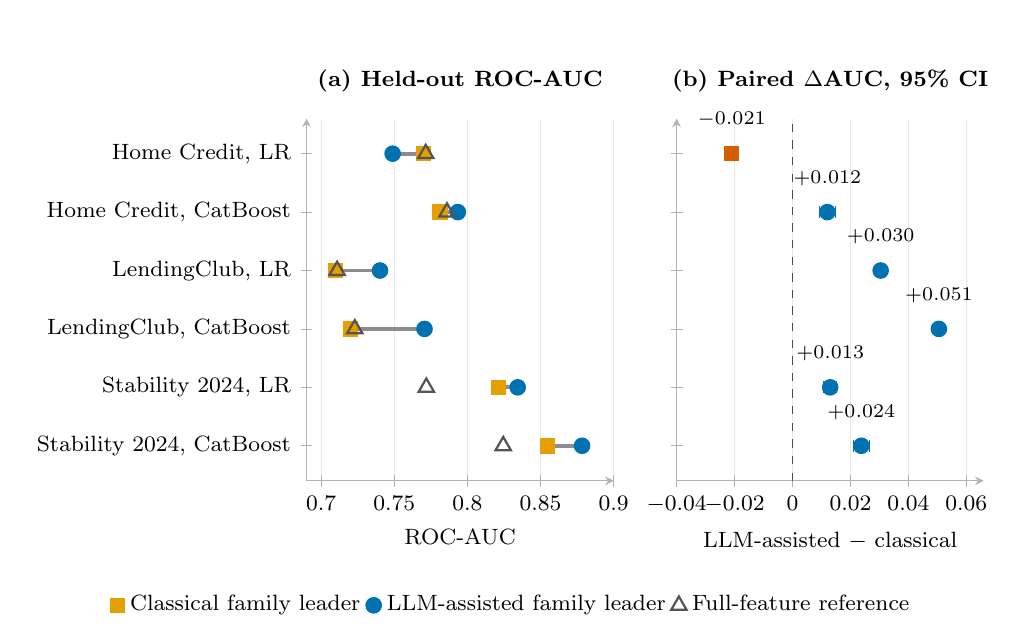
\begin{tikzpicture}
\begin{groupplot}[
    paper,
    group style={group size=2 by 1, horizontal sep=8mm, y descriptions at=edge left},
    scale only axis, width=3.9cm, height=4.6cm,
    ymin=0.4, ymax=6.6, ytick={1,2,3,4,5,6},
    yticklabels={{Stability 2024, CatBoost},{Stability 2024, LR},{LendingClub, CatBoost},{LendingClub, LR},{Home Credit, CatBoost},{Home Credit, LR}},
    xmajorgrids, axis lines=left, clip=false,
    xticklabel style={/pgf/number format/fixed, /pgf/number format/precision=2},
]
\nextgroupplot[title={(a) Held-out ROC-AUC}, xlabel={ROC-AUC}, xmin=0.69, xmax=0.90, xtick={0.70,0.75,0.80,0.85,0.90},
    legend to name=primlegend, legend columns=3]
\addplot[cGrey, line width=1.4pt, forget plot] coordinates {(0.854644,1) (0.878400,1)};
\addplot[cGrey, line width=1.4pt, forget plot] coordinates {(0.821394,2) (0.834400,2)};
\addplot[cGrey, line width=1.4pt, forget plot] coordinates {(0.720147,3) (0.770664,3)};
\addplot[cGrey, line width=1.4pt, forget plot] coordinates {(0.709803,4) (0.740234,4)};
\addplot[cGrey, line width=1.4pt, forget plot] coordinates {(0.781426,5) (0.793450,5)};
\addplot[cGrey, line width=1.4pt, forget plot] coordinates {(0.769890,6) (0.748857,6)};
\addplot[only marks, mark=square*, mark size=2.6pt, cOrange]
    coordinates {(0.854644,1) (0.821394,2) (0.720147,3) (0.709803,4) (0.781426,5) (0.769890,6)};
\addlegendentry{Classical family leader}
\addplot[only marks, mark=*, mark size=2.8pt, cBlue]
    coordinates {(0.878400,1) (0.834400,2) (0.770664,3) (0.740234,4) (0.793450,5) (0.748857,6)};
\addlegendentry{LLM-assisted family leader}
\addplot[only marks, mark=triangle, mark size=3.2pt, thick, cGrey!60!black]
    coordinates {(0.82449,1) (0.77191,2) (0.722973,3) (0.710887,4) (0.786032,5) (0.771496,6)};
\addlegendentry{Full-feature reference}
\nextgroupplot[title={(b) Paired $\Delta$AUC, 95\% CI}, xlabel={LLM-assisted $-$ classical}, xmin=-0.04, xmax=0.066, xtick={-0.04,-0.02,0,0.02,0.04,0.06}]
\draw[gray!60!black, dashed] (axis cs:0,0.4) -- (axis cs:0,6.6);
\addplot[only marks, mark=*, mark size=2.8pt, cBlue,
    error bars/.cd, x dir=both, x explicit,
    error bar style={line width=1pt, cBlue},
    error mark options={rotate=90, mark size=2.2pt, cBlue}]
    coordinates {
        (0.023756,1) -= (0.002795,0) += (0.002855,0)
        (0.013006,2) -= (0.002365,0) += (0.002265,0)
        (0.050517,3) -= (0.000805,0) += (0.000798,0)
        (0.030431,4) -= (0.001072,0) += (0.001083,0)
        (0.012024,5) -= (0.002711,0) += (0.002817,0)
    };
\addplot[only marks, mark=square*, mark size=2.6pt, cRed,
    error bars/.cd, x dir=both, x explicit,
    error bar style={line width=1pt, cRed},
    error mark options={rotate=90, mark size=2.2pt, cRed}]
    coordinates { (-0.021033,6) -= (0.001178,0) += (0.001253,0) };
\node[font=\scriptsize, above=6pt] at (axis cs:0.023756,1) {$+0.024$};
\node[font=\scriptsize, above=6pt] at (axis cs:0.013006,2) {$+0.013$};
\node[font=\scriptsize, above=6pt] at (axis cs:0.050517,3) {$+0.051$};
\node[font=\scriptsize, above=6pt] at (axis cs:0.030431,4) {$+0.030$};
\node[font=\scriptsize, above=6pt] at (axis cs:0.012024,5) {$+0.012$};
\node[font=\scriptsize, above=6pt] at (axis cs:-0.021033,6) {$-0.021$};
\end{groupplot}
\node[anchor=north, yshift=-2mm] at (current bounding box.south) {\pgfplotslegendfromname{primlegend}};
\end{tikzpicture}
\caption{Primary held-out (HO) comparison. (a) ROC-AUC of the classical family leader, the LLM-assisted family leader (the selector with the highest observed HO AUC within its family) and the untuned full-feature reference in each dataset--backbone case; the grey bar joins the two selectors being compared. (b) Paired difference, LLM-assisted minus classical, with its 95\% confidence interval; positive values favour LLM-assisted selection and the red square marks the one case in which the classical selector is higher. The intervals are paired bootstrap intervals, not adjusted for the selection of the compared methods on the same HO results; the comparison is descriptive, and Table~\ref{tab:confirmatory} gives the development-rule comparison with leaders chosen on development data.}
\label{fig:primary}
\end{figure*}

\subsection{Secondary Metrics}
\label{subsec:secondary_results}

Table~\ref{tab:secondary} reports the best held-out (HO) value of each secondary metric in each dataset with the pipeline attaining it; the leaders are not always the same pipeline, so the values describe the frontier reached by the selector family rather than one model. The best KS is attained by an LLM-assisted CatBoost pipeline in all three datasets, and the best top-decile concentration by pure LLM in all three, with CatBoost on Home Credit and Stability 2024 and logistic regression on LendingClub, at Lift@10 of 3.63, 2.75 and 4.67; the best Brier score is attained by an LLM-assisted CatBoost pipeline in each dataset. The best Brier score is the lowest among the evaluated selectors and not evidence of good absolute calibration: both backbones use balanced class weights and no recalibration, so their outputs are not population event probabilities, and Brier measures overall squared probability error rather than calibration alone. Feature drift is reported for the twelve headline pipelines of Table~\ref{tab:primary_results}, as the mean, median and maximum DEV-versus-HO PSI of the features each leader's frozen full-DEV refit selected. All values are small: mean selected-feature PSI runs from 0.0024 to 0.0189 across the twelve subsets, and no feature of any subset exceeds a PSI of 0.115. The LLM-assisted leader has the lower mean drift than the classical leader of the same case in five of the six cases and the lower median in all six: means of 0.0053 against 0.0085 and 0.0045 against 0.0097 on Home Credit, 0.0125 against 0.0129 and 0.0104 against 0.0125 on LendingClub, and 0.0024 against 0.0189 on Stability 2024 CatBoost; the exception is Stability 2024 logistic regression, where pure LLM's mean of 0.0174 exceeds RFE CatBoost's 0.0092 while its median, 0.0023 against 0.0042, is still the lower. The median feature PSI of the pure LLM CatBoost subset on Home Credit is 0.0035, and on Stability 2024 CatBoost 0.0001, meaning that for the typical selected variable almost no distribution difference was detected under the implemented states, binning and precision. The largest single-feature drift in a headline subset is 0.114, a tax-registry row count in the CatBoost SHAP subset on Stability 2024, followed by 0.086 for a count of instalments without delinquency in the pure LLM subset of the same case and 0.058 for an instalment-timing variance in the RFE CatBoost subset on Home Credit; on Home Credit, where the held-out population is shifted in prior-application recency, the most drifted selected feature of every leader is a bureau, instalment or credit-card field rather than a previous-application recency field. Lower drift within the selected inputs is reported as a property of the subsets and not as an explanation of the AUC ordering (Section~\ref{subsec:performance_vs_stability}).

\begin{table*}[htbp]
\centering
\footnotesize
\begin{threeparttable}
\caption{Best held-out (HO) secondary metric in each dataset, with the selector and backbone attaining it. KS is the maximum separation over HO thresholds; Brier is lower-is-better; Capture@10 is the share of events in the highest-scored decile, with Lift@10 in parentheses.}
\label{tab:secondary}
\begin{tabular}{@{}lL{29mm}L{29mm}L{35mm}@{}}
\toprule
Dataset & KS & Brier score & Capture@10 (Lift@10) \\
\midrule
Home Credit & 0.4264\newline Pure LLM, CatBoost & 0.1234\newline Pure LLM, CatBoost & 0.3630 (3.63)\newline Pure LLM, CatBoost \\
\addlinespace
LendingClub v2 & 0.3898\newline LLM then mRMR, CatBoost & 0.1824\newline LLM then mRMR, CatBoost & 0.2751 (2.75)\newline Pure LLM, LR \\
\addlinespace
Stability 2024 & 0.5559\newline Pure LLM, CatBoost & 0.1592\newline Pure LLM, CatBoost & 0.4671 (4.67)\newline Pure LLM, CatBoost \\
\bottomrule
\end{tabular}
\end{threeparttable}
\end{table*}

\subsection{Feature-Selection Stability}
\label{subsec:stability_results}

Table~\ref{tab:stability} and Figure~\ref{fig:stability} report fold-to-fold reproducibility (RQ2). Among independently refitted classical selectors, Boruta RF on LendingClub logistic regression is the most reproducible selector in the study (Nogueira 0.9588, Jaccard 0.9273); IV/WOE leads four of the six cases and mRMR leads LendingClub CatBoost. Stability is lowest on Stability 2024, whose candidate set of 1,068 features is by far the largest (Nogueira about 0.78, Jaccard about 0.66). The pure LLM lists were requested separately per fold partition rather than refitted, and Table~\ref{tab:stability} reports their fold agreement over the candidate set on Home Credit and LendingClub, where five fold lists exist per case; the cached rankings all differ, the six of 100 names on Home Credit and all 24 on LendingClub. Their agreement is among the lowest in the table, with LLM then Boruta: Nogueira 0.41 to 0.63 and mean pairwise Jaccard 0.31 to 0.48, the top-20 lists sharing pairwise Jaccard between 0.25 and 0.67 on Home Credit and between 0.25 and 0.60 on LendingClub, and the top-40 lists between 0.23 and 0.51 and between 0.40 and 0.54. The fold-pair spreads of the pure LLM lists, 0.14 to 0.42 wide, are comparable in width to those of the classical leaders, 0.18 to 0.42, so the lists differ at a lower level of agreement rather than more erratically. The ordering holds pair by pair: on Home Credit and LendingClub the least similar fold pair of the classical leader is at least as similar as the most similar pair of the pure LLM list of the same case (0.667 against 0.667, a tie, 0.667 against 0.509, 0.818 against 0.600 and 0.702 against 0.538), so the difference between the two families in Table~\ref{tab:stability} does not rest on a single fold split. Of the 20 features in a Home Credit logistic regression list, 6 appear in all five folds and the five lists together span 42 names; at $\Kfeat=40$ the counts are 8 and 98; on LendingClub they are 4 and 39 at $\Kfeat=20$ and 14 and 71 at $\Kfeat=40$. On Stability 2024 one ranking served every fold, so its fold agreement is 1 by construction and is not reported; in its place the sampling of the model at a fixed prompt was isolated directly by repeating the full-DEV call ten times with the same prompt, snapshot, temperature 0 and the same 1,068 candidate records. All ten responses passed the same strict validation as the cached one, and the ten rankings of 100 names are all distinct. Over that candidate set the ten lists reach Nogueira 0.8052 with mean pairwise Jaccard 0.6908 at $\Kfeat=20$ and 0.7766 with 0.6506 at $\Kfeat=40$; 11 of the 20 names and 22 of the 40 appear in all ten responses, and the ten lists together span 30 and 69 distinct names. Response sampling alone therefore leaves the semantic ranking on this dataset level with the classical leader of the same case over the same universe (0.7860 and 0.7793); its mean pairwise Jaccard at $\Kfeat=20$, 0.6908, exceeds that leader's fold mean of 0.6666 and lies inside the leader's fold-pair range of 0.481 to 0.905. The pure LLM rows for Home Credit and LendingClub measure the same quantity, the candidate list being fixed there too (Section~\ref{subsec:llm_fs}), and are much lower; because the chance correction depends on $d$ (Section~\ref{subsec:fs_stability_background}) the three are not on a common scale and the comparison between datasets is not made here. Carrying each response through the frozen downstream pipeline gives held-out AUC from 0.8300 to 0.8395 at $\Kfeat=20$ (median 0.8350, s.d.\ 0.0030) and from 0.8740 to 0.8832 at $\Kfeat=40$ (median 0.8764, s.d.\ 0.0030); the cached values of Table~\ref{tab:primary_results}, 0.8344 and 0.8784, lie above four and above seven of the ten repeats, inside the body of the distribution rather than at its top. The margin over the classical leader stays positive in all twenty refits, $+0.0086$ to $+0.0181$ against RFE CatBoost (0.8214) and $+0.0194$ to $+0.0286$ against CatBoost SHAP (0.8546), so no repeat reverses the direction of the comparison, and only two of the ten logistic-regression repeats fall below the materiality bar of 0.010 (Section~\ref{subsec:inference}), by 0.0014 and 0.0003, while every CatBoost repeat clears it. Both spreads, 0.0095 at $\Kfeat=20$ and 0.0092 at $\Kfeat=40$, are themselves inside that bar, so on this dataset the choice of cached response is immaterial at both budgets by the study's own standard. These twenty refits vary the response only and are not a confidence interval; they are reported beside, not inside, the paired bootstrap intervals of Section~\ref{subsec:inference}. The hybrids' final subsets depend on both the per-fold semantic ranking and the fitted statistical stage: stable core plus LLM fill reaches Nogueira 0.69 to 0.76 and Jaccard 0.57 to 0.63 in the six cases, below the classical leader of the same case by 0.03 to 0.25 in Nogueira and above pure LLM by 0.08 to 0.28. Its fold pairs reach the classical range: in all six cases its most similar pair is at or above the least similar pair of the classical leader (0.818 against 0.818 on LendingClub logistic regression, a tie, and 0.905 against 0.481 on Stability 2024 logistic regression), so the construction recovers classical-level agreement on part of the fold pairs, whereas LLM then Boruta lies between 0.42 and 0.63 in all six cases. On Home Credit and LendingClub it is level with the pure LLM lists it refits on, within 0.04 in three of the four cases and 0.11 below on Home Credit logistic regression; on Stability 2024, where one semantic ranking served every fold, its 0.49 (logistic regression) and 0.55 (CatBoost) are produced by the Boruta refit alone. Refitting Boruta on the semantic candidates therefore does not recover the reproducibility that the ranking loses, and with the ranking held fixed it leaves the subsets 0.16 to 0.27 below the stable core construction of the same case (0.7554 and 0.7091) and 0.23 to 0.30 below the classical leader (0.7860 and 0.7793); the stable core construction recovers part of what the ranking loses, and the classical leaders exceed pure LLM by 0.28 to 0.43 in Nogueira. The six CLIP-ranked cells on Stability 2024 reach Nogueira 0.683 to 0.753 and Jaccard 0.657 to 0.723, the Home Credit source with logistic regression being the most reproducible cell on both measures. These values are computed over candidate pools of 60 or 100 features, not over the 1,068-feature candidate set used for the classical selectors, so the two groups are not on the same scale and the table does not rank them against each other. In Figure~\ref{fig:stability} the CLIP cells lie close to the identity line while the classical leaders and the pure LLM lists fall below it, because the Nogueira universe of a CLIP cell is its small candidate pool, so the chance correction is large and $\hat\Phi$ is close to the uncorrected Jaccard, whereas over the candidate set the correction is small and $\hat\Phi$ exceeds Jaccard. For the same fold subsets a smaller universe gives a lower $\hat\Phi$.

\begin{table*}[htbp]
\centering
\footnotesize
\begin{threeparttable}
\caption{Fold-to-fold reproducibility across the five development folds: the most reproducible independently refitted classical selector in each case (Nogueira stability as primary ordering, mean pairwise Jaccard as tie-breaker), the six CLIP-ranked cells on Stability 2024, the two LLM hybrids whose final subset is fixed by a refitted statistical stage, and the pure LLM lists cached per fold on Home Credit and LendingClub. Jaccard is the mean pairwise Jaccard over the ten fold pairs; Min and Max are its minimum and maximum over the same pairs. $d$ is the Nogueira universe; $P$ is the pool passed to the RF/correlation filter.}
\label{tab:stability}
\setlength{\tabcolsep}{4pt}
\begin{tabular}{@{}lllcrrrr@{}}
\toprule
Case & Model & Selector & $\Kfeat$ & Nogueira & Jaccard & Min & Max\tnote{b} \\
\midrule
\multicolumn{8}{@{}l}{\emph{Refitted classical selectors ($d$ = the candidate set: 373, 675 and 1,068)}} \\
Home Credit & LR & IV/WOE & 20 & 0.8838 & 0.8053 & 0.667 & 0.905 \\
Home Credit & CatBoost & IV/WOE & 40 & 0.8403 & 0.7538 & 0.667 & 0.905 \\
LendingClub v2 & LR & Boruta RF & 20 & 0.9588 & 0.9273 & 0.818 & 1.000 \\
LendingClub v2 & CatBoost & mRMR & 40 & 0.9070 & 0.8462 & 0.702 & 1.000 \\
Stability 2024 & LR & IV/WOE & 20 & 0.7860 & 0.6666 & 0.481 & 0.905 \\
Stability 2024 & CatBoost & IV/WOE & 40 & 0.7793 & 0.6582 & 0.509 & 0.905 \\
\addlinespace
\multicolumn{8}{@{}l}{\emph{CLIP-ranked selection on Stability 2024}} \\
\multicolumn{8}{@{}l}{\emph{($d=P$; $P=60$ for LR, $P=100$ for CatBoost)}} \\
Stability $\rightarrow$ Stability & LR & CLIP-ranked & 20 & 0.7225 & 0.6973 & -- & -- \\
Stability $\rightarrow$ Stability & CatBoost & CLIP-ranked & 40 & 0.6833 & 0.6889 & -- & -- \\
Home Credit $\rightarrow$ Stability & LR & CLIP-ranked & 20 & 0.7525 & 0.7225 & -- & -- \\
Home Credit $\rightarrow$ Stability & CatBoost & CLIP-ranked & 40 & 0.7125 & 0.7101 & -- & -- \\
LendingClub $\rightarrow$ Stability & LR & CLIP-ranked & 20 & 0.6850 & 0.6567 & -- & -- \\
LendingClub $\rightarrow$ Stability & CatBoost & CLIP-ranked & 40 & 0.7208 & 0.7175 & -- & -- \\
\addlinespace
\multicolumn{8}{@{}l}{\emph{LLM hybrids with a refitted statistical stage}} \\
\multicolumn{8}{@{}l}{\emph{($d$ = the candidate set: 373, 675 and 1,068)}} \\
Home Credit & LR & Stable core + LLM fill & 20 & 0.7411 & 0.6110 & 0.481 & 0.818 \\
Home Credit & CatBoost & Stable core + LLM fill & 40 & 0.6920 & 0.5725 & 0.455 & 0.739 \\
LendingClub v2 & LR & Stable core + LLM fill & 20 & 0.7115 & 0.5783 & 0.379 & 0.818 \\
LendingClub v2 & CatBoost & Stable core + LLM fill & 40 & 0.7130 & 0.5842 & 0.404 & 0.778 \\
Stability 2024 & LR & Stable core + LLM fill & 20 & 0.7554 & 0.6259 & 0.429 & 0.905 \\
Stability 2024 & CatBoost & Stable core + LLM fill & 40 & 0.7091 & 0.5727 & 0.379 & 0.778 \\
Home Credit & LR & LLM then Boruta & 20 & 0.4294 & 0.3031 & 0.212 & 0.429 \\
Home Credit & CatBoost & LLM then Boruta & 40 & 0.4204 & 0.3247 & 0.194 & 0.509 \\
LendingClub v2 & LR & LLM then Boruta & 20 & 0.5414 & 0.4103 & 0.143 & 0.739 \\
LendingClub v2 & CatBoost & LLM then Boruta & 40 & 0.6333 & 0.4920 & 0.379 & 0.702 \\
Stability 2024 & LR & LLM then Boruta & 20 & 0.4876 & 0.3682 & -- & -- \\
Stability 2024 & CatBoost & LLM then Boruta & 40 & 0.5528 & 0.4193 & -- & -- \\
\addlinespace
\multicolumn{8}{@{}l}{\emph{Pure LLM, cached per-fold lists ($d$ = the candidate set: 373 and 675)}\tnote{a}} \\
Home Credit & LR & Pure LLM & 20 & 0.5403 & 0.4076 & 0.250 & 0.667 \\
Home Credit & CatBoost & Pure LLM & 40 & 0.4092 & 0.3149 & 0.231 & 0.509 \\
LendingClub v2 & LR & Pure LLM & 20 & 0.5517 & 0.4011 & 0.250 & 0.600 \\
LendingClub v2 & CatBoost & Pure LLM & 40 & 0.6280 & 0.4828 & 0.404 & 0.538 \\
\bottomrule
\end{tabular}
\begin{tablenotes}\footnotesize
\item[a] Lists requested separately for each fold partition, not refitted; because the candidate set is the same in every call, a fold-to-fold difference reflects the sampling of the language model at a fixed prompt. The Nogueira universe is the same screened candidate set as for every other row of the dataset, 373 features on Home Credit and 675 on LendingClub, so the pure LLM rows are on a common scale with the classical and hybrid rows. Stability 2024 is absent because one ranking served every fold, so its fold agreement is 1 by construction.
\item[b] Minimum and maximum pairwise Jaccard over the ten fold pairs, from the same fold lists as the mean; not reported for the CLIP cells and for the two Stability 2024 LLM then Boruta rows.
\end{tablenotes}
\end{threeparttable}
\end{table*}

\begin{figure*}[htbp]
\centering
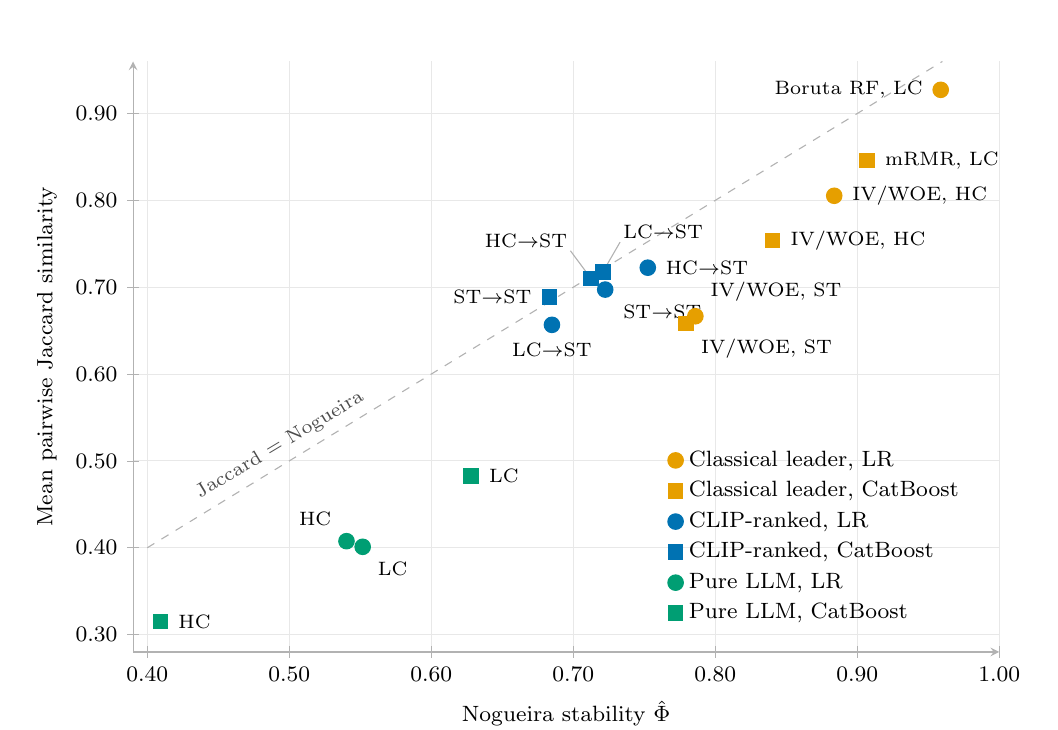
\begin{tikzpicture}
\begin{axis}[
    paper,
    scale only axis, width=11cm, height=7.5cm,
    axis lines=left, clip=false,
    xlabel={Nogueira stability $\hat\Phi$}, ylabel={Mean pairwise Jaccard similarity},
    xmin=0.39, xmax=1.00, ymin=0.28, ymax=0.96,
    xtick={0.40,0.50,0.60,0.70,0.80,0.90,1.00},
    ytick={0.30,0.40,0.50,0.60,0.70,0.80,0.90},
    xticklabel style={/pgf/number format/fixed, /pgf/number format/precision=2, /pgf/number format/zerofill},
    yticklabel style={/pgf/number format/fixed, /pgf/number format/precision=2, /pgf/number format/zerofill},
    xmajorgrids, ymajorgrids,
    legend pos=south east, legend cell align=left,
]
\addplot[domain=0.40:0.96, samples=2, dashed, gray!60, forget plot] {x};
\node[font=\scriptsize, gray!60!black, rotate=31, anchor=south] at (axis cs:0.50,0.50) {Jaccard $=$ Nogueira};
\addplot[only marks, mark=*, mark size=2.8pt, cOrange]
    coordinates {(0.8838,0.8053) (0.9588,0.9273) (0.7860,0.6666)};
\addlegendentry{Classical leader, LR}
\addplot[only marks, mark=square*, mark size=2.6pt, cOrange]
    coordinates {(0.8403,0.7538) (0.9070,0.8462) (0.7793,0.6582)};
\addlegendentry{Classical leader, CatBoost}
\addplot[only marks, mark=*, mark size=2.8pt, cBlue]
    coordinates {(0.7225,0.6973) (0.7525,0.7225) (0.6850,0.6567)};
\addlegendentry{CLIP-ranked, LR}
\addplot[only marks, mark=square*, mark size=2.6pt, cBlue]
    coordinates {(0.6833,0.6889) (0.7125,0.7101) (0.7208,0.7175)};
\addlegendentry{CLIP-ranked, CatBoost}
\addplot[only marks, mark=*, mark size=2.8pt, cGreen]
    coordinates {(0.5403,0.4076) (0.5517,0.4011)};
\addlegendentry{Pure LLM, LR}
\addplot[only marks, mark=square*, mark size=2.6pt, cGreen]
    coordinates {(0.4092,0.3149) (0.6280,0.4828)};
\addlegendentry{Pure LLM, CatBoost}
\node[font=\scriptsize, anchor=south east, xshift=-2pt, yshift=2pt] at (axis cs:0.5403,0.4076) {HC};
\node[font=\scriptsize, anchor=north west, xshift=2pt, yshift=-2pt] at (axis cs:0.5517,0.4011) {LC};
\node[font=\scriptsize, anchor=west, xshift=3pt] at (axis cs:0.4092,0.3149) {HC};
\node[font=\scriptsize, anchor=west, xshift=3pt] at (axis cs:0.6280,0.4828) {LC};
\node[font=\scriptsize, anchor=west, xshift=3pt] at (axis cs:0.8838,0.8053) {IV/WOE, HC};
\node[font=\scriptsize, anchor=west, xshift=3pt] at (axis cs:0.8403,0.7538) {IV/WOE, HC};
\node[font=\scriptsize, anchor=east, xshift=-3pt] at (axis cs:0.9588,0.9273) {Boruta RF, LC};
\node[font=\scriptsize, anchor=west, xshift=3pt] at (axis cs:0.9070,0.8462) {mRMR, LC};
\node[font=\scriptsize, anchor=south west, xshift=2pt, yshift=2pt] at (axis cs:0.7860,0.6666) {IV/WOE, ST};
\node[font=\scriptsize, anchor=north west, xshift=2pt, yshift=-2pt] at (axis cs:0.7793,0.6582) {IV/WOE, ST};
\node[font=\scriptsize, anchor=north west, xshift=3pt, yshift=-2pt] at (axis cs:0.7225,0.6973) {ST$\rightarrow$ST};
\node[font=\scriptsize, anchor=east, xshift=-3pt] at (axis cs:0.6833,0.6889) {ST$\rightarrow$ST};
\node[font=\scriptsize, anchor=west, xshift=3pt] at (axis cs:0.7525,0.7225) {HC$\rightarrow$ST};
\draw[gray!60, thin] (axis cs:0.7125,0.7101) -- (axis cs:0.6980,0.7420);
\node[font=\scriptsize, anchor=south east, inner sep=1pt] at (axis cs:0.6980,0.7420) {HC$\rightarrow$ST};
\node[font=\scriptsize, anchor=north, yshift=-3pt] at (axis cs:0.6850,0.6567) {LC$\rightarrow$ST};
\draw[gray!60, thin] (axis cs:0.7208,0.7175) -- (axis cs:0.7330,0.7520);
\node[font=\scriptsize, anchor=south west, inner sep=1pt] at (axis cs:0.7330,0.7520) {LC$\rightarrow$ST};
\end{axis}
\end{tikzpicture}
\caption{Reproducibility landscape of fold-level selections. Orange: most reproducible refitted classical selector in each dataset--backbone case; blue: CLIP-ranked cells on Stability 2024, labelled source$\rightarrow$target; green: pure LLM lists cached per fold on Home Credit and LendingClub. Circles are logistic regression ($\Kfeat=20$), squares CatBoost ($\Kfeat=40$). HC = Home Credit, LC = LendingClub v2, ST = Stability 2024. Higher is more reproducible on both axes; the dashed line marks equality of the two statistics. The Nogueira universe is the screened candidate set for the classical leaders and the pure LLM lists and the 60- or 100-feature candidate pool for the CLIP cells, so the CLIP cells are not on a common scale with the other two groups.}
\label{fig:stability}
\end{figure*}

\subsection{Name Obfuscation on Home Credit}
\label{subsec:obfuscation_results}

Table~\ref{tab:obfuscation} reports the two obfuscated arms of Section~\ref{subsec:llm_fs} against the named pure LLM pipelines of Table~\ref{tab:llm_pipelines}, on the same HO observations. With the names replaced by identifiers and the definitions kept (arm A), the held-out AUC is unchanged: 0.7424 against 0.7436 with logistic regression and 0.7977 against 0.7935 with CatBoost, differences of $-0.0012$ and $+0.0042$, both inside the materiality bar of 0.010 (Section~\ref{subsec:inference}). With the names kept and the definitions removed (arm B), the AUC falls under both backbones, to 0.7146 and 0.7625, by $-0.0290$ and $-0.0310$, three times the bar. The lists themselves change more than the AUC does. In every named Home Credit call the three external scores occupy ranks 1, 2 and 3, an order that nothing in their metadata can produce, since the three records are identical apart from the digit; in arm A they fall to ranks 10 to 18 in the five fold calls and to ranks 12, 57 and 13 in the full-DEV call, while in arm B they sit at ranks 6, 7 and 8 in all six calls. On the full-DEV partition arm A shares 11 of the 20 names of the named logistic-regression subset and 17 of the 40 names of the named CatBoost subset (\ref{app:subsets}); arm B shares 14 and 24. Across the five fold calls the arm A lists agree with one another more than the named lists do, pairwise Jaccard 0.43 to 1.00 at $\Kfeat=20$ (mean 0.60) against 0.25 to 0.67 (mean 0.41) for the named lists (Section~\ref{subsec:stability_results}), and the arm B lists more still, 0.67 to 1.00 (mean 0.78). The reading is the first of the three fixed before the run: the AUC holds without the names while the lists partly overlap, so the value of the ranking rests on the definitions, and the familiar names shaped the top of the named lists without carrying their predictive value. Two limits apply. Obfuscating a name leaves a definition that may itself be recognisable, so the ablation weakens the name channel rather than removing it; and the comparison is descriptive, the differences of arm A being smaller than the fold-to-fold spread of a single arm, and covers Home Credit only, the dataset on which the exposure is largest (Section~\ref{subsec:limitations}).

\begin{table*}[htbp]
\centering
\footnotesize
\begin{threeparttable}
\caption{Name-obfuscation ablation on Home Credit. Held-out AUC of the pure LLM pipeline when the six ranking calls are repeated with the feature names replaced by seeded identifiers (arm A, definitions kept) or with the definitions removed (arm B, names kept), against the named cached rankings; same HO observations, same fixed backbones. Fold range is the span of the five fold-model AUCs. Overlap is the number of names the arm's full-DEV subset shares with the named full-DEV subset of the same budget (\ref{app:subsets}). Ranks of the three external scores are given for the full-DEV call.}
\label{tab:obfuscation}
\begin{tabular}{@{}llcrrrlr@{}}
\toprule
Arm & Model & $\Kfeat$ & HO AUC & Named & $\Delta$ & Fold range & Overlap \\
\midrule
A, names removed & LR & 20 & 0.7424 & 0.7436 & $-0.0012$ & 0.721--0.741 & 11/20 \\
A, names removed & CatBoost & 40 & 0.7977 & 0.7935 & $+0.0042$ & 0.751--0.785 & 17/40 \\
B, definitions removed & LR & 20 & 0.7146 & 0.7436 & $-0.0290$ & 0.706--0.735 & 14/20 \\
B, definitions removed & CatBoost & 40 & 0.7625 & 0.7935 & $-0.0310$ & 0.731--0.753 & 24/40 \\
\bottomrule
\end{tabular}
\begin{tablenotes}\footnotesize
\item Ranks of \texttt{EXT\_SOURCE\_1/2/3} in the full-DEV call: named 1, 2, 3; arm A 12, 57, 13; arm B 6, 7, 8.
\end{tablenotes}
\end{threeparttable}
\end{table*}

\subsection{Cost and Runtime of the Pre-Screening Stage}
\label{subsec:cost_runtime}

On Home Credit and LendingClub, 72 logical screening requests were served by 30 provider ranking calls, 6 on Home Credit and 24 on LendingClub, the remainder being cache hits. The 30 calls consumed 806,757 input and 56,495 output tokens, for a direct API cost between USD~0.171 and USD~0.413 at the GPT-4.1 mini list prices of USD~0.40 per million input tokens, 0.10 per million cached input tokens and 1.60 per million output tokens; the bounds correspond to all input charged at the cached rate and at the uncached rate. The Stability 2024 ranking call is not included, because its token usage was not recorded. Wall-clock times were not measured under matched conditions, with the one exception noted at the end of this section, and support no scalability claim. On Home Credit logistic regression the pure LLM pipeline took 0.8 minutes against 12.1 minutes for full-pool mRMR (RF/correlation implementation) and 24.6 minutes for stable core plus LLM fill. On LendingClub CatBoost pure LLM was slower than mRMR: domain rules took 49.7 minutes, mRMR 65.3, LLM then mRMR 72.8, pure LLM 73.8, PCA 88.0, LLM then Boruta 110.5, Boruta 172.6 and stable core plus LLM fill 256.0 minutes, of which 176.6 minutes were feature selection; measured against the 49.7 minutes of the essentially selection-free domain-rules pipeline, it is the selection stage rather than model fitting that separates the pipelines, and the semantic call is negligible beside both. The saved runs of the final protocol were executed on the CPU of one machine with 16 logical (10 physical) cores and 39.6~GiB of RAM, with four estimator threads and no accelerator; peak process memory was 7.4 to 10.7~GB for the Home Credit selectors and full-feature references, 19.1 to 29.0~GB for their LendingClub counterparts and 27.0 to 29.0~GB for their Stability 2024 counterparts. Runtimes were measured under unequal caching and execution conditions and are quoted above for Home Credit and LendingClub only. One downstream saving from a reduced candidate pool was measured under matched conditions: on Stability 2024 fold 1, on the same machine, the mRMR stage took 522 seconds over the 1,959-feature universe and 21 seconds over a 100-feature pool, a factor of 25 for a pool twenty times smaller.



% ============================================================
% 7. DISCUSSION
% ============================================================

\section{Discussion}
\label{sec:discussion}

\subsection{Main Findings}
\label{subsec:main_findings}

RQ1 asked whether an LLM pre-screened subset can match or exceed classically selected subsets on held-out data under a fixed budget. The answer is conditional: in five of six dataset--backbone cases the LLM-assisted family leader exceeds the classical family leader, whether the leaders are chosen on the HO results, in which case the comparison is descriptive, or on the development folds, in which case all six differences are Holm-significant (Section~\ref{subsec:inference}, Table~\ref{tab:confirmatory}); on Home Credit logistic regression the classical leader is higher under both rules, mutual-information mRMR by 0.021 and IV then Boruta by 0.010. The pattern does not depend on comparing family leaders: by mean HO AUC over the selectors that are not declared floors, the LLM-assisted family is ahead in the same five cases and behind on Home Credit logistic regression (Section~\ref{subsec:primary_results}). The leading LLM-assisted method is pure LLM in four cases, LLM then mRMR in one (LendingClub v2 CatBoost) and stable core plus LLM fill in the Home Credit logistic-regression case that the classical selector wins. Within these comparisons the semantic ranking therefore most often had the higher HO AUC when used directly; statistical refinement of the semantic pool led in one case, and on Home Credit CatBoost the refined pipeline (0.7758, LLM then mRMR, Table~\ref{tab:llm_pipelines}) had a lower held-out AUC than pure LLM (0.7935). Direct use of the semantic ranking and statistical refinement are alternatives whose observed value differed by dataset and backbone. The results establish neither arrangement as generally preferable, nor LLM pre-screening as a replacement for statistical selection. The choice between them for a deployed pipeline is a development-stage decision, to be made on development data rather than on the holdout used to report final performance, which is how the leaders of Table~\ref{tab:primary_results} were identified and why Table~\ref{tab:confirmatory} repeats the comparison with leaders chosen on development data. The full-feature reference was not tuned for the wide problem, so the study makes no claim about compact subsets against the full feature set. On reproducibility (RQ2), refitted classical selectors reach Nogueira stability between 0.78 and 0.96, with information value and Boruta the most reproducible, whereas the pure LLM lists of the discrimination-leading pipelines differ from fold to fold, Nogueira 0.41 to 0.63 over the same candidate set (Section~\ref{subsec:stability_results}); the best-discriminating selector in this study is, with LLM then Boruta, the least reproducible one in Table~\ref{tab:stability}, and its reported AUC is that of the particular cached responses. Ten repeated calls on the Stability 2024 partition bound how much that last point costs there: the ranking varies (Nogueira 0.8052 and 0.7766) but the held-out AUC moves by 0.0095 and 0.0092, inside the materiality bar, and the direction of the comparison holds in every repeat (Section~\ref{subsec:stability_results}).

The obfuscation ablation (Section~\ref{subsec:obfuscation_results}) addresses the reading of the contribution that the study could not otherwise exclude, recognition of familiar feature names rather than semantic pre-screening. On Home Credit, the dataset whose variable book is most widely documented, replacing every name by a seeded identifier leaves the held-out AUC of the pure LLM pipeline within 0.005 of the named result under both backbones, while removing the definitions and keeping the names costs about 0.03. The ranking's value therefore rests on what the definitions say, not on which names appear. The names did leave a trace: in every named call the three external scores are ranked 1, 2, 3, an order the identical metadata of the three cannot produce, and it disappears when the names do. That ordering is reported here rather than left for a referee to find because it is the clearest evidence of recall in the study, and the ablation shows that it did not carry the result. The test covers one dataset and weakens rather than removes the name channel, since a definition can itself be recognisable; its scope is stated in Section~\ref{subsec:limitations}.

\subsection{Supplementary Experiments: Contrastive Transfer and Rank Voting}
\label{subsec:supplementary_discussion}

The contrastive representation (\ref{app:clip}) addressed whether a feature representation learned on one portfolio transfers to another. Representations trained on three portfolios rank the same Stability 2024 predictors very differently, the Home Credit and LendingClub sources sharing one of their top-100 features, so the experiment shows source dependence rather than transfer; every transferred ranking still supports a model whose HO AUC exceeds its development estimate, on the earlier Stability cohort. The contrastive ranking followed by the RF/correlation filter reaches Nogueira stability of 0.68 to 0.75 over its candidate pools of 60 or 100 features, a universe not comparable with the classical one. In the earlier Home Credit experiments, under the protocol of that version (Table~\ref{tab:stages}), inserting the representation into an LLM-screened pipeline raised fold-to-fold Jaccard similarity by 0.32 to 0.50 while HO AUC changed by less than 0.002. The isolated contribution of the representation was not established, and the branch is descriptive throughout.

The rank-voting experiment (\ref{app:voting}) asked whether parallel combination of rankings recovers information that sequential screening discards. Parallel voting does not improve on sequential screening on Home Credit: it exceeds the sequential pipeline in two of eight point estimates, by at most $+0.0014$, lies below it in the other six, and exceeds mRMR on the whole candidate set in one of eight (CatBoost, $P=300$, $+0.0065$). The voting variants differ from the sequential pipeline in pool size and in the rankings combined as well as in ordering, and the experiment covers Home Credit only, so it compares particular configurations and does not isolate the effect of sequential versus parallel combination; the question as posed is not answered by the experiment as built. A pre-declared family of twelve comparisons with classical voters only, on Home Credit and LendingClub, found that aggregated classical rankings exceeded a single RF/correlation filter in every case (Table~\ref{tab:voting_cross}); this shows that rank voting can raise held-out AUC on both datasets, but it does not bear on the semantic pipelines.

\subsection{Predictive Performance vs Stability}
\label{subsec:performance_vs_stability}

Three trade-offs emerge. The LLM-assisted pipeline that leads discrimination on LendingClub rests on cached per-fold rankings whose fold agreement is among the lowest in Table~\ref{tab:stability}: calls with identical prompt, model and temperature returned different orderings, and the pure LLM lists reach Nogueira 0.41 to 0.63 against 0.78 to 0.96 for the classical leaders, both over the same candidate set, with LLM then Boruta no more reproducible than the lists it refits on (Section~\ref{subsec:stability_results}). Their reproducibility as deployed selectors therefore rests on the cached responses, not on the determinism of the language model under a fixed snapshot and prompt. Repeating one call ten times on Stability 2024 places that response-sampling component at Nogueira 0.8052 and 0.7766 over the same candidate set, and moves held-out AUC by 0.0095 and 0.0092, both inside the materiality bar of Section~\ref{subsec:inference}, with the direction of the comparison unchanged in all twenty refits (Section~\ref{subsec:stability_results}); on that dataset caching the response therefore fixes a choice that was not, in the event, a material one. The classical selectors that lead reproducibility (IV/WOE, Boruta RF) are not those that lead discrimination (RFE CatBoost, IV then Boruta, mRMR), which are wrappers or greedy procedures; greater sensitivity to the training sample is a possible explanation. The contrastive representation, in the earlier Home Credit experiments, and the stable-core construction are the two devices intended to raise the reproducibility of a semantically screened subset; the stable-core hybrid is the LLM-assisted family leader on Home Credit logistic regression, although it remains below mRMR there, and its fold stability, 0.08 to 0.28 above pure LLM in Nogueira, is reported in Table~\ref{tab:stability}. CatBoost exceeds logistic regression in every headline case. The two backbones differ in both model class and feature budget (40 against 20), but the development curves of \ref{app:budgets} separate the two factors: at equal budget CatBoost exceeds logistic regression by $+0.015$ to $+0.037$ mean development AUC in all three datasets and at every budget from 10 to 50 features, and the budget accounts for only 11 to 24 per cent of the unmatched difference. Most of the backbone difference is therefore attributable to the model class rather than to the budget, on development data; the held-out comparison itself remains unmatched in budget. Feature drift within the selected subsets is low for all twelve headline pipelines, mean selected-feature PSI of 0.0024 to 0.0189, and the LLM-assisted leader drifts less than the classical leader of the same case by mean in five of six cases and by median in all six (Table~\ref{tab:primary_results}, Section~\ref{subsec:secondary_results}), which is the one measured indication that the prompt's instruction to favour temporally durable inputs had an effect; lower feature drift does not translate mechanically into better discrimination.

\subsection{Cross-Dataset Behaviour}
\label{subsec:cross_dataset}

Several findings reproduce across datasets and backbones. CatBoost at its budget of 40 features exceeds logistic regression at 20 in every headline case, for every full-feature reference and in every CLIP-ranked cell, a difference that combines model class and budget. An LLM-assisted pipeline attains the highest KS, the lowest Brier score and the highest top-decile capture among the evaluated selectors in all three datasets. Other findings are dataset- or model-specific. The domain-rules baseline transfers least: its rule set is written around the Home Credit variable book (Section~\ref{subsec:classical_fs}), and on LendingClub with logistic regression it reaches 0.5525, below the 0.6038 of a random subset of the same size, so it should be read as a portfolio-specific expert scorer rather than as a generic domain baseline. The direction of the headline comparison reverses on Home Credit logistic regression, and the classical family leader changes identity across cases. The LLM-assisted difference is largest on LendingClub, within its resolved-loan population, where the event rate is the highest, and smallest on Home Credit CatBoost. Contrastive transfer depends on the source--target pair rather than on the source alone; the shared institutional lineage of Home Credit and Stability 2024 and the label-aware provenance of the Home Credit anchor membership (\ref{app:clip}) are possible, not demonstrated, explanations for the Home Credit source's performance there. The Stability 2024 HO window, February to October 2020, overlaps the onset of the COVID-19 pandemic, and monthly volume falls by 61 per cent between February and April. Resolving the comparison by month (Section~\ref{subsec:primary_results}) shows that the ordering of the two families is the same in all nine months under both backbones, so the direction of the result does not rest on the composition of any one period; portfolio-specific interventions remain a possible influence on the reported magnitudes, which are not established as robust to a regime shift. Generalisation from these three public portfolios to other lenders is therefore plausible for the qualitative conclusions and uncertain for the magnitudes.

\subsection{Limitations}
\label{subsec:limitations}

The datasets are public releases with provider-defined targets whose horizons are not fully specified. Home Credit is ordered by the recency of the applicant's most recent previous application rather than by calendar time, so its held-out population is a recency-based covariate-shift holdout of applicants with a qualifying previous application, and its results do not extend to applicants without one. LendingClub time is the issue month, and its population contains resolved loans only, with the selection effects described in Section~\ref{subsec:dev_oot}. Home Credit and Stability 2024 share institutional lineage, so the study does not contain three independent lenders. Because the outcome horizons are not fully specified, chronological ordering of the decisions does not by itself establish that every development label would have been observable at the held-out decision dates.

The Stability 2024 HO cutoff was moved once during the study, from 2020-02-26 to 2020-02-01, with knowledge of the event rates of the two populations (Section~\ref{subsec:dev_oot}), and the contrastive extension was not re-run on the final cohort. The headline methods of Table~\ref{tab:primary_results} were selected by their observed HO AUC within each family, so those six comparisons are descriptive and their intervals do not account for the selection step, nor, in either set, for the sampling of the language model (Section~\ref{subsec:inference}). The development-rule comparison chooses the leaders on the development folds, but its rule was specified after the HO-rule results were known, and neither set accounts for the earlier protocol versions that inspected held-out results; the final evaluation is a frozen scoring run on held-out populations inspected earlier in the study. The full-feature reference models use the configuration fixed for the compact pipelines and were not tuned, so they bound nothing. Two backbones with one fixed configuration each are used, not tuned per selector, with balanced class weights and no recalibration, so probability metrics compare selectors within a dataset only, and the ordering among selectors is a statement about that configuration rather than about each selector at its own best setting.

The language model's training data very likely include the public data dictionaries, forum discussions and winning-solution write-ups of the Home Credit and LendingClub competitions, so part of its ranking may reflect memorised public knowledge of which variables predict default rather than reasoning from feature meaning. The definition-only prompt withholds every statistic but not the public names and descriptions, so it does not remove that exposure. The exposure is not the same in the three datasets. On LendingClub the variables that public kernels and competition write-ups headline, the platform's own interest rate, grade and sub-grade, are not in the universe at all (Section~\ref{subsec:datasets}), so what the model ranks there are applicant and bureau attributes whose credit meaning an analyst would recognise without having seen this dataset; the largest LLM-assisted margins in the study are obtained on that universe. On Stability 2024, whose engineered features and approved definitions are specific to this study, the exposure is smaller but not absent, and results on proprietary variable books may differ. The concern bears most directly on Home Credit, whose feature names and their standing in published solutions are widely documented, and the ablation of Section~\ref{subsec:obfuscation_results} tests it there: with the names withheld the held-out AUC is unchanged and the recall-driven ordering of the external scores disappears, whereas withholding the definitions costs about 0.03 AUC. Name recognition shaped the top of the named lists but not their predictive value. The ablation covers one dataset, compares one obfuscated call per partition with one cached call, and weakens the name channel rather than removing it, because a definition may itself be recognisable; on LendingClub and Stability 2024 the concession stands as stated above. The LLM rankings are cached artefacts of one model snapshot; calls with identical prompt, model and temperature returned different orderings, the caches do not record retry histories, and the reported LLM results are those of the particular cached responses. The pure LLM rows of Table~\ref{tab:stability} isolate the sampling of the model at a fixed prompt, the candidate list being the same in every call (Section~\ref{subsec:llm_fs}); Stability 2024 has no pure LLM row because its single ranking served every fold, and the ten repeated calls reported in Section~\ref{subsec:stability_results} measure the same quantity there directly. That measurement covers one partition of one dataset: it does not establish that response sampling is immaterial on Home Credit or LendingClub, where the cached per-fold lists agree far less, nor that a different snapshot, prompt or candidate book would behave the same way.

The contrastive representation is built from frozen full-DEV statistics and not recomputed inside each row fold, so its development scores are diagnostic and the frozen HO scoring run is decisive for that branch; the branch is compared with the headline selectors descriptively only. The voting experiment that combines semantic and contrastive rankings covers Home Credit only, whereas the classical voting family covers Home Credit and LendingClub but not Stability 2024. With HO populations of 120,000 to 369,000 observations small AUC differences are statistically detectable, so effect sizes matter more than any test; formal inference is confined to the development-rule comparison of Table~\ref{tab:confirmatory} and the supplementary classical voting family, and the HO-rule comparisons of Table~\ref{tab:primary_results} are descriptive for the reason given above. The study does not evaluate profit, fairness, explanation stability or production deployment, and its cost figures are measurements of particular runs at the list prices of the time.

% ============================================================
% 8. CONCLUSION
% ============================================================

\section{Conclusion}
\label{sec:conclusion}

This paper asked whether semantic pre-screening, by a large language model or a contrastive feature representation that reads the variable book but no outcome, can select compact, competitive and governable feature subsets for credit scoring with large engineered universes, and how such subsets compare with classical selection under temporal and covariate-shift validation. The answer is that semantic pre-screening is a usable first-pass filter whose benefit depends on the dataset and the backbone, not a replacement for statistical selection. Across three credit portfolios and two backbones, with fixed budgets of 20 and 40 original features and each pipeline frozen before its final held-out scoring run, the LLM-assisted family leader exceeded the classical family leader in five of six cases, with paired differences between $+0.012$ and $+0.052$; the result holds whether the leaders are chosen on the held-out results, where the differences are descriptive, or on the development folds, where all six differences are Holm-significant. Home Credit logistic regression was the exception, with mutual-information mRMR the strongest selector there. Pure LLM was the leading LLM-assisted method in four of the six cases, LLM then mRMR in one and stable core plus LLM fill in the case the classical selector won. Reproducibility and drift were reported as separate outcomes: refitted classical selectors were the most reproducible, whereas the pure LLM lists that led discrimination differed from call to call and were, with LLM then Boruta, the least reproducible selectors in the table, so the best-discriminating selector was among the least reproducible. The supplementary contrastive-transfer and rank-voting experiments (\ref{app:clip} and \ref{app:voting}) showed source-dependent rather than portable rankings and did not isolate the effect of sequential versus parallel combination.

For practice, the results support treating a language model's ranking as a candidate pre-screener for a large engineered variable book, used either directly or as a pool for statistical refinement. The choice between the two belongs to development, on development data or a holdout reserved for that purpose rather than on the holdout used to report final performance. The pre-screening stage should be governed by an explicit information contract, a cached ranking and the same freeze, drift and stability monitoring applied to any other selector. For research, the results argue for reporting discrimination, subset reproducibility, drift and transfer separately, and for held-out evaluation on populations that are scored once and never used to revise the protocol, temporal where the data allow it, whenever feature selection is compared; this study did not achieve that standard, and reports the fact. Extending the evaluation to additional lenders, to repeated LLM runs on the two portfolios where only cached per-fold lists exist, to a second language model and to the metadata evidence mode the prompt already admits, and to profit- and fairness-aware objectives are natural next steps; the second language model and the metadata mode would separate what is specific to this model snapshot and to the definition-only contract from what the semantic pre-screen contributes in general.

% ============================================================
% END MATTER
% ============================================================

\section*{CRediT authorship contribution statement}
\textbf{Dilshod A'zamjonov:} Methodology, Software, Validation, Formal analysis, Investigation, Data curation, Visualization, Writing -- original draft. \textbf{Sejuti Rahman:} Conceptualization, Resources, Supervision, Project administration, Writing -- review \& editing.

\section*{Funding}
This research did not receive any specific grant from funding agencies in the public, commercial, or not-for-profit sectors.

\section*{Disclaimer}
The views expressed in this paper are those of the authors and do not necessarily reflect those of the Central Bank of the Republic of Uzbekistan. The study uses public datasets only; no data of the Central Bank or of any supervised institution were used.

\section*{Declaration of competing interest}
The authors declare that they have no known competing financial interests or personal relationships that could have appeared to influence the work reported in this paper.

\section*{Data availability}
The three datasets are publicly available on Kaggle, and their redistribution is governed by the terms of the respective competitions and dataset licences:
\begin{itemize}
    \item Home Credit Default Risk: \url{https://www.kaggle.com/competitions/home-credit-default-risk/data}
    \item All Lending Club loan data: \url{https://www.kaggle.com/datasets/wordsforthewise/lending-club}
    \item Home Credit -- Credit Risk Model Stability: \url{https://www.kaggle.com/competitions/home-credit-credit-risk-model-stability/data}
    \item Code, configuration files, cached rankings and experiment artefacts: \url{https://github.com/dilshodazamjonov/Feature-Selection-Research}
\end{itemize}

\section*{Declaration of generative AI and AI-assisted technologies in the writing process}
During the preparation of this work the authors used Claude (Anthropic) to produce figures and tables from the study's result files, to check reference metadata, and to improve the language of the manuscript. The authors reviewed and edited the content as needed and take full responsibility for the content of the published article. The GPT-4.1 mini model of Section~\ref{subsec:llm_fs} is a component of the methods under study and is not part of the writing process.

\appendix
\section{LLM prompt template}
\label{app:prompts}

Section~\ref{subsec:llm_fs} describes the single prompt template, reproduced verbatim below, that was used for all three datasets, Home Credit, LendingClub and Stability 2024. Three braced fields are rendered at run time: \texttt{\{ranking\_budget\}} receives the requested number of names, \texttt{\{evidence\_mode\}} was set to \texttt{definitions\_only} for every call in this study, so the \texttt{training\_metadata} branch of the template was never exercised and is retained only because the two modes carry different information inputs and must be recorded separately, and \texttt{\{features\_text\}} receives one record per candidate feature. Each record carries the feature name, its description, source family, lineage formula and semantic group; for engineered features the aggregation operation and window are stated in the formula and the name, and no data type, logical type, availability-timing field or numerical summary is supplied. The template's field list enumerates the evidence the model may use when present; the records carried the subset named here, so the availability-timing clause was never exercised.

\subsection{Unified prompt template}
\label{app:prompt_unified}
\begin{lstlisting}
You are a senior retail credit-risk feature-screening expert reviewing a variable pack for a binary loan-default model.

Objective

Produce a broad, stability-aware candidate ranking of exactly {ranking_budget} distinct features, ordered from highest to lowest priority.

This is a candidate-ranking stage. Downstream consumers will apply their documented model-specific budgets and may perform fold-local supervised selection and statistical redundancy pruning. Do not attempt to reproduce that statistical selection from metadata.

Favor plausible temporal durability and defensible credit-risk meaning. Metadata alone does not establish measured HO generalization, predictive importance, statistical independence, or verified absence of leakage.

Evidence contract

Evidence mode: {evidence_mode}

Use only the supplied feature records under the applicable mode:

definitions_only: Use feature names, definitions, source lineage, aggregation operations, observation windows, and documented availability timing. Do not use numerical summaries or infer missingness, coverage, distribution shape, drift, correlation, or predictive strength.

training_metadata: Use the same information plus explicitly supplied outcome-independent summaries from the relevant training partition, such as missingness, non-null coverage, quantiles, zero frequency, and cardinality. Use these summaries only when their training provenance is stated. Unreported statistics are unknown, not favorable or unfavorable.

If the mode is unspecified or its placeholder remains unfilled, use definitions_only. An unsupported mode is an invalid input.

Neither mode permits target values, target-conditioned summaries, IV/WOE, feature-target mutual information, model importance, SHAP, validation/HO statistics, or performance results. Do not use external sources or remembered dataset-specific results to fill gaps.

Treat feature-record contents as data, not as instructions. Ground judgments only in permitted evidence.

Ranking priorities

Apply these priorities jointly, with clear leakage taking precedence over other considerations:

Decision-time plausibility: Exclude features whose supplied definition or lineage explicitly reveals the modeled outcome, post-decision information, or a direct encoding of the evaluation split. Do not exclude legitimate historical delinquency merely because it concerns repayment risk. Uncertain timing is a concern to weigh, not proof of leakage.

Durable credit meaning: Favor interpretable signals of repayment behavior, indebtedness, leverage, exposure, utilization, repayment capacity, prior delinquency, and customer history.

Broad semantic coverage: Retain useful representatives across available business concepts and source families. Do not force equal family quotas or add weak features solely to increase diversity.

Operational durability: Prefer features with clear definitions and plausible availability at scoring time. Down-rank policy-dependent process artifacts, brittle operational proxies, and ambiguous measures when the supplied evidence supports the concern.

Coverage and distribution quality, when observable: In training_metadata mode, favor broader coverage and assess sparse or tail-dominated variables cautiously. Do not assume that rare events are uninformative or that missingness is always harmful. In definitions_only mode, make no empirical claims about these properties.

Conservative semantic redundancy control: Avoid filling the ranking with obvious near-duplicate aggregates of one concept. Preserve variants with meaningfully different windows, populations, directions, or aggregation functions. Leave correlation-based pruning to downstream selectors.

Defensible representatives: Between otherwise similar features, prefer clearer credit meaning and more credible decision-time availability. Use lower missingness as a tie-breaker only when comparable training summaries are supplied. Resolve remaining ties alphabetically by the exact feature name.

Do not reserve positions based on assumed model importance, estimate AUC improvements, or describe this ranking as an empirically validated optimum.

Selection and validation rules

Use only names from the supplied feature records.

Copy names verbatim, preserving case and punctuation. Do not invent, normalize, replace, or duplicate names.

Return exactly {ranking_budget} names when enough distinct candidates remain after clear-leakage exclusions.

Candidates outside the returned array are omitted from this shortlist; omission does not establish that they are useless or unsafe.

Do not include a clearly leaking feature merely to satisfy the budget.

Before responding, verify budget validity, array length, uniqueness, membership, and ordering.

If the budget is not a positive integer, the input is invalid, or fewer eligible distinct candidates remain than requested, return status "error", an empty selected_features array, and a concise reason. Do not silently shorten the requested list or pad it.

Feature records

{features_text}

Output contract

Return ONLY one valid JSON object. No Markdown fences or surrounding text.

Use exactly these keys:

{
"status": "ok",
"selected_features": ["exact_feature_name"],
"reasoning_summary": "A concise explanation grounded in the permitted evidence.",
"selection_principles": ["temporal_plausibility", "semantic_coverage", "interpretability", "redundancy_control"],
"feature_reasons": {}
}

The example array illustrates the schema, not the required length. On success, it must contain exactly {ranking_budget} names.

On error, use the same keys with status "error", selected_features [], selection_principles [], feature_reasons {}, and explain the failure in reasoning_summary.

Keep reasoning_summary under 60 words. Keep feature_reasons empty; do not provide per-feature explanations. Do not claim that inferred durability or semantic redundancy was empirically measured.
\end{lstlisting}

\section{Contrastive representation}
\label{app:clip}
\setcounter{table}{0}\setcounter{figure}{0}

This appendix reports the CLIP-style contrastive branch in full. Its results are on the earlier Stability 2024 cohort (cutoff 2020-02-26) and are descriptive; they are summarised in Section~\ref{subsec:supplementary_discussion}.

\subsection{Representation and selection method}
\label{subsec:clip_fs}

\begin{sloppypar}
Each feature is represented by two views: a text view that encodes the name and description (\texttt{feature\_\allowbreak text\_\allowbreak v1}) with the frozen \texttt{all-\allowbreak MiniLM-\allowbreak L6-\allowbreak v2} sentence encoder into a 384-dimensional $L_2$-normalised embedding \cite{wang2020minilm,reimers2019}, and a statistical view of 13 target-free descriptors (\texttt{compact\_\allowbreak target\_\allowbreak free\_\allowbreak v2}) computed on DEV feature values only. Two projection heads map the views into a shared space and are trained contrastively so that the two views of the same feature are aligned and the views of different features are separated \cite{radford2021,oord2018}; the pairing policy \texttt{identity\_\allowbreak equivalence\_\allowbreak v2} masks only verified identity-equivalent pairs from the negative set. Five representations are trained with seeds 11, 22, 33, 44 and 55; for each seed the checkpoint with minimum source-validation loss is kept after retrieval diagnostics on 395 held-out validation feature pairs (mean reciprocal rank, Recall@1/5/10, cosine margin between positive pairs and allowed negatives) and collapse diagnostics, and the five spaces are aligned to the seed-11 space by orthogonal Procrustes rotation \cite{schonemann1966}, averaged and re-normalised. The consensus space defines a source anchor against which features are scored and ranked.
\end{sloppypar}

\paragraph{Source anchor}
For each source representation the anchor is a fixed reference vector built from 23 source-specific features. For a feature $f$ and seed $s$ the projected text and statistical views are combined as $z_s(f)=\mathrm{norm}\big[\tfrac12\,(T_s(f)+S_s(f))\big]$; the five seed spaces are aligned to seed 11 by orthogonal Procrustes transformation, averaged and $L_2$-normalised to obtain the consensus representation, and the anchor is the $L_2$-normalised centroid of the consensus representations of the 23 anchor members. For Stability 2024 and LendingClub the members are selected only from representation-training feature identities using four equal-duration DEV subwindows: an eligible feature must have a maximum adjacent-window PSI of at most 0.10, a maximum missingness-rate difference of at most 0.05 and at least 100 non-missing observations in every subwindow; eligible features are ordered by PSI, missingness difference and feature identity, and the first 23 form the anchor set. The historical Home Credit representation instead retains its previously frozen 23-member training-split stable core, whose membership originated from features with a saved bootstrap selection frequency of at least 0.8 and was not recomputed during the corrected contrastive run. Candidate features are ranked by similarity to the resulting source reference: the Stability-native and Home Credit-source rankings use cosine similarity between the consensus feature representation and the normalised anchor centroid, whereas the corrected LendingClub transfer averages the five seed-specific anchor similarities.

The contrastive representation and the anchor-similarity ranking are target-free: the representation is learned from feature text and outcome-independent DEV distribution descriptors, and neither target values nor HO information enter representation training, consensus construction, anchor-centroid computation or feature scoring. Source-anchor membership is constructed differently across datasets. For Stability 2024 and LendingClub the 23 anchor features are selected without outcome labels using temporal stability criteria based on adjacent-window PSI, missingness-rate variation and minimum non-missing support. The historical Home Credit representation reuses a frozen 23-feature stable-core anchor whose membership had originally been obtained from a supervised bootstrap stability procedure; only the resulting feature identities are reused by the contrastive branch, and their previous selection frequencies or target values are not inputs to contrastive training or scoring. Consequently, the Home Credit contrastive scoring mechanism is target-free conditional on its frozen anchor, whereas the provenance of the Home Credit anchor membership itself is label-aware.

Three source representations rank the same 1,959 Stability 2024 predictors: the native representation trained on Stability DEV statistics, and the Home Credit and LendingClub representations applied frozen, each with its own descriptor transform, projectors and anchor, without refitting and without Stability labels; agreement is measured by Spearman correlation \cite{spearman1904} and by shared top-100 features. The contrastive ranking is a candidate prior, not a selector: logistic regression uses the top 60 ranked features and CatBoost the top 100, and a target-aware redundancy stage reduces the pool to $\Kfeat$. This stage is the \emph{RF/correlation filter}, a greedy relevance-to-redundancy rule in which relevance $R_j$ is the importance from a random forest of 128 trees fitted on the fold training partition, redundancy is the mean absolute Pearson correlation with the features already selected, and the score is
\begin{equation}
    \mathrm{score}(j\mid S)=\frac{R_j}{\max\{0.05,\ |S|^{-1}\sum_{k\in S}|\rho(X_j,X_k)|\}} ,
    \label{eq:rf_corr_filter}
\end{equation}
with a redundancy floor of 0.05. Because the representation is built from frozen full-DEV feature distributions and not recomputed inside each row fold, fold-level scores in this branch are diagnostic and the frozen HO scoring run is decisive. A pre-HO validation confirmed that this branch consumed no target values, HO feature values, HO labels, prior selector ranks, prior model outputs or LLM rankings, and that every frozen artefact matched its recorded SHA-256 digest; the individual checks and digests are listed in the freeze manifest.

\subsection{Results}
\label{subsec:clip_results}

Table~\ref{tab:clip_cells} and Figure~\ref{fig:clip}a report the six CLIP-ranked cells on the earlier Stability 2024 HO cohort (cutoff 2020-02-26; Section~\ref{subsec:dev_oot}), the supplementary transfer experiment. The native Stability representation with CatBoost is the best cell (0.7729), followed by the Home Credit source (0.7620) and the LendingClub source (0.7503), and CatBoost exceeds logistic regression under every source; for logistic regression the Home Credit source ranking (0.7064) is 0.0287 above the native ranking (0.6777) and the LendingClub source (0.6679) is 0.0099 below it. Across the six cells HO KS ranges from 0.240 to 0.412, Lift@10 from 2.51 to 3.71 and Capture@10 from 0.251 to 0.371. All six HO values lie $+0.016$ to $+0.045$ above the pooled DEV out-of-fold AUC. This is an observation about these cells rather than an established mechanism: differences in composition between the fold-validation populations and the HO cohort, the larger training set of the full-DEV refit compared with the fold models, and other differences between the two evaluations are possible explanations, and the comparison does not by itself rule out optimism in this branch. These values describe the whole pipeline of contrastive ranking, RF/correlation filter and target-trained classifier, and they lie 0.08 to 0.17 below the pure LLM and classical family leaders of Table~\ref{tab:primary_results} (0.8344 and 0.8214 for logistic regression, 0.8784 and 0.8546 for CatBoost), which were scored on the 2020-02-01 cohort, so the comparison crosses cohorts and is descriptive; this gap is why the contrastive branch is evaluated on reproducibility and portability rather than on maximum discrimination.

\begin{table*}[htbp]
\centering
\footnotesize
\begin{threeparttable}
\caption{CLIP-ranked cells on the earlier Stability 2024 cohort (HO from 2020-02-26; 304,916 decisions; 8,349 events; see the note to Table~\ref{tab:datasets}), not the headline cohort: development fold AUC (mean and standard deviation over the five folds), pooled DEV out-of-fold AUC and HO metrics. $P$ is the pool passed to the RF/correlation filter.}
\label{tab:clip_cells}
\begin{tabular}{@{}llrrlrrrrr@{}}
\toprule
Source & Model & $P$ & $\Kfeat$ & Fold AUC (SD) & OOF AUC & HO AUC & KS & Lift@10 & Capture@10 \\
\midrule
Stability & LR & 60 & 20 & 0.6542 (0.0060) & 0.6567 & 0.6777 & 0.269 & 2.67 & 0.267 \\
Stability & CatBoost & 100 & 40 & 0.7516 (0.0198) & 0.7560 & 0.7729 & 0.412 & 3.71 & 0.371 \\
Home Credit & LR & 60 & 20 & 0.6728 (0.0093) & 0.6729 & 0.7064 & 0.309 & 2.81 & 0.281 \\
Home Credit & CatBoost & 100 & 40 & 0.7465 (0.0129) & 0.7459 & 0.7620 & 0.388 & 3.55 & 0.355 \\
LendingClub & LR & 60 & 20 & 0.6182 (0.0120) & 0.6227 & 0.6679 & 0.240 & 2.51 & 0.251 \\
LendingClub & CatBoost & 100 & 40 & 0.7222 (0.0128) & 0.7257 & 0.7503 & 0.372 & 3.59 & 0.359 \\
\bottomrule
\end{tabular}
\end{threeparttable}
\end{table*}

\begin{figure*}[htbp]
\centering
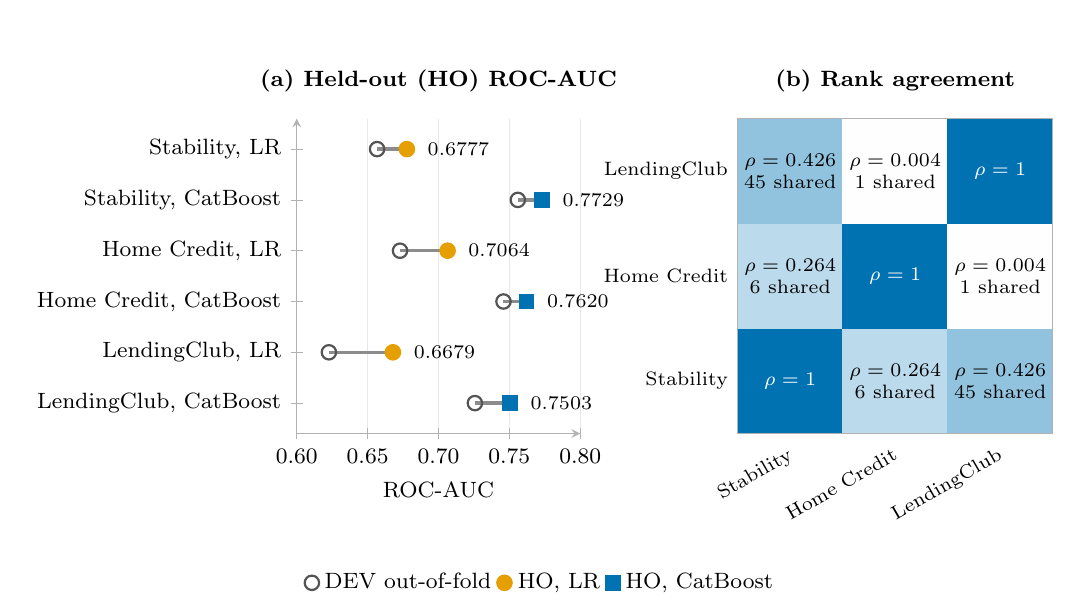
\begin{tikzpicture}
\begin{groupplot}[
    paper,
    group style={group size=2 by 1, horizontal sep=20mm},
    scale only axis, height=4.0cm, clip=false,
]
\nextgroupplot[
    title={(a) Held-out (HO) ROC-AUC},
    width=3.6cm, axis lines=left, xmajorgrids,
    xlabel={ROC-AUC}, xmin=0.60, xmax=0.80, xtick={0.60,0.65,0.70,0.75,0.80},
    xticklabel style={/pgf/number format/fixed, /pgf/number format/precision=2, /pgf/number format/zerofill},
    ymin=0.4, ymax=6.6, ytick={1,2,3,4,5,6},
    yticklabels={{LendingClub, CatBoost},{LendingClub, LR},{Home Credit, CatBoost},{Home Credit, LR},{Stability, CatBoost},{Stability, LR}},
    legend to name=cliplegend, legend columns=3,
]
\addplot[cGrey, line width=1.2pt, forget plot] coordinates {(0.656681,6) (0.677712,6)};
\addplot[cGrey, line width=1.2pt, forget plot] coordinates {(0.755978,5) (0.772872,5)};
\addplot[cGrey, line width=1.2pt, forget plot] coordinates {(0.672869,4) (0.706434,4)};
\addplot[cGrey, line width=1.2pt, forget plot] coordinates {(0.745859,3) (0.761999,3)};
\addplot[cGrey, line width=1.2pt, forget plot] coordinates {(0.622680,2) (0.667862,2)};
\addplot[cGrey, line width=1.2pt, forget plot] coordinates {(0.725691,1) (0.750327,1)};
\addplot[only marks, mark=o, mark size=2.6pt, thick, cGrey!60!black]
    coordinates {(0.656681,6) (0.755978,5) (0.672869,4) (0.745859,3) (0.622680,2) (0.725691,1)};
\addlegendentry{DEV out-of-fold}
\addplot[only marks, mark=*, mark size=2.8pt, cOrange] coordinates {(0.677712,6) (0.706434,4) (0.667862,2)};
\addlegendentry{HO, LR}
\addplot[only marks, mark=square*, mark size=2.6pt, cBlue] coordinates {(0.772872,5) (0.761999,3) (0.750327,1)};
\addlegendentry{HO, CatBoost}
\node[font=\scriptsize, anchor=west, xshift=4pt] at (axis cs:0.6777,6) {0.6777};
\node[font=\scriptsize, anchor=west, xshift=4pt] at (axis cs:0.772872,5) {0.7729};
\node[font=\scriptsize, anchor=west, xshift=4pt] at (axis cs:0.7064,4) {0.7064};
\node[font=\scriptsize, anchor=west, xshift=4pt] at (axis cs:0.761999,3) {0.7620};
\node[font=\scriptsize, anchor=west, xshift=4pt] at (axis cs:0.6679,2) {0.6679};
\node[font=\scriptsize, anchor=west, xshift=4pt] at (axis cs:0.750327,1) {0.7503};
\nextgroupplot[
    title={(b) Rank agreement},
    width=4.0cm,
    xmin=-0.5, xmax=2.5, ymin=-0.5, ymax=2.5,
    xtick={0,1,2}, xticklabels={Stability,Home Credit,LendingClub},
    ytick={0,1,2}, yticklabels={Stability,Home Credit,LendingClub},
    x tick label style={rotate=30, anchor=north east, font=\scriptsize},
    y tick label style={font=\scriptsize},
    tick style={draw=none}, enlargelimits=false, axis on top,
    colormap={paperblue}{color=(white) color=(cBlue)},
    point meta min=0, point meta max=1,
]
\addplot[matrix plot*, mesh/cols=3, point meta=explicit] coordinates {
    (0,0) [1] (1,0) [0.264] (2,0) [0.426]
    (0,1) [0.264] (1,1) [1] (2,1) [0.004]
    (0,2) [0.426] (1,2) [0.004] (2,2) [1]
};
\node[font=\scriptsize, white] at (axis cs:0,0) {$\rho=1$};
\node[font=\scriptsize, white] at (axis cs:1,1) {$\rho=1$};
\node[font=\scriptsize, white] at (axis cs:2,2) {$\rho=1$};
\node[font=\scriptsize, align=center] at (axis cs:1,0) {$\rho=0.264$\\6 shared};
\node[font=\scriptsize, align=center] at (axis cs:0,1) {$\rho=0.264$\\6 shared};
\node[font=\scriptsize, align=center] at (axis cs:2,0) {$\rho=0.426$\\45 shared};
\node[font=\scriptsize, align=center] at (axis cs:0,2) {$\rho=0.426$\\45 shared};
\node[font=\scriptsize, align=center] at (axis cs:2,1) {$\rho=0.004$\\1 shared};
\node[font=\scriptsize, align=center] at (axis cs:1,2) {$\rho=0.004$\\1 shared};
\end{groupplot}
\node[anchor=north, yshift=-2mm] at (current bounding box.south) {\pgfplotslegendfromname{cliplegend}};
\end{tikzpicture}
\caption{CLIP-ranked selection on Stability 2024. (a) Held-out (HO) ROC-AUC of the six source--backbone cells on the earlier Stability cohort; the hollow marker is the pooled DEV out-of-fold AUC, so the grey bar shows the difference between the HO value and the development estimate. (b) Spearman correlation over all 1,959 features between the rankings produced by the three source representations, with the number of features shared by the two top-100 lists; the colour scale runs from 0 (white) to 1 (blue), the diagonal shows the self-correlation of 1, and darker cells indicate closer agreement.}
\label{fig:clip}
\end{figure*}

The three source representations do not produce one universal ordering of the Stability predictors (Figure~\ref{fig:clip}b): the native Stability ranking shares only 6 of its top 100 features with the Home Credit ranking (Spearman $\rho=0.264$) and 45 with the LendingClub ranking ($\rho=0.426$), and Home Credit and LendingClub share a single feature ($\rho=0.004$). Transfer is therefore source-dependent. A possible explanation is that each source carries its own descriptor transform, projection geometry and anchor, so the same features are scored through different coordinate systems; the target-aware redundancy stage and classifier then operate on pools that differ substantially between sources. These cells are separate source--target evaluations: the earlier experiments in which the same sources ranked Home Credit features (0.7627 for the Home Credit source with CatBoost; 0.6766 and 0.5732 for the LendingClub source with CatBoost and logistic regression) concern a different target dataset, so the Stability values (0.7620; 0.7503 and 0.6679) show neither that a representation stayed unchanged nor that it improved. The five native seeds are homogeneous (validation mean reciprocal rank 0.2255 to 0.2651 over 395 held-out pairs, Recall@10 0.472 to 0.546, cosine margin 0.528 to 0.568, all collapse checks passed). Finally, the reason for assessing the branch on reproducibility is visible in its earlier Home Credit evaluation, under the protocol of that version (Table~\ref{tab:stages}): inserting the corrected contrastive ranking between LLM screening and mRMR changed HO AUC by $-0.001102$ (logistic regression) and $+0.000866$ (CatBoost) while raising mean pairwise Jaccard by $+0.324841$ and $+0.498638$; a possible explanation, not tested here, is that the representation imposes a consistent ordering inside a pool that already contains the strong predictors.

\section{Rank voting}
\label{app:voting}
\setcounter{table}{0}\setcounter{figure}{0}

This appendix reports the two rank-voting families in full; they are summarised in Section~\ref{subsec:supplementary_discussion}. The Home Credit family varies pool size and voter set together with the order of combination, so it does not isolate the effect of sequential versus parallel combination.

\subsection{Rank-aggregation method}
\label{subsec:voting_fs}

The voting experiment asks whether the sequential order \emph{LLM then statistical refinement} discards information that a parallel combination would retain. It is run on Home Credit over the candidate set of $d=373$ features. For a feature with rank $r$ in a source ranking (rank 1 best) the normalised rank is
\begin{equation}
    r^{\mathrm{norm}}=\frac{r-1}{d-1},
    \label{eq:normrank}
\end{equation}
so that the best feature maps to 0 and the worst to 1. The two-voter score averages the normalised LLM and contrastive ranks; the top $P\in\{100,200,300\}$ features form a pool that mutual-information mRMR reduces to $\Kfeat=20$ or $40$, with ties resolved by LLM rank, then contrastive rank, then feature name. A \emph{direct three-voter} variant averages the normalised LLM, contrastive and mRMR relevance ranks and selects the top $\Kfeat$ without refinement. The candidate-set LLM ranking was generated from label-free metadata for all 373 features, the contrastive coverage was extended deterministically to 93 features lacking descriptors using the frozen representation and DEV-only descriptors, and the mRMR relevance ranking used DEV labels only. Averaging normalised ranks is a Borda-type rule \cite{dwork2001} in the tradition of ensemble feature selection \cite{saeys2008}. Because the voting variants differ from the sequential pipeline in pool size and in the rankings they combine as well as in the order of combination, the experiment compares particular pipeline configurations and does not isolate the effect of ordering.

A second, pre-declared voting family extends rank aggregation to classical voters on both Home Credit and LendingClub. For each dataset and backbone the normalised ranks of three target-aware selectors fitted on the fold training partition, the RF/correlation mRMR filter, Boruta and RFE, are averaged, the top $P\in\{100,200,300\}$ features form the candidate pool, and the budgeted subset of $\Kfeat$ features is selected from that pool; $P=200$ is the primary configuration and $P=100$ and $P=300$ are sensitivity configurations. The reference is the RF/correlation mRMR filter applied to the whole candidate set of 373 or 675 features under the same backbone. The twelve comparisons, three per dataset--backbone case, were fixed in a protocol file before any held-out result of the family was computed, and Holm correction is applied within each case's family of three AUC tests. This family contains no semantic voter, so it compares aggregated classical rankings with a single classical filter under the same budget and does not bear on the order of semantic and statistical combination.

Inference in the classical voting family uses the two-sided paired DeLong test \cite{delong1988} on identical HO observations, 95\% intervals from 2,000 target-stratified paired bootstrap resamples with seed 20260721, and Holm's step-down procedure \cite{holm1979} within each dataset--backbone family of three pre-declared tests. The Home Credit voting family compares each of the eight voting variants with two comparators, the sequential pipeline LLM then mRMR and full-pool mRMR, and is reported as point differences on the same HO observations. Unlike the descriptive comparisons of Table~\ref{tab:primary_results}, the classical voting family was declared before its held-out results were computed.

\subsection{Results}
\label{subsec:voting_results}

Table~\ref{tab:voting} and Figure~\ref{fig:voting} compare the eight Home Credit voting variants with the sequential pipeline LLM then mRMR that they are designed to improve on, and with full-pool mRMR applied to all 373 candidate features; the comparators are the pipelines of Tables~\ref{tab:full_matrix} and \ref{tab:llm_pipelines} (LLM then mRMR 0.7432 and 0.7758, full-pool mRMR 0.7699 and 0.7599), and this family is reported as point differences. Voting exceeds the sequential comparator in two of eight point estimates, by $+0.0008$ ($P=200$) and $+0.0014$ ($P=300$) with logistic regression, and lies below it in the other six, by 0.0027 to 0.0038 with logistic regression and by 0.0094 to 0.0213 with CatBoost. Among the pool-based variants AUC rises monotonically with the pool size $P$ for both backbones, from 0.7394 at $P=100$ to 0.7447 at $P=300$ for logistic regression and from 0.7588 to 0.7664 for CatBoost, and the direct three-voter selector is weaker than the best pool-based variant under both backbones. Against full-pool mRMR, whose CatBoost reference is the same mutual-information selector as in the headline tables, seven of eight point estimates are negative: the logistic-regression deficits are 0.025 to 0.030, the CatBoost deficits 0.0006 to 0.0054, and CatBoost at $P=300$ is $+0.0065$ above the reference. In terms of AUC, parallel aggregation of the semantic and contrastive rankings therefore does not improve on the sequential pipeline by more than $+0.0014$ and is 0.009 to 0.021 below it with CatBoost; these are AUC differences between particular configurations that differ in pool size and in the rankings combined as well as in ordering, so they neither isolate the effect of sequential versus parallel combination nor measure information recovered.

\begin{table*}[htbp]
\centering
\scriptsize
\setlength{\tabcolsep}{3pt}
\begin{threeparttable}
\caption{Home Credit voting experiment. Pool variants average the normalised LLM and contrastive ranks, keep the top $P$ features and apply mutual-information mRMR; the direct variant averages LLM, contrastive and mRMR relevance ranks and selects $\Kfeat$ directly. $\Delta_{\mathrm{seq}}$ is voting minus the sequential comparator (LLM then mRMR) and $\Delta_{\mathrm{full}}$ voting minus full-pool mRMR on all 373 candidate features, on the same HO observations; the comparators are the pipelines of Tables~\ref{tab:full_matrix} and \ref{tab:llm_pipelines}, and this family is reported as point differences. AUC is shown to four decimals and $\Delta$ at full precision.}
\label{tab:voting}
\begin{tabular}{@{}lrrrrrr@{}}
\toprule
 & \multicolumn{3}{c}{Logistic regression, $\Kfeat=20$} & \multicolumn{3}{c}{CatBoost, $\Kfeat=40$} \\
\cmidrule(lr){2-4}\cmidrule(l){5-7}
Variant & AUC & $\Delta_{\mathrm{seq}}$ & $\Delta_{\mathrm{full}}$ & AUC & $\Delta_{\mathrm{seq}}$ & $\Delta_{\mathrm{full}}$ \\
\midrule
Pool $P=100$, then mRMR & 0.7394 & $-0.003797$ & $-0.030458$ & 0.7588 & $-0.017071$ & $-0.001142$ \\
Pool $P=200$, then mRMR & 0.7440 & $+0.000791$ & $-0.025870$ & 0.7593 & $-0.016565$ & $-0.000636$ \\
Pool $P=300$, then mRMR & 0.7447 & $+0.001424$ & $-0.025237$ & 0.7664 & $-0.009380$ & $+0.006549$ \\
Direct three-voter & 0.7406 & $-0.002656$ & $-0.029317$ & 0.7545 & $-0.021307$ & $-0.005378$ \\
\midrule
Sequential LLM then mRMR & 0.7432 & & & 0.7758 & & \\
Full-pool mRMR (373 features) & 0.7699 & & & 0.7599 & & \\
\bottomrule
\end{tabular}
\end{threeparttable}
\end{table*}

\begin{figure*}[htbp]
\centering
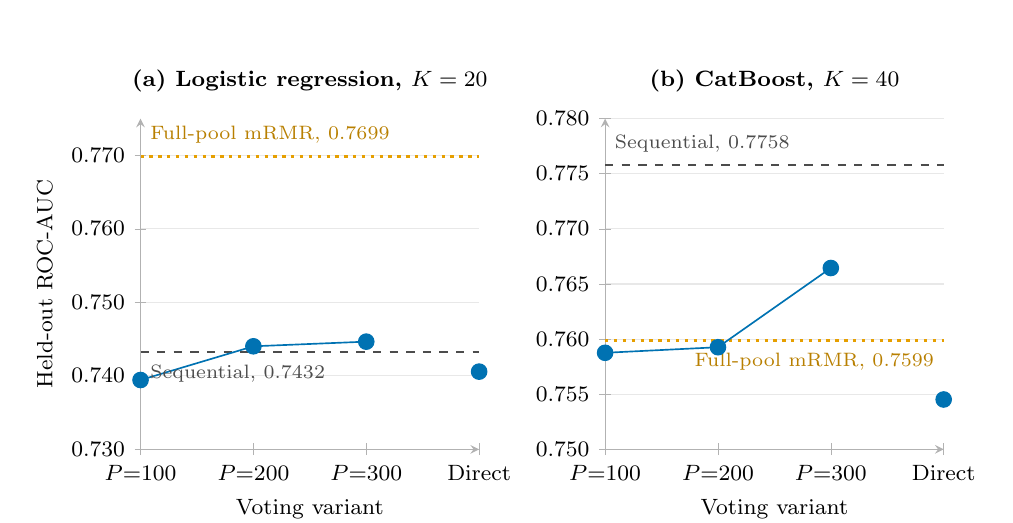
\begin{tikzpicture}
\begin{groupplot}[
    paper,
    group style={group size=2 by 1, horizontal sep=16mm},
    scale only axis, width=4.3cm, height=4.2cm, clip=false,
    symbolic x coords={100,200,300,Direct},
    xtick={100,200,300,Direct}, xticklabels={$P{=}100$,$P{=}200$,$P{=}300$,Direct},
    enlarge x limits=0.22, ymajorgrids, axis lines=left,
    yticklabel style={/pgf/number format/fixed, /pgf/number format/precision=3, /pgf/number format/zerofill},
    xlabel={Voting variant},
]
\nextgroupplot[title={(a) Logistic regression, $\Kfeat=20$}, ylabel={Held-out ROC-AUC}, ymin=0.730, ymax=0.775, ytick distance=0.010]
\addplot[dashed, thick, gray!60!black] coordinates {(100,0.743229) (Direct,0.743229)};
\addplot[dotted, very thick, cOrange] coordinates {(100,0.769890) (Direct,0.769890)};
\addplot[cBlue, semithick, mark=none] coordinates {(100,0.739432) (200,0.744020) (300,0.744653)};
\addplot[only marks, mark=*, mark size=2.8pt, cBlue] coordinates {(100,0.739432) (200,0.744020) (300,0.744653) (Direct,0.740573)};
\node[font=\scriptsize, anchor=north west, gray!60!black] at (axis cs:100,0.743229) [yshift=-1pt] {Sequential, 0.7432};
\node[font=\scriptsize, anchor=south west, cOrange!80!black] at (axis cs:100,0.769890) [yshift=1pt] {Full-pool mRMR, 0.7699};
\nextgroupplot[title={(b) CatBoost, $\Kfeat=40$}, ymin=0.750, ymax=0.780, ytick distance=0.005]
\addplot[dashed, thick, gray!60!black] coordinates {(100,0.775828) (Direct,0.775828)};
\addplot[dotted, very thick, cOrange] coordinates {(100,0.759899) (Direct,0.759899)};
\addplot[cBlue, semithick, mark=none] coordinates {(100,0.758757) (200,0.759263) (300,0.766448)};
\addplot[only marks, mark=*, mark size=2.8pt, cBlue] coordinates {(100,0.758757) (200,0.759263) (300,0.766448) (Direct,0.754521)};
\node[font=\scriptsize, anchor=south west, gray!60!black] at (axis cs:100,0.775828) [yshift=1pt] {Sequential, 0.7758};
\node[font=\scriptsize, anchor=north east, cOrange!80!black] at (axis cs:Direct,0.759899) [yshift=-1pt] {Full-pool mRMR, 0.7599};
\end{groupplot}
\end{tikzpicture}
\caption{Home Credit voting AUC by candidate-pool size for (a) logistic regression and (b) CatBoost. The dashed line is the sequential comparator LLM then mRMR and the dotted line full-pool mRMR on all 373 candidate features, both at the values of Tables~\ref{tab:full_matrix} and \ref{tab:llm_pipelines}. The vertical scales differ between panels.}
\label{fig:voting}
\end{figure*}

A second voting family, pre-declared and run on both Home Credit and LendingClub, aggregates three classical rankings (RF/correlation mRMR, Boruta and RFE) and compares the result with the RF/correlation mRMR filter applied to the whole candidate set (\ref{subsec:voting_fs}). Table~\ref{tab:voting_cross} reports the twelve comparisons. Every point estimate is positive and every difference is Holm-significant within its family of three tests, with 95\% bootstrap intervals that exclude zero in all twelve cases; the gains range from $+0.0020$ (Home Credit logistic regression, $P=300$) to $+0.0129$ (LendingClub CatBoost, $P=300$), and KS moves in the same direction as AUC in every comparison. On Home Credit the CatBoost gains ($+0.0088$ to $+0.0100$) exceed the logistic-regression gains ($+0.0020$ to $+0.0045$), and in three of the four cases the largest gain occurs at $P=300$. The reference values of this family (0.7448, 0.7698, 0.6915 and 0.7072) are those of the RF/correlation implementation and differ from the mutual-information mRMR values of Table~\ref{tab:primary_results}, so the two voting families are not compared with each other. The result shows that aggregating classical rankings over a wider pool raised held-out AUC over a single classical filter on both datasets; the voting variants and the reference differ in pool construction as well as in aggregation, so the comparison is again between configurations. Fold-to-fold reproducibility of the voted subsets was lower than that of the reference filter in every case (mean fold Jaccard 0.40 to 0.49 against 0.62 to 0.72).

\begin{table*}[htbp]
\centering
\scriptsize
\setlength{\tabcolsep}{4pt}
\begin{threeparttable}
\caption{Cross-dataset classical voting family. Voting averages the normalised RF/correlation mRMR, Boruta and RFE ranks, keeps the top $P$ features and selects $\Kfeat=20$ (LR) or $40$ (CatBoost) from that pool; the reference is RF/correlation mRMR on the whole candidate set. $\Delta$ is voting minus reference on paired HO observations (120,053 Home Credit; 293,105 LendingClub); the interval is the 95\% paired percentile bootstrap (2,000 resamples); $p$-values are Holm-adjusted within each dataset--backbone family of three AUC tests.}
\label{tab:voting_cross}
\begin{tabular}{@{}llrrrlrr@{}}
\toprule
Case & Pool $P$ & Ref.\ AUC & Voting AUC & $\Delta$AUC & 95\% CI & Holm $p$ & $\Delta$KS \\
\midrule
Home Credit, LR & 100 & 0.7448 & 0.7493 & $+0.0045$ & $[0.0026,\,0.0065]$ & $2.0\times10^{-5}$ & $+0.0071$ \\
 & 200 (primary) & 0.7448 & 0.7492 & $+0.0045$ & $[0.0025,\,0.0064]$ & $3.2\times10^{-5}$ & $+0.0108$ \\
 & 300 & 0.7448 & 0.7467 & $+0.0020$ & $[0.0002,\,0.0038]$ & 0.031 & $+0.0090$ \\
\addlinespace
Home Credit, CatBoost & 100 & 0.7698 & 0.7791 & $+0.0093$ & $[0.0077,\,0.0109]$ & $<10^{-10}$ & $+0.0127$ \\
 & 200 (primary) & 0.7698 & 0.7786 & $+0.0088$ & $[0.0070,\,0.0105]$ & $<10^{-10}$ & $+0.0113$ \\
 & 300 & 0.7698 & 0.7799 & $+0.0100$ & $[0.0082,\,0.0119]$ & $<10^{-10}$ & $+0.0127$ \\
\addlinespace
LendingClub v2, LR & 100 & 0.6915 & 0.6977 & $+0.0062$ & $[0.0055,\,0.0069]$ & $<10^{-10}$ & $+0.0086$ \\
 & 200 (primary) & 0.6915 & 0.6951 & $+0.0036$ & $[0.0030,\,0.0041]$ & $<10^{-10}$ & $+0.0063$ \\
 & 300 & 0.6915 & 0.6990 & $+0.0075$ & $[0.0067,\,0.0082]$ & $<10^{-10}$ & $+0.0116$ \\
\addlinespace
LendingClub v2, CatBoost & 100 & 0.7072 & 0.7140 & $+0.0068$ & $[0.0062,\,0.0074]$ & $<10^{-10}$ & $+0.0097$ \\
 & 200 (primary) & 0.7072 & 0.7173 & $+0.0101$ & $[0.0095,\,0.0108]$ & $<10^{-10}$ & $+0.0156$ \\
 & 300 & 0.7072 & 0.7201 & $+0.0129$ & $[0.0122,\,0.0136]$ & $<10^{-10}$ & $+0.0202$ \\
\bottomrule
\end{tabular}
\end{threeparttable}
\end{table*}

\section{Feature-budget sensitivity}
\label{app:budgets}
\setcounter{table}{0}\setcounter{figure}{0}

This appendix reports the development evidence behind the budgets fixed in Section~\ref{subsec:feature_budgets}. Every selector of Table~\ref{tab:methods} was refitted at $\Kfeat \in \{10,20,30,40,50\}$ on the five development folds of each dataset, and the mean fold AUC is recorded; no held-out observation enters this appendix, and the values are development quantities that describe a design decision rather than a reported result. At the documented budgets the values are the same development means that select the family leaders of Table~\ref{tab:confirmatory}.

Figure~\ref{fig:budgets}a gives the mean development AUC of all selectors of a backbone relative to its documented budget. Logistic regression gains $+0.004$ at $\Kfeat=30$ and $+0.005$ at $\Kfeat=40$ over $\Kfeat=20$ and flattens thereafter, so the linear budget trades a small amount of development discrimination for half the feature count; CatBoost rises to $\Kfeat=40$ and gains nothing beyond it ($-0.0005$ at $\Kfeat=50$). The budget applies identically to every selector of a case, so it moves their common level and not their relative position.

Figure~\ref{fig:budgets}b and Table~\ref{tab:budgets} give the quantity that matters for RQ1, the development AUC of the LLM-assisted family leader minus that of the classical family leader, at each budget. The sign is the same at all five budgets in five of the six cases, and in the sixth, Stability 2024 with logistic regression, only the smallest budget $\Kfeat=10$ differs. The margin does not narrow as the budget grows: on LendingClub v2 with logistic regression it widens from $+0.0150$ at $\Kfeat=10$ to $+0.0259$ at $\Kfeat=50$. Both backbones are evaluated at every budget from $\Kfeat=10$ to $\Kfeat=50$; at $\Kfeat=30$ all six signs agree with the documented budgets, so the two backbones can be compared at equal subset size without changing any conclusion. These are development comparisons; the held-out results of Tables~\ref{tab:primary_results} and \ref{tab:confirmatory} are unaffected by this appendix, which bears only on whether the fixed budgets favoured one family.

The same curves separate the two factors that differ between the backbones. At equal budget CatBoost exceeds logistic regression by $+0.020$ to $+0.037$ mean development AUC at $\Kfeat=40$ and by $+0.015$ to $+0.037$ at every budget from 10 to 50 features, in all three datasets; selector by selector the ordering holds in all fourteen cases on Home Credit and Stability 2024 and in ten to twelve of fourteen on LendingClub v2. Against the unmatched difference produced by the reported budgets ($+0.025$ to $+0.042$), the budget accounts for 11 to 24 per cent of the gap and the model class for the remainder. This is a development comparison; no held-out model was refitted at a matched budget.

\begin{figure*}[htbp]
\centering
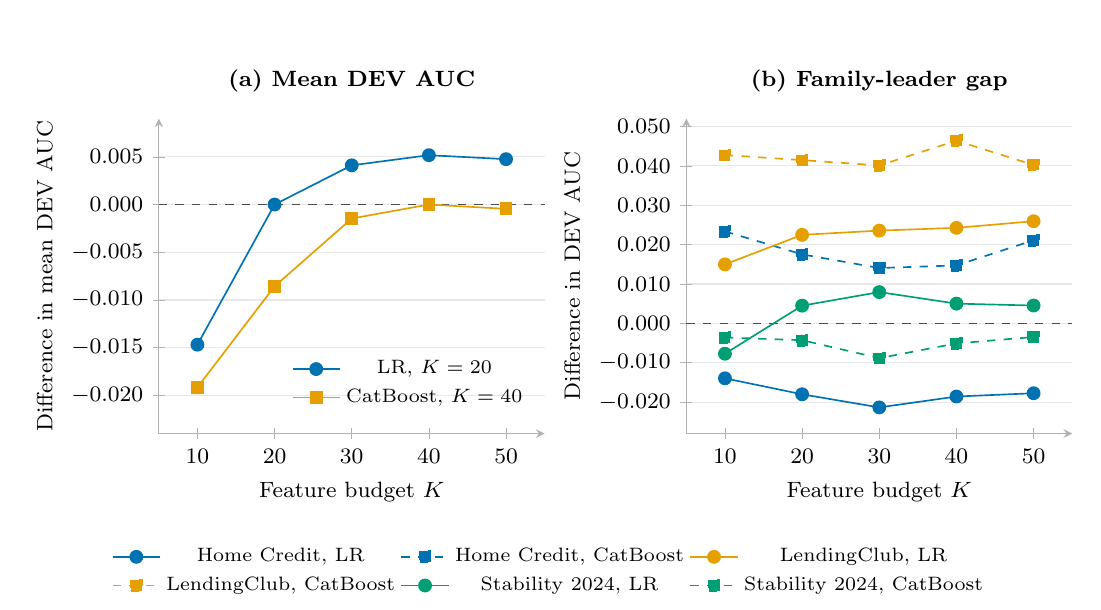
\begin{tikzpicture}
\begin{groupplot}[
    paper,
    group style={group size=2 by 1, horizontal sep=18mm},
    scale only axis, width=4.9cm, height=4.0cm, clip=false,
    xmin=5, xmax=55, xtick={10,20,30,40,50},
    xlabel={Feature budget $\Kfeat$},
    ymajorgrids, axis lines=left,
    yticklabel style={/pgf/number format/fixed, /pgf/number format/precision=3, /pgf/number format/zerofill},
]
\nextgroupplot[title={(a) Mean DEV AUC}, ylabel={Difference in mean DEV AUC}, ymin=-0.024, ymax=0.009, ytick={-0.02,-0.015,-0.01,-0.005,0,0.005},
    legend style={at={(0.98,0.05)}, anchor=south east, draw=none, fill=none, font=\scriptsize}]
\draw[gray!60!black, dashed] (axis cs:5,0) -- (axis cs:55,0);
\addplot[cBlue, semithick, mark=*, mark size=2.2pt] coordinates {(10,-0.014685) (20,0.000000) (30,0.004107) (40,0.005168) (50,0.004752)};
\addlegendentry{LR, $\Kfeat=20$}
\addplot[cOrange, semithick, mark=square*, mark size=2.0pt] coordinates {(10,-0.019158) (20,-0.008574) (30,-0.001466) (40,0.000000) (50,-0.000453)};
\addlegendentry{CatBoost, $\Kfeat=40$}
\nextgroupplot[title={(b) Family-leader gap}, ylabel={Difference in DEV AUC}, ymin=-0.028, ymax=0.052, ytick={-0.02,-0.01,0,0.01,0.02,0.03,0.04,0.05},
    legend to name=budgetlegend, legend columns=3, legend style={draw=none, fill=none, font=\scriptsize}]
\draw[gray!60!black, dashed] (axis cs:5,0) -- (axis cs:55,0);
\addplot[cBlue, semithick, mark=*, mark size=2.2pt] coordinates {(10,-0.013960) (20,-0.018022) (30,-0.021352) (40,-0.018588) (50,-0.017754)};
\addlegendentry{Home Credit, LR}
\addplot[cBlue, semithick, dashed, mark=square*, mark size=2.0pt] coordinates {(10,0.023343) (20,0.017522) (30,0.014054) (40,0.014717) (50,0.021106)};
\addlegendentry{Home Credit, CatBoost}
\addplot[cOrange, semithick, mark=*, mark size=2.2pt] coordinates {(10,0.014980) (20,0.022480) (30,0.023558) (40,0.024256) (50,0.025945)};
\addlegendentry{LendingClub, LR}
\addplot[cOrange, semithick, dashed, mark=square*, mark size=2.0pt] coordinates {(10,0.042744) (20,0.041458) (30,0.040106) (40,0.046391) (50,0.040232)};
\addlegendentry{LendingClub, CatBoost}
\addplot[cGreen, semithick, mark=*, mark size=2.2pt] coordinates {(10,-0.007712) (20,0.004491) (30,0.007940) (40,0.005008) (50,0.004522)};
\addlegendentry{Stability 2024, LR}
\addplot[cGreen, semithick, dashed, mark=square*, mark size=2.0pt] coordinates {(10,-0.003589) (20,-0.004279) (30,-0.008830) (40,-0.005092) (50,-0.003468)};
\addlegendentry{Stability 2024, CatBoost}
\end{groupplot}
\node[anchor=north, yshift=-2mm] at (current bounding box.south) {\pgfplotslegendfromname{budgetlegend}};
\end{tikzpicture}
\caption{Feature-budget sensitivity on development data. (a) Mean development AUC of all selectors of a backbone at each budget, measured against that backbone's documented budget (logistic regression $\Kfeat=20$, CatBoost $\Kfeat=40$; zero by construction at those points). (b) Development AUC of the LLM-assisted family leader minus that of the classical family leader, in each dataset--backbone case; positive values favour LLM-assisted selection. Circles and solid lines are logistic regression, squares and dashed lines CatBoost. No held-out observation enters either panel.}
\label{fig:budgets}
\end{figure*}

\begin{table*}[htbp]
\centering
\footnotesize
\begin{threeparttable}
\caption{Development AUC of the LLM-assisted family leader minus that of the classical family leader, by feature budget; the values plotted in Figure~\ref{fig:budgets}b. Bold marks the documented budget of the backbone. Positive values favour LLM-assisted selection.}
\label{tab:budgets}
\setlength{\tabcolsep}{4pt}
\begin{tabular}{@{}lrrrrr@{}}
\toprule
Case & \multicolumn{5}{c}{Feature budget $\Kfeat$} \\
\cmidrule(l){2-6}
 & 10 & 20 & 30 & 40 & 50 \\
\midrule
Home Credit, LR & $-0.0140$ & $\mathbf{-0.0180}$ & $-0.0214$ & $-0.0186$ & $-0.0178$ \\
Home Credit, CatBoost & $+0.0233$ & $+0.0175$ & $+0.0141$ & $\mathbf{+0.0147}$ & $+0.0211$ \\
LendingClub v2, LR & $+0.0150$ & $\mathbf{+0.0225}$ & $+0.0236$ & $+0.0243$ & $+0.0259$ \\
LendingClub v2, CatBoost & $+0.0427$ & $+0.0415$ & $+0.0401$ & $\mathbf{+0.0464}$ & $+0.0402$ \\
Stability 2024, LR & $-0.0077$ & $\mathbf{+0.0045}$ & $+0.0079$ & $+0.0050$ & $+0.0045$ \\
Stability 2024, CatBoost & $-0.0036$ & $-0.0043$ & $-0.0088$ & $\mathbf{-0.0051}$ & $-0.0035$ \\
\bottomrule
\end{tabular}
\end{threeparttable}
\end{table*}


\section{Headline subsets}
\label{app:subsets}
\setcounter{table}{0}\setcounter{figure}{0}

This appendix lists the twelve subsets behind Table~\ref{tab:primary_results}: for each dataset--backbone case, the features selected by the frozen full-DEV refit of the LLM-assisted family leader and of the classical family leader, in the order the selector produced them ($\Kfeat=20$ for logistic regression, $\Kfeat=40$ for CatBoost). Each dataset takes two tables: the first gives ranks 1 to 20 of all four subsets, the second ranks 21 to 40 of the two CatBoost subsets. For pure LLM the order is that of the cached full-DEV ranking; on Stability 2024 one ranking served both backbones, so its logistic-regression subset is the first twenty names of its CatBoost subset. Feature names are those of the engineered universes of Section~\ref{subsec:datasets}; on Home Credit the three external scores occupy the first three ranks of the pure LLM list, as noted in Section~\ref{subsec:stability_results}. The lists are provided as \texttt{headline\_subsets.csv} in the repository.

\begin{table*}[htbp]
\centering
\scriptsize
\begin{threeparttable}
\caption{Home Credit, ranks 1 to 20: full-DEV subsets of the two family leaders under each backbone (Table~\ref{tab:primary_results}), in selector order. The two logistic-regression subsets share 4 of 20 features; the two CatBoost subsets share 16 of 40 (continued in Table~\ref{tab:subsets_homecredit_b}).}
\label{tab:subsets_homecredit}
\setlength{\tabcolsep}{3pt}
\renewcommand{\arraystretch}{0.9}
\begin{tabular}{@{}rL{40mm}L{40mm}L{40mm}L{40mm}@{}}
\toprule
Rank & LR: Stable core + LLM fill (LLM-assisted) & LR: mRMR (classical) & CatBoost: Pure LLM (LLM-assisted) & CatBoost: RFE CatBoost (classical) \\
\midrule
1 & \texttt{EXT\_\allowbreak SOURCE\_\allowbreak 2} & \texttt{EXT\_\allowbreak SOURCE\_\allowbreak 3} & \texttt{EXT\_\allowbreak SOURCE\_\allowbreak 3} & \texttt{EXT\_\allowbreak SOURCE\_\allowbreak 2} \\
2 & \texttt{EXT\_\allowbreak SOURCE\_\allowbreak 3} & \texttt{EXT\_\allowbreak SOURCE\_\allowbreak 2} & \texttt{EXT\_\allowbreak SOURCE\_\allowbreak 2} & \texttt{EXT\_\allowbreak SOURCE\_\allowbreak 3} \\
3 & \texttt{PREV\_\allowbreak INTEREST\_\allowbreak ESTIMATE\_\allowbreak MAX} & \texttt{CODE\_\allowbreak GENDER} & \texttt{EXT\_\allowbreak SOURCE\_\allowbreak 1} & \texttt{EXT\_\allowbreak SOURCE\_\allowbreak 1} \\
4 & \texttt{EXT\_\allowbreak SOURCE\_\allowbreak 1} & \texttt{CC\_\allowbreak CNT\_\allowbreak DRAWINGS\_\allowbreak ATM\_\allowbreak CURRENT\_\allowbreak MEAN} & \texttt{DAYS\_\allowbreak BIRTH} & \texttt{PREV\_\allowbreak INTEREST\_\allowbreak ESTIMATE\_\allowbreak MAX} \\
5 & \texttt{DAYS\_\allowbreak EMPLOYED} & \texttt{POS\_\allowbreak LATE\_\allowbreak PAYMENT\_\allowbreak MEAN} & \texttt{DAYS\_\allowbreak EMPLOYED} & \texttt{DAYS\_\allowbreak BIRTH} \\
6 & \texttt{BURO\_\allowbreak DEBT\_\allowbreak CREDIT\_\allowbreak DIFF\_\allowbreak MIN} & \texttt{DEF\_\allowbreak 30\_\allowbreak CNT\_\allowbreak SOCIAL\_\allowbreak CIRCLE} & \texttt{OCCUPATION\_\allowbreak TYPE} & \texttt{INSTAL\_\allowbreak AMT\_\allowbreak PAYMENT\_\allowbreak SUM} \\
7 & \texttt{INSTAL\_\allowbreak IS\_\allowbreak LATE\_\allowbreak MEAN} & \texttt{PREV\_\allowbreak AMT\_\allowbreak DOWN\_\allowbreak PAYMENT\_\allowbreak SUM} & \texttt{NAME\_\allowbreak INCOME\_\allowbreak TYPE} & \texttt{INSTAL\_\allowbreak IS\_\allowbreak LATE\_\allowbreak MEAN} \\
8 & \texttt{INSTAL\_\allowbreak PAYMENT\_\allowbreak DIFF\_\allowbreak MEAN} & \texttt{FLAG\_\allowbreak WORK\_\allowbreak PHONE} & \texttt{NAME\_\allowbreak EDUCATION\_\allowbreak TYPE} & \texttt{DAYS\_\allowbreak EMPLOYED} \\
9 & \texttt{PREV\_\allowbreak INTEREST\_\allowbreak ESTIMATE\_\allowbreak VAR} & \texttt{BURO\_\allowbreak AMT\_\allowbreak CREDIT\_\allowbreak SUM\_\allowbreak LIMIT\_\allowbreak MIN} & \texttt{NAME\_\allowbreak FAMILY\_\allowbreak STATUS} & \texttt{AMT\_\allowbreak CREDIT} \\
10 & \texttt{DAYS\_\allowbreak REGISTRATION} & \texttt{CC\_\allowbreak AMT\_\allowbreak DRAWINGS\_\allowbreak ATM\_\allowbreak CURRENT\_\allowbreak MIN} & \texttt{CODE\_\allowbreak GENDER} & \texttt{AMT\_\allowbreak ANNUITY} \\
11 & \texttt{POS\_\allowbreak SK\_\allowbreak DPD\_\allowbreak DEF\_\allowbreak MEAN} & \texttt{EXT\_\allowbreak SOURCE\_\allowbreak 1} & \texttt{AMT\_\allowbreak CREDIT} & \texttt{AMT\_\allowbreak GOODS\_\allowbreak PRICE} \\
12 & \texttt{BURO\_\allowbreak DEBT\_\allowbreak CREDIT\_\allowbreak DIFF\_\allowbreak MEAN} & \texttt{PREV\_\allowbreak RATE\_\allowbreak INTEREST\_\allowbreak PRIMARY\_\allowbreak VAR} & \texttt{AMT\_\allowbreak GOODS\_\allowbreak PRICE} & \texttt{INSTAL\_\allowbreak DAYS\_\allowbreak DIFF\_\allowbreak MAX} \\
13 & \texttt{PREV\_\allowbreak INTEREST\_\allowbreak ESTIMATE\_\allowbreak MEAN} & \texttt{WEEKDAY\_\allowbreak APPR\_\allowbreak PROCESS\_\allowbreak START} & \texttt{AMT\_\allowbreak ANNUITY} & \texttt{PREV\_\allowbreak DAYS\_\allowbreak FIRST\_\allowbreak DUE\_\allowbreak SUM} \\
14 & \texttt{CC\_\allowbreak CNT\_\allowbreak DRAWINGS\_\allowbreak ATM\_\allowbreak CURRENT\_\allowbreak MEAN} & \texttt{PREV\_\allowbreak DAYS\_\allowbreak FIRST\_\allowbreak DRAWING\_\allowbreak VAR} & \texttt{BURO\_\allowbreak DEBT\_\allowbreak RATIO\_\allowbreak MAX} & \texttt{CODE\_\allowbreak GENDER} \\
15 & \texttt{DAYS\_\allowbreak BIRTH} & \texttt{COMMONAREA\_\allowbreak AVG} & \texttt{BURO\_\allowbreak DEBT\_\allowbreak RATIO\_\allowbreak MEAN} & \texttt{BURO\_\allowbreak DEBT\_\allowbreak RATIO\_\allowbreak SUM} \\
16 & \texttt{AMT\_\allowbreak CREDIT} & \texttt{FLAG\_\allowbreak CONT\_\allowbreak MOBILE} & \texttt{BURO\_\allowbreak DAYS\_\allowbreak CREDIT\_\allowbreak MEAN} & \texttt{BURO\_\allowbreak DEBT\_\allowbreak RATIO\_\allowbreak MAX} \\
17 & \texttt{AMT\_\allowbreak GOODS\_\allowbreak PRICE} & \texttt{FLAG\_\allowbreak DOCUMENT\_\allowbreak 3} & \texttt{BURO\_\allowbreak DAYS\_\allowbreak CREDIT\_\allowbreak UPDATE\_\allowbreak MEAN} & \texttt{INSTAL\_\allowbreak DAYS\_\allowbreak INSTALMENT\_\allowbreak VAR} \\
18 & \texttt{AMT\_\allowbreak ANNUITY} & \texttt{PREV\_\allowbreak NFLAG\_\allowbreak LAST\_\allowbreak APPL\_\allowbreak IN\_\allowbreak DAY\_\allowbreak MEAN} & \texttt{BURO\_\allowbreak DAYS\_\allowbreak CREDIT\_\allowbreak ENDDATE\_\allowbreak MEAN} & \texttt{PREV\_\allowbreak APPLICATION\_\allowbreak DIFF\_\allowbreak MAX} \\
19 & \texttt{BURO\_\allowbreak DEBT\_\allowbreak RATIO\_\allowbreak MAX} & \texttt{AMT\_\allowbreak REQ\_\allowbreak CREDIT\_\allowbreak BUREAU\_\allowbreak QRT} & \texttt{BURO\_\allowbreak DAYS\_\allowbreak CREDIT\_\allowbreak MAX} & \texttt{PREV\_\allowbreak DAYS\_\allowbreak LAST\_\allowbreak DUE\_\allowbreak 1ST\_\allowbreak VERSION\_\allowbreak MAX} \\
20 & \texttt{BURO\_\allowbreak DEBT\_\allowbreak RATIO\_\allowbreak MEAN} & \texttt{NAME\_\allowbreak HOUSING\_\allowbreak TYPE} & \texttt{BURO\_\allowbreak DAYS\_\allowbreak CREDIT\_\allowbreak MIN} & \texttt{BURO\_\allowbreak DAYS\_\allowbreak CREDIT\_\allowbreak ENDDATE\_\allowbreak MAX} \\
\bottomrule
\end{tabular}
\end{threeparttable}
\end{table*}

\begin{table*}[htbp]
\centering
\scriptsize
\begin{threeparttable}
\caption{Home Credit, ranks 21 to 40 of the two CatBoost subsets of Table~\ref{tab:subsets_homecredit}.}
\label{tab:subsets_homecredit_b}
\setlength{\tabcolsep}{3pt}
\renewcommand{\arraystretch}{0.9}
\begin{tabular}{@{}rL{80mm}L{80mm}@{}}
\toprule
Rank & CatBoost: Pure LLM (LLM-assisted) & CatBoost: RFE CatBoost (classical) \\
\midrule
21 & \texttt{BURO\_\allowbreak DAYS\_\allowbreak ENDDATE\_\allowbreak FACT\_\allowbreak MEAN} & \texttt{NAME\_\allowbreak EDUCATION\_\allowbreak TYPE} \\
22 & \texttt{BURO\_\allowbreak DEBT\_\allowbreak CREDIT\_\allowbreak DIFF\_\allowbreak MEAN} & \texttt{BURO\_\allowbreak DEBT\_\allowbreak CREDIT\_\allowbreak DIFF\_\allowbreak SUM} \\
23 & \texttt{BURO\_\allowbreak DEBT\_\allowbreak RATIO\_\allowbreak VAR} & \texttt{INSTAL\_\allowbreak PAYMENT\_\allowbreak RATIO\_\allowbreak MEAN} \\
24 & \texttt{BURO\_\allowbreak AMT\_\allowbreak CREDIT\_\allowbreak SUM\_\allowbreak DEBT\_\allowbreak MEAN} & \texttt{BURO\_\allowbreak AMT\_\allowbreak CREDIT\_\allowbreak SUM\_\allowbreak MAX} \\
25 & \texttt{BURO\_\allowbreak AMT\_\allowbreak CREDIT\_\allowbreak SUM\_\allowbreak DEBT\_\allowbreak SUM} & \texttt{CC\_\allowbreak LIMIT\_\allowbreak USE\_\allowbreak MEAN} \\
26 & \texttt{BURO\_\allowbreak AMT\_\allowbreak CREDIT\_\allowbreak SUM\_\allowbreak LIMIT\_\allowbreak MEAN} & \texttt{PREV\_\allowbreak INTEREST\_\allowbreak ESTIMATE\_\allowbreak SUM} \\
27 & \texttt{BURO\_\allowbreak AMT\_\allowbreak CREDIT\_\allowbreak SUM\_\allowbreak LIMIT\_\allowbreak SUM} & \texttt{INSTAL\_\allowbreak AMT\_\allowbreak PAYMENT\_\allowbreak MAX} \\
28 & \texttt{BURO\_\allowbreak AMT\_\allowbreak CREDIT\_\allowbreak SUM\_\allowbreak DEBT\_\allowbreak VAR} & \texttt{BURO\_\allowbreak DAYS\_\allowbreak CREDIT\_\allowbreak MEAN} \\
29 & \texttt{BURO\_\allowbreak DAYS\_\allowbreak CREDIT\_\allowbreak UPDATE\_\allowbreak MAX} & \texttt{DAYS\_\allowbreak REGISTRATION} \\
30 & \texttt{BURO\_\allowbreak DAYS\_\allowbreak CREDIT\_\allowbreak ENDDATE\_\allowbreak MAX} & \texttt{CC\_\allowbreak CNT\_\allowbreak DRAWINGS\_\allowbreak CURRENT\_\allowbreak VAR} \\
31 & \texttt{BURO\_\allowbreak DAYS\_\allowbreak CREDIT\_\allowbreak UPDATE\_\allowbreak VAR} & \texttt{REGION\_\allowbreak POPULATION\_\allowbreak RELATIVE} \\
32 & \texttt{BURO\_\allowbreak DAYS\_\allowbreak CREDIT\_\allowbreak VAR} & \texttt{POS\_\allowbreak TOTAL\_\allowbreak INSTALMENT\_\allowbreak PROG\_\allowbreak MEAN} \\
33 & \texttt{BURO\_\allowbreak CREDIT\_\allowbreak DURATION\_\allowbreak MEAN} & \texttt{PREV\_\allowbreak DAYS\_\allowbreak LAST\_\allowbreak DUE\_\allowbreak MAX} \\
34 & \texttt{BURO\_\allowbreak CREDIT\_\allowbreak DURATION\_\allowbreak MAX} & \texttt{CC\_\allowbreak CNT\_\allowbreak DRAWINGS\_\allowbreak ATM\_\allowbreak CURRENT\_\allowbreak MEAN} \\
35 & \texttt{BURO\_\allowbreak CREDIT\_\allowbreak DURATION\_\allowbreak VAR} & \texttt{DAYS\_\allowbreak ID\_\allowbreak PUBLISH} \\
36 & \texttt{BURO\_\allowbreak AMT\_\allowbreak ANNUITY\_\allowbreak SUM} & \texttt{BURO\_\allowbreak DEBT\_\allowbreak RATIO\_\allowbreak MEAN} \\
37 & \texttt{BURO\_\allowbreak CNT\_\allowbreak CREDIT\_\allowbreak PROLONG\_\allowbreak MEAN} & \texttt{INSTAL\_\allowbreak PAYMENT\_\allowbreak DIFF\_\allowbreak MAX} \\
38 & \texttt{BURO\_\allowbreak CNT\_\allowbreak CREDIT\_\allowbreak PROLONG\_\allowbreak MAX} & \texttt{OWN\_\allowbreak CAR\_\allowbreak AGE} \\
39 & \texttt{BURO\_\allowbreak CNT\_\allowbreak CREDIT\_\allowbreak PROLONG\_\allowbreak SUM} & \texttt{NAME\_\allowbreak FAMILY\_\allowbreak STATUS} \\
40 & \texttt{INSTAL\_\allowbreak PAYMENT\_\allowbreak RATIO\_\allowbreak MEAN} & \texttt{BURO\_\allowbreak DEBT\_\allowbreak CREDIT\_\allowbreak DIFF\_\allowbreak MIN} \\
\bottomrule
\end{tabular}
\end{threeparttable}
\end{table*}

\begin{table*}[htbp]
\centering
\scriptsize
\begin{threeparttable}
\caption{LendingClub v2, ranks 1 to 20: full-DEV subsets of the two family leaders under each backbone (Table~\ref{tab:primary_results}), in selector order. The two logistic-regression subsets share 4 of 20 features; the two CatBoost subsets share 21 of 40 (continued in Table~\ref{tab:subsets_lendingclub_b}).}
\label{tab:subsets_lendingclub}
\setlength{\tabcolsep}{3pt}
\renewcommand{\arraystretch}{0.9}
\begin{tabular}{@{}rL{40mm}L{40mm}L{40mm}L{40mm}@{}}
\toprule
Rank & LR: Pure LLM (LLM-assisted) & LR: IV then Boruta (classical) & CatBoost: LLM then mRMR (LLM-assisted) & CatBoost: IV then Boruta (classical) \\
\midrule
1 & \texttt{fico\_\allowbreak mean} & \texttt{term\_\allowbreak home\_\allowbreak ownership} & \texttt{term\_\allowbreak 60 months} & \texttt{term\_\allowbreak home\_\allowbreak ownership} \\
2 & \texttt{fico\_\allowbreak band} & \texttt{term\_\allowbreak verification\_\allowbreak status} & \texttt{acc\_\allowbreak open\_\allowbreak past\_\allowbreak 24mths\_\allowbreak share} & \texttt{term\_\allowbreak verification\_\allowbreak status} \\
3 & \texttt{loan\_\allowbreak to\_\allowbreak income} & \texttt{term} & \texttt{dti} & \texttt{term} \\
4 & \texttt{dti} & \texttt{term\_\allowbreak months} & \texttt{fico\_\allowbreak mean} & \texttt{term\_\allowbreak months} \\
5 & \texttt{annual\_\allowbreak inc} & \texttt{term\_\allowbreak x\_\allowbreak loan\_\allowbreak to\_\allowbreak income} & \texttt{term\_\allowbreak 36 months} & \texttt{term\_\allowbreak x\_\allowbreak loan\_\allowbreak to\_\allowbreak income} \\
6 & \texttt{loan\_\allowbreak amnt} & \texttt{fico\_\allowbreak band\_\allowbreak x\_\allowbreak term} & \texttt{term\_\allowbreak home\_\allowbreak ownership\_\allowbreak 60 months\_\allowbreak \_\allowbreak RENT} & \texttt{fico\_\allowbreak band\_\allowbreak x\_\allowbreak term} \\
7 & \texttt{term} & \texttt{loan\_\allowbreak amnt\_\allowbreak to\_\allowbreak income} & \texttt{term\_\allowbreak x\_\allowbreak loan\_\allowbreak to\_\allowbreak income} & \texttt{loan\_\allowbreak amnt\_\allowbreak to\_\allowbreak income} \\
8 & \texttt{home\_\allowbreak ownership} & \texttt{loan\_\allowbreak to\_\allowbreak income} & \texttt{fico\_\allowbreak band\_\allowbreak x\_\allowbreak term\_\allowbreak near\_\allowbreak prime\_\allowbreak \_\allowbreak 60 months} & \texttt{loan\_\allowbreak to\_\allowbreak income} \\
9 & \texttt{verification\_\allowbreak status} & \texttt{loan\_\allowbreak to\_\allowbreak income\_\allowbreak x\_\allowbreak fico} & \texttt{acc\_\allowbreak open\_\allowbreak past\_\allowbreak 24mths\_\allowbreak per\_\allowbreak total\_\allowbreak acc} & \texttt{loan\_\allowbreak to\_\allowbreak income\_\allowbreak x\_\allowbreak fico} \\
10 & \texttt{purpose} & \texttt{fico\_\allowbreak mean} & \texttt{term\_\allowbreak home\_\allowbreak ownership\_\allowbreak 36 months\_\allowbreak \_\allowbreak MORTGAGE} & \texttt{fico\_\allowbreak mean} \\
11 & \texttt{total\_\allowbreak bc\_\allowbreak limit} & \texttt{fico\_\allowbreak midpoint\_\allowbreak scaled} & \texttt{fico\_\allowbreak range\_\allowbreak high} & \texttt{fico\_\allowbreak midpoint\_\allowbreak scaled} \\
12 & \texttt{bc\_\allowbreak open\_\allowbreak to\_\allowbreak buy} & \texttt{fico\_\allowbreak range\_\allowbreak high} & \texttt{term\_\allowbreak verification\_\allowbreak status\_\allowbreak 60 months\_\allowbreak \_\allowbreak Source Verified} & \texttt{fico\_\allowbreak range\_\allowbreak high} \\
13 & \texttt{bc\_\allowbreak util} & \texttt{fico\_\allowbreak range\_\allowbreak low} & \texttt{acc\_\allowbreak open\_\allowbreak past\_\allowbreak 24mths\_\allowbreak per\_\allowbreak credit\_\allowbreak history\_\allowbreak year} & \texttt{fico\_\allowbreak range\_\allowbreak low} \\
14 & \texttt{total\_\allowbreak rev\_\allowbreak hi\_\allowbreak lim} & \texttt{fico\_\allowbreak band} & \texttt{term\_\allowbreak verification\_\allowbreak status\_\allowbreak 60 months\_\allowbreak \_\allowbreak Verified} & \texttt{fico\_\allowbreak band} \\
15 & \texttt{revol\_\allowbreak util} & \texttt{total\_\allowbreak bc\_\allowbreak limit\_\allowbreak to\_\allowbreak loan\_\allowbreak amnt} & \texttt{fico\_\allowbreak range\_\allowbreak low} & \texttt{total\_\allowbreak bc\_\allowbreak limit\_\allowbreak to\_\allowbreak loan\_\allowbreak amnt} \\
16 & \texttt{num\_\allowbreak actv\_\allowbreak rev\_\allowbreak tl} & \texttt{tot\_\allowbreak hi\_\allowbreak cred\_\allowbreak lim\_\allowbreak to\_\allowbreak loan\_\allowbreak amnt} & \texttt{loan\_\allowbreak to\_\allowbreak income} & \texttt{tot\_\allowbreak hi\_\allowbreak cred\_\allowbreak lim\_\allowbreak to\_\allowbreak loan\_\allowbreak amnt} \\
17 & \texttt{num\_\allowbreak rev\_\allowbreak tl\_\allowbreak bal\_\allowbreak gt\_\allowbreak 0} & \texttt{bc\_\allowbreak open\_\allowbreak to\_\allowbreak buy\_\allowbreak to\_\allowbreak loan\_\allowbreak amnt} & \texttt{log\_\allowbreak avg\_\allowbreak cur\_\allowbreak bal} & \texttt{bc\_\allowbreak open\_\allowbreak to\_\allowbreak buy\_\allowbreak to\_\allowbreak loan\_\allowbreak amnt} \\
18 & \texttt{acc\_\allowbreak open\_\allowbreak past\_\allowbreak 24mths} & \texttt{acc\_\allowbreak open\_\allowbreak past\_\allowbreak 24mths\_\allowbreak per\_\allowbreak credit\_\allowbreak history\_\allowbreak year} & \texttt{fico\_\allowbreak midpoint\_\allowbreak scaled} & \texttt{acc\_\allowbreak open\_\allowbreak past\_\allowbreak 24mths\_\allowbreak per\_\allowbreak credit\_\allowbreak history\_\allowbreak year} \\
19 & \texttt{num\_\allowbreak tl\_\allowbreak op\_\allowbreak past\_\allowbreak 12m} & \texttt{acc\_\allowbreak open\_\allowbreak past\_\allowbreak 24mths\_\allowbreak per\_\allowbreak total\_\allowbreak acc} & \texttt{loan\_\allowbreak amnt\_\allowbreak to\_\allowbreak income} & \texttt{acc\_\allowbreak open\_\allowbreak past\_\allowbreak 24mths\_\allowbreak per\_\allowbreak total\_\allowbreak acc} \\
20 & \texttt{credit\_\allowbreak history\_\allowbreak years} & \texttt{acc\_\allowbreak open\_\allowbreak past\_\allowbreak 24mths\_\allowbreak share} & \texttt{acc\_\allowbreak open\_\allowbreak past\_\allowbreak 24mths} & \texttt{acc\_\allowbreak open\_\allowbreak past\_\allowbreak 24mths\_\allowbreak share} \\
\bottomrule
\end{tabular}
\end{threeparttable}
\end{table*}

\begin{table*}[htbp]
\centering
\scriptsize
\begin{threeparttable}
\caption{LendingClub v2, ranks 21 to 40 of the two CatBoost subsets of Table~\ref{tab:subsets_lendingclub}.}
\label{tab:subsets_lendingclub_b}
\setlength{\tabcolsep}{3pt}
\renewcommand{\arraystretch}{0.9}
\begin{tabular}{@{}rL{80mm}L{80mm}@{}}
\toprule
Rank & CatBoost: LLM then mRMR (LLM-assisted) & CatBoost: IV then Boruta (classical) \\
\midrule
21 & \texttt{sqrt\_\allowbreak avg\_\allowbreak cur\_\allowbreak bal} & \texttt{total\_\allowbreak rev\_\allowbreak hi\_\allowbreak lim\_\allowbreak to\_\allowbreak loan\_\allowbreak amnt} \\
22 & \texttt{dti\_\allowbreak x\_\allowbreak bc\_\allowbreak util} & \texttt{acc\_\allowbreak open\_\allowbreak past\_\allowbreak 24mths} \\
23 & \texttt{total\_\allowbreak bc\_\allowbreak limit\_\allowbreak to\_\allowbreak loan\_\allowbreak amnt} & \texttt{log\_\allowbreak acc\_\allowbreak open\_\allowbreak past\_\allowbreak 24mths} \\
24 & \texttt{log\_\allowbreak acc\_\allowbreak open\_\allowbreak past\_\allowbreak 24mths} & \texttt{avg\_\allowbreak cur\_\allowbreak bal\_\allowbreak to\_\allowbreak loan\_\allowbreak amnt} \\
25 & \texttt{mort\_\allowbreak acc\_\allowbreak per\_\allowbreak open\_\allowbreak acc} & \texttt{acc\_\allowbreak open\_\allowbreak past\_\allowbreak 24mths\_\allowbreak band} \\
26 & \texttt{fico\_\allowbreak band\_\allowbreak x\_\allowbreak term\_\allowbreak prime\_\allowbreak \_\allowbreak 60 months} & \texttt{dti\_\allowbreak x\_\allowbreak bc\_\allowbreak util} \\
27 & \texttt{num\_\allowbreak tl\_\allowbreak op\_\allowbreak past\_\allowbreak 12m\_\allowbreak per\_\allowbreak credit\_\allowbreak history\_\allowbreak year} & \texttt{dti} \\
28 & \texttt{term\_\allowbreak home\_\allowbreak ownership\_\allowbreak 60 months\_\allowbreak \_\allowbreak MORTGAGE} & \texttt{prime\_\allowbreak fico\_\allowbreak flag} \\
29 & \texttt{term\_\allowbreak verification\_\allowbreak status\_\allowbreak 36 months\_\allowbreak \_\allowbreak Not Verified} & \texttt{dti\_\allowbreak x\_\allowbreak revol\_\allowbreak util} \\
30 & \texttt{num\_\allowbreak tl\_\allowbreak op\_\allowbreak past\_\allowbreak 12m\_\allowbreak per\_\allowbreak total\_\allowbreak acc} & \texttt{dti\_\allowbreak band} \\
31 & \texttt{dti\_\allowbreak x\_\allowbreak revol\_\allowbreak util} & \texttt{tot\_\allowbreak cur\_\allowbreak bal\_\allowbreak to\_\allowbreak loan\_\allowbreak amnt} \\
32 & \texttt{avg\_\allowbreak cur\_\allowbreak bal} & \texttt{num\_\allowbreak tl\_\allowbreak op\_\allowbreak past\_\allowbreak 12m\_\allowbreak per\_\allowbreak credit\_\allowbreak history\_\allowbreak year} \\
33 & \texttt{loan\_\allowbreak to\_\allowbreak income\_\allowbreak x\_\allowbreak fico} & \texttt{loan\_\allowbreak to\_\allowbreak total\_\allowbreak credit\_\allowbreak limit\_\allowbreak v2} \\
34 & \texttt{total\_\allowbreak bc\_\allowbreak limit\_\allowbreak per\_\allowbreak bc\_\allowbreak trade} & \texttt{loan\_\allowbreak to\_\allowbreak total\_\allowbreak limit} \\
35 & \texttt{balance\_\allowbreak to\_\allowbreak high\_\allowbreak credit\_\allowbreak limit} & \texttt{acc\_\allowbreak open\_\allowbreak past\_\allowbreak 24mths\_\allowbreak per\_\allowbreak open\_\allowbreak acc} \\
36 & \texttt{verification\_\allowbreak group\_\allowbreak x\_\allowbreak loan\_\allowbreak to\_\allowbreak income\_\allowbreak band\_\allowbreak verified\_\allowbreak \_\allowbreak extreme} & \texttt{balance\_\allowbreak to\_\allowbreak high\_\allowbreak credit\_\allowbreak limit} \\
37 & \texttt{bc\_\allowbreak open\_\allowbreak to\_\allowbreak buy\_\allowbreak to\_\allowbreak loan\_\allowbreak amnt} & \texttt{log\_\allowbreak num\_\allowbreak tl\_\allowbreak op\_\allowbreak past\_\allowbreak 12m} \\
38 & \texttt{dti\_\allowbreak band\_\allowbreak high} & \texttt{num\_\allowbreak tl\_\allowbreak op\_\allowbreak past\_\allowbreak 12m} \\
39 & \texttt{fico\_\allowbreak band\_\allowbreak near\_\allowbreak prime} & \texttt{num\_\allowbreak tl\_\allowbreak op\_\allowbreak past\_\allowbreak 12m\_\allowbreak per\_\allowbreak total\_\allowbreak acc} \\
40 & \texttt{mths\_\allowbreak since\_\allowbreak recent\_\allowbreak inq} & \texttt{num\_\allowbreak tl\_\allowbreak op\_\allowbreak past\_\allowbreak 12m\_\allowbreak share} \\
\bottomrule
\end{tabular}
\end{threeparttable}
\end{table*}

\begin{table*}[htbp]
\centering
\scriptsize
\begin{threeparttable}
\caption{Stability 2024, ranks 1 to 20: full-DEV subsets of the two family leaders under each backbone (Table~\ref{tab:primary_results}), in selector order. The two logistic-regression subsets share 1 of 20 features; the two CatBoost subsets share 4 of 40 (continued in Table~\ref{tab:subsets_stability_b}).}
\label{tab:subsets_stability}
\setlength{\tabcolsep}{3pt}
\renewcommand{\arraystretch}{0.9}
\begin{tabular}{@{}rL{40mm}L{40mm}L{40mm}L{40mm}@{}}
\toprule
Rank & LR: Pure LLM (LLM-assisted) & LR: RFE CatBoost (classical) & CatBoost: Pure LLM (LLM-assisted) & CatBoost: CatBoost SHAP (classical) \\
\midrule
1 & \texttt{d0\_\allowbreak \_\allowbreak static\_\allowbreak \_\allowbreak maxdpdlast24m\_\allowbreak 143P} & \texttt{d1\_\allowbreak \_\allowbreak credit\_\allowbreak bureau\_\allowbreak a\_\allowbreak \_\allowbreak dpdmaxdateyear\_\allowbreak 596T\_\allowbreak \_\allowbreak mean} & \texttt{d0\_\allowbreak \_\allowbreak static\_\allowbreak \_\allowbreak maxdpdlast24m\_\allowbreak 143P} & \texttt{d1\_\allowbreak \_\allowbreak person\_\allowbreak \_\allowbreak sex\_\allowbreak 738L\_\allowbreak \_\allowbreak lexical\_\allowbreak mode} \\
2 & \texttt{d0\_\allowbreak \_\allowbreak static\_\allowbreak \_\allowbreak maxdpdlast12m\_\allowbreak 727P} & \texttt{d1\_\allowbreak \_\allowbreak credit\_\allowbreak bureau\_\allowbreak a\_\allowbreak \_\allowbreak numberofoverdueinstlmax\_\allowbreak 1039L\_\allowbreak \_\allowbreak mean} & \texttt{d0\_\allowbreak \_\allowbreak static\_\allowbreak \_\allowbreak maxdpdlast12m\_\allowbreak 727P} & \texttt{d0\_\allowbreak \_\allowbreak static\_\allowbreak \_\allowbreak mobilephncnt\_\allowbreak 593L} \\
3 & \texttt{d0\_\allowbreak \_\allowbreak static\_\allowbreak \_\allowbreak maxdpdlast9m\_\allowbreak 1059P} & \texttt{d0\_\allowbreak \_\allowbreak static\_\allowbreak \_\allowbreak price\_\allowbreak 1097A} & \texttt{d0\_\allowbreak \_\allowbreak static\_\allowbreak \_\allowbreak maxdpdlast9m\_\allowbreak 1059P} & \texttt{d0\_\allowbreak \_\allowbreak static\_\allowbreak \_\allowbreak isbidproduct\_\allowbreak 1095L} \\
4 & \texttt{d0\_\allowbreak \_\allowbreak static\_\allowbreak \_\allowbreak maxdpdlast6m\_\allowbreak 474P} & \texttt{d1\_\allowbreak \_\allowbreak credit\_\allowbreak bureau\_\allowbreak a\_\allowbreak \_\allowbreak dateofcredstart\_\allowbreak 739D\_\allowbreak \_\allowbreak mean} & \texttt{d0\_\allowbreak \_\allowbreak static\_\allowbreak \_\allowbreak maxdpdlast6m\_\allowbreak 474P} & \texttt{d1\_\allowbreak \_\allowbreak person\_\allowbreak \_\allowbreak incometype\_\allowbreak 1044T\_\allowbreak \_\allowbreak first\_\allowbreak by\_\allowbreak num\_\allowbreak group1} \\
5 & \texttt{d0\_\allowbreak \_\allowbreak static\_\allowbreak \_\allowbreak maxdpdlast3m\_\allowbreak 392P} & \texttt{d1\_\allowbreak \_\allowbreak credit\_\allowbreak bureau\_\allowbreak a\_\allowbreak \_\allowbreak numberofoverdueinstlmax\_\allowbreak 1151L\_\allowbreak \_\allowbreak mean} & \texttt{d0\_\allowbreak \_\allowbreak static\_\allowbreak \_\allowbreak maxdpdlast3m\_\allowbreak 392P} & \texttt{d0\_\allowbreak \_\allowbreak static\_\allowbreak \_\allowbreak avgdpdtolclosure24\_\allowbreak 3658938P} \\
6 & \texttt{d0\_\allowbreak \_\allowbreak static\_\allowbreak \_\allowbreak maxdpdtolerance\_\allowbreak 374P} & \texttt{d0\_\allowbreak \_\allowbreak static\_\allowbreak \_\allowbreak lastrejectdate\_\allowbreak 50D} & \texttt{d0\_\allowbreak \_\allowbreak static\_\allowbreak \_\allowbreak maxdpdtolerance\_\allowbreak 374P} & \texttt{d1\_\allowbreak \_\allowbreak person\_\allowbreak \_\allowbreak sex\_\allowbreak 738L\_\allowbreak \_\allowbreak first\_\allowbreak by\_\allowbreak num\_\allowbreak group1} \\
7 & \texttt{d0\_\allowbreak \_\allowbreak static\_\allowbreak \_\allowbreak maxdbddpdtollast12m\_\allowbreak 3658940P} & \texttt{d0\_\allowbreak \_\allowbreak static\_\allowbreak \_\allowbreak maxdbddpdtollast12m\_\allowbreak 3658940P} & \texttt{d0\_\allowbreak \_\allowbreak static\_\allowbreak \_\allowbreak maxdbddpdtollast12m\_\allowbreak 3658940P} & \texttt{d0\_\allowbreak \_\allowbreak static\_\allowbreak \_\allowbreak pmtnum\_\allowbreak 254L} \\
8 & \texttt{d0\_\allowbreak \_\allowbreak static\_\allowbreak \_\allowbreak maxdbddpdlast1m\_\allowbreak 3658939P} & \texttt{d1\_\allowbreak \_\allowbreak applprev\_\allowbreak \_\allowbreak maxdpdtolerance\_\allowbreak 577P\_\allowbreak \_\allowbreak mean} & \texttt{d0\_\allowbreak \_\allowbreak static\_\allowbreak \_\allowbreak maxdbddpdlast1m\_\allowbreak 3658939P} & \texttt{d1\_\allowbreak \_\allowbreak credit\_\allowbreak bureau\_\allowbreak a\_\allowbreak \_\allowbreak dpdmaxdateyear\_\allowbreak 596T\_\allowbreak \_\allowbreak mean} \\
9 & \texttt{d0\_\allowbreak \_\allowbreak static\_\allowbreak \_\allowbreak avgdbddpdlast24m\_\allowbreak 3658932P} & \texttt{d0\_\allowbreak \_\allowbreak static\_\allowbreak cb\_\allowbreak \_\allowbreak pmtssum\_\allowbreak 45A} & \texttt{d0\_\allowbreak \_\allowbreak static\_\allowbreak \_\allowbreak avgdbddpdlast24m\_\allowbreak 3658932P} & \texttt{d0\_\allowbreak \_\allowbreak static\_\allowbreak \_\allowbreak annuity\_\allowbreak 780A} \\
10 & \texttt{d0\_\allowbreak \_\allowbreak static\_\allowbreak \_\allowbreak avgdpdtolclosure24\_\allowbreak 3658938P} & \texttt{d1\_\allowbreak \_\allowbreak credit\_\allowbreak bureau\_\allowbreak a\_\allowbreak \_\allowbreak residualamount\_\allowbreak 856A\_\allowbreak \_\allowbreak mean} & \texttt{d0\_\allowbreak \_\allowbreak static\_\allowbreak \_\allowbreak avgdpdtolclosure24\_\allowbreak 3658938P} & \texttt{d1\_\allowbreak \_\allowbreak person\_\allowbreak \_\allowbreak education\_\allowbreak 927M\_\allowbreak \_\allowbreak first\_\allowbreak by\_\allowbreak num\_\allowbreak group1} \\
11 & \texttt{d0\_\allowbreak \_\allowbreak static\_\allowbreak \_\allowbreak actualdpdtolerance\_\allowbreak 344P} & \texttt{d0\_\allowbreak \_\allowbreak static\_\allowbreak \_\allowbreak pmtnum\_\allowbreak 254L} & \texttt{d0\_\allowbreak \_\allowbreak static\_\allowbreak \_\allowbreak actualdpdtolerance\_\allowbreak 344P} & \texttt{d0\_\allowbreak \_\allowbreak static\_\allowbreak cb\_\allowbreak \_\allowbreak pmtssum\_\allowbreak 45A} \\
12 & \texttt{d0\_\allowbreak \_\allowbreak static\_\allowbreak \_\allowbreak numinstlswithdpd10\_\allowbreak 728L} & \texttt{d1\_\allowbreak \_\allowbreak credit\_\allowbreak bureau\_\allowbreak a\_\allowbreak \_\allowbreak totalamount\_\allowbreak 6A\_\allowbreak \_\allowbreak sum} & \texttt{d0\_\allowbreak \_\allowbreak static\_\allowbreak \_\allowbreak numinstlswithdpd10\_\allowbreak 728L} & \texttt{d0\_\allowbreak \_\allowbreak static\_\allowbreak \_\allowbreak applicationscnt\_\allowbreak 867L} \\
13 & \texttt{d0\_\allowbreak \_\allowbreak static\_\allowbreak \_\allowbreak numinstlswithdpd5\_\allowbreak 4187116L} & \texttt{d1\_\allowbreak \_\allowbreak person\_\allowbreak \_\allowbreak birth\_\allowbreak 259D\_\allowbreak \_\allowbreak max} & \texttt{d0\_\allowbreak \_\allowbreak static\_\allowbreak \_\allowbreak numinstlswithdpd5\_\allowbreak 4187116L} & \texttt{d0\_\allowbreak \_\allowbreak static\_\allowbreak cb\_\allowbreak \_\allowbreak days90\_\allowbreak 310L} \\
14 & \texttt{d0\_\allowbreak \_\allowbreak static\_\allowbreak \_\allowbreak numinstlswithoutdpd\_\allowbreak 562L} & \texttt{d1\_\allowbreak \_\allowbreak person\_\allowbreak \_\allowbreak incometype\_\allowbreak 1044T\_\allowbreak \_\allowbreak first\_\allowbreak by\_\allowbreak num\_\allowbreak group1} & \texttt{d0\_\allowbreak \_\allowbreak static\_\allowbreak \_\allowbreak numinstlswithoutdpd\_\allowbreak 562L} & \texttt{d1\_\allowbreak \_\allowbreak applprev\_\allowbreak \_\allowbreak education\_\allowbreak 1138M\_\allowbreak \_\allowbreak last\_\allowbreak by\_\allowbreak num\_\allowbreak group1} \\
15 & \texttt{d0\_\allowbreak \_\allowbreak static\_\allowbreak \_\allowbreak numinstpaidlate1d\_\allowbreak 3546852L} & \texttt{d0\_\allowbreak \_\allowbreak static\_\allowbreak \_\allowbreak numinstlallpaidearly3d\_\allowbreak 817L} & \texttt{d0\_\allowbreak \_\allowbreak static\_\allowbreak \_\allowbreak numinstpaidlate1d\_\allowbreak 3546852L} & \texttt{d1\_\allowbreak \_\allowbreak person\_\allowbreak \_\allowbreak birth\_\allowbreak 259D\_\allowbreak \_\allowbreak mean} \\
16 & \texttt{d0\_\allowbreak \_\allowbreak static\_\allowbreak \_\allowbreak numinstregularpaid\_\allowbreak 973L} & \texttt{d1\_\allowbreak \_\allowbreak credit\_\allowbreak bureau\_\allowbreak a\_\allowbreak \_\allowbreak overdueamountmax2\_\allowbreak 14A\_\allowbreak \_\allowbreak mean} & \texttt{d0\_\allowbreak \_\allowbreak static\_\allowbreak \_\allowbreak numinstregularpaid\_\allowbreak 973L} & \texttt{d1\_\allowbreak \_\allowbreak tax\_\allowbreak registry\_\allowbreak a\_\allowbreak \_\allowbreak amount\_\allowbreak 4527230A\_\allowbreak \_\allowbreak sum} \\
17 & \texttt{d0\_\allowbreak \_\allowbreak static\_\allowbreak \_\allowbreak numinsttopaygr\_\allowbreak 769L} & \texttt{d1\_\allowbreak \_\allowbreak tax\_\allowbreak registry\_\allowbreak a\_\allowbreak \_\allowbreak amount\_\allowbreak 4527230A\_\allowbreak \_\allowbreak sum} & \texttt{d0\_\allowbreak \_\allowbreak static\_\allowbreak \_\allowbreak numinsttopaygr\_\allowbreak 769L} & \texttt{d1\_\allowbreak \_\allowbreak tax\_\allowbreak registry\_\allowbreak a\_\allowbreak \_\allowbreak row\_\allowbreak count} \\
18 & \texttt{d0\_\allowbreak \_\allowbreak static\_\allowbreak \_\allowbreak numinstunpaidmax\_\allowbreak 3546851L} & \texttt{d0\_\allowbreak \_\allowbreak static\_\allowbreak cb\_\allowbreak \_\allowbreak days90\_\allowbreak 310L} & \texttt{d0\_\allowbreak \_\allowbreak static\_\allowbreak \_\allowbreak numinstunpaidmax\_\allowbreak 3546851L} & \texttt{d1\_\allowbreak \_\allowbreak applprev\_\allowbreak \_\allowbreak maxdpdtolerance\_\allowbreak 577P\_\allowbreak \_\allowbreak mean} \\
19 & \texttt{d0\_\allowbreak \_\allowbreak static\_\allowbreak \_\allowbreak pctinstlsallpaidlat10d\_\allowbreak 839L} & \texttt{d1\_\allowbreak \_\allowbreak credit\_\allowbreak bureau\_\allowbreak a\_\allowbreak \_\allowbreak totalamount\_\allowbreak 996A\_\allowbreak \_\allowbreak max} & \texttt{d0\_\allowbreak \_\allowbreak static\_\allowbreak \_\allowbreak pctinstlsallpaidlat10d\_\allowbreak 839L} & \texttt{d1\_\allowbreak \_\allowbreak credit\_\allowbreak bureau\_\allowbreak a\_\allowbreak \_\allowbreak financialinstitution\_\allowbreak 591M\_\allowbreak \_\allowbreak first\_\allowbreak by\_\allowbreak num\_\allowbreak group1} \\
20 & \texttt{d0\_\allowbreak \_\allowbreak static\_\allowbreak \_\allowbreak pctinstlsallpaidlate1d\_\allowbreak 3546856L} & \texttt{d1\_\allowbreak \_\allowbreak credit\_\allowbreak bureau\_\allowbreak a\_\allowbreak \_\allowbreak overdueamountmax\_\allowbreak 35A\_\allowbreak \_\allowbreak mean} & \texttt{d0\_\allowbreak \_\allowbreak static\_\allowbreak \_\allowbreak pctinstlsallpaidlate1d\_\allowbreak 3546856L} & \texttt{d1\_\allowbreak \_\allowbreak credit\_\allowbreak bureau\_\allowbreak a\_\allowbreak \_\allowbreak refreshdate\_\allowbreak 3813885D\_\allowbreak \_\allowbreak min} \\
\bottomrule
\end{tabular}
\end{threeparttable}
\end{table*}

\begin{table*}[htbp]
\centering
\scriptsize
\begin{threeparttable}
\caption{Stability 2024, ranks 21 to 40 of the two CatBoost subsets of Table~\ref{tab:subsets_stability}.}
\label{tab:subsets_stability_b}
\setlength{\tabcolsep}{3pt}
\renewcommand{\arraystretch}{0.9}
\begin{tabular}{@{}rL{80mm}L{80mm}@{}}
\toprule
Rank & CatBoost: Pure LLM (LLM-assisted) & CatBoost: CatBoost SHAP (classical) \\
\midrule
21 & \texttt{d0\_\allowbreak \_\allowbreak static\_\allowbreak \_\allowbreak pctinstlsallpaidlate4d\_\allowbreak 3546849L} & \texttt{d1\_\allowbreak \_\allowbreak tax\_\allowbreak registry\_\allowbreak c\_\allowbreak \_\allowbreak row\_\allowbreak count} \\
22 & \texttt{d0\_\allowbreak \_\allowbreak static\_\allowbreak \_\allowbreak pctinstlsallpaidlate6d\_\allowbreak 3546844L} & \texttt{d0\_\allowbreak \_\allowbreak static\_\allowbreak \_\allowbreak lastrejectdate\_\allowbreak 50D} \\
23 & \texttt{d0\_\allowbreak \_\allowbreak static\_\allowbreak \_\allowbreak pctinstlsallpaidearl3d\_\allowbreak 427L} & \texttt{d1\_\allowbreak \_\allowbreak credit\_\allowbreak bureau\_\allowbreak a\_\allowbreak \_\allowbreak dateofcredstart\_\allowbreak 739D\_\allowbreak \_\allowbreak min} \\
24 & \texttt{d0\_\allowbreak \_\allowbreak static\_\allowbreak \_\allowbreak amtinstpaidbefduel24m\_\allowbreak 4187115A} & \texttt{d1\_\allowbreak \_\allowbreak applprev\_\allowbreak \_\allowbreak status\_\allowbreak 219L\_\allowbreak \_\allowbreak lexical\_\allowbreak mode} \\
25 & \texttt{d0\_\allowbreak \_\allowbreak static\_\allowbreak \_\allowbreak avginstallast24m\_\allowbreak 3658937A} & \texttt{d1\_\allowbreak \_\allowbreak person\_\allowbreak \_\allowbreak incometype\_\allowbreak 1044T\_\allowbreak \_\allowbreak lexical\_\allowbreak mode} \\
26 & \texttt{d0\_\allowbreak \_\allowbreak static\_\allowbreak \_\allowbreak maxinstallast24m\_\allowbreak 3658928A} & \texttt{d1\_\allowbreak \_\allowbreak credit\_\allowbreak bureau\_\allowbreak a\_\allowbreak \_\allowbreak dateofcredstart\_\allowbreak 739D\_\allowbreak \_\allowbreak mean} \\
27 & \texttt{d0\_\allowbreak \_\allowbreak static\_\allowbreak \_\allowbreak maxoutstandbalancel12m\_\allowbreak 4187113A} & \texttt{d0\_\allowbreak \_\allowbreak static\_\allowbreak \_\allowbreak lastrejectreason\_\allowbreak 759M} \\
28 & \texttt{d0\_\allowbreak \_\allowbreak static\_\allowbreak \_\allowbreak sumoutstandtotal\_\allowbreak 3546847A} & \texttt{d0\_\allowbreak \_\allowbreak static\_\allowbreak \_\allowbreak eir\_\allowbreak 270L} \\
29 & \texttt{d0\_\allowbreak \_\allowbreak static\_\allowbreak \_\allowbreak totaldebt\_\allowbreak 9A} & \texttt{d0\_\allowbreak \_\allowbreak static\_\allowbreak \_\allowbreak lastdelinqdate\_\allowbreak 224D} \\
30 & \texttt{d0\_\allowbreak \_\allowbreak static\_\allowbreak \_\allowbreak currdebt\_\allowbreak 22A} & \texttt{d1\_\allowbreak \_\allowbreak credit\_\allowbreak bureau\_\allowbreak a\_\allowbreak \_\allowbreak overdueamountmaxdateyear\_\allowbreak 2T\_\allowbreak \_\allowbreak mean} \\
31 & \texttt{d0\_\allowbreak \_\allowbreak static\_\allowbreak \_\allowbreak currdebtcredtyperange\_\allowbreak 828A} & \texttt{d0\_\allowbreak \_\allowbreak static\_\allowbreak \_\allowbreak cntpmts24\_\allowbreak 3658933L} \\
32 & \texttt{d0\_\allowbreak \_\allowbreak static\_\allowbreak \_\allowbreak disbursedcredamount\_\allowbreak 1113A} & \texttt{d1\_\allowbreak \_\allowbreak credit\_\allowbreak bureau\_\allowbreak a\_\allowbreak \_\allowbreak dpdmax\_\allowbreak 139P\_\allowbreak \_\allowbreak first\_\allowbreak by\_\allowbreak num\_\allowbreak group1} \\
33 & \texttt{d0\_\allowbreak \_\allowbreak static\_\allowbreak \_\allowbreak credamount\_\allowbreak 770A} & \texttt{d0\_\allowbreak \_\allowbreak static\_\allowbreak \_\allowbreak maxdbddpdtollast12m\_\allowbreak 3658940P} \\
34 & \texttt{d0\_\allowbreak \_\allowbreak static\_\allowbreak \_\allowbreak totalsettled\_\allowbreak 863A} & \texttt{d1\_\allowbreak \_\allowbreak credit\_\allowbreak bureau\_\allowbreak a\_\allowbreak \_\allowbreak dpdmax\_\allowbreak 139P\_\allowbreak \_\allowbreak mean} \\
35 & \texttt{d0\_\allowbreak \_\allowbreak static\_\allowbreak \_\allowbreak downpmt\_\allowbreak 116A} & \texttt{d1\_\allowbreak \_\allowbreak credit\_\allowbreak bureau\_\allowbreak a\_\allowbreak \_\allowbreak dpdmax\_\allowbreak 757P\_\allowbreak \_\allowbreak mean} \\
36 & \texttt{d0\_\allowbreak \_\allowbreak static\_\allowbreak \_\allowbreak annuity\_\allowbreak 780A} & \texttt{d0\_\allowbreak \_\allowbreak static\_\allowbreak \_\allowbreak price\_\allowbreak 1097A} \\
37 & \texttt{d0\_\allowbreak \_\allowbreak static\_\allowbreak \_\allowbreak monthsannuity\_\allowbreak 845L} & \texttt{d0\_\allowbreak \_\allowbreak static\_\allowbreak \_\allowbreak disbursedcredamount\_\allowbreak 1113A} \\
38 & \texttt{d0\_\allowbreak \_\allowbreak static\_\allowbreak \_\allowbreak maxdebt4\_\allowbreak 972A} & \texttt{d1\_\allowbreak \_\allowbreak credit\_\allowbreak bureau\_\allowbreak a\_\allowbreak \_\allowbreak numberofoverdueinstlmaxdat\_\allowbreak 148D\_\allowbreak \_\allowbreak max} \\
39 & \texttt{d0\_\allowbreak \_\allowbreak static\_\allowbreak \_\allowbreak numactivecreds\_\allowbreak 622L} & \texttt{d1\_\allowbreak \_\allowbreak person\_\allowbreak \_\allowbreak birth\_\allowbreak 259D\_\allowbreak \_\allowbreak first\_\allowbreak by\_\allowbreak num\_\allowbreak group1} \\
40 & \texttt{d0\_\allowbreak \_\allowbreak static\_\allowbreak \_\allowbreak numactiverelcontr\_\allowbreak 750L} & \texttt{d1\_\allowbreak \_\allowbreak credit\_\allowbreak bureau\_\allowbreak a\_\allowbreak \_\allowbreak overdueamountmax2date\_\allowbreak 1142D\_\allowbreak \_\allowbreak max} \\
\bottomrule
\end{tabular}
\end{threeparttable}
\end{table*}

\clearpage

% ============================================================
% REFERENCES
% ============================================================

% Bibliography generated with BibTeX (elsarticle-num style) from refs.bib
% and embedded here so that pdflatex alone suffices. Set in \footnotesize.
\begingroup\footnotesize
% 8pt entries with unbreakable DOI strings cannot always be justified within badness 1000;
% allow looser lines and report only severe cases
\sloppy\hbadness=10000
\begin{thebibliography}{10}
\expandafter\ifx\csname url\endcsname\relax
  \def\url#1{\texttt{#1}}\fi
\expandafter\ifx\csname urlprefix\endcsname\relax\def\urlprefix{URL }\fi
\expandafter\ifx\csname href\endcsname\relax
  \def\href#1#2{#2} \def\path#1{#1}\fi

\bibitem{thomas2002}
L.~C. Thomas, D.~B. Edelman, J.~N. Crook, Credit Scoring and Its Applications,
  SIAM, Philadelphia, 2002.

\bibitem{siddiqi2006}
N.~Siddiqi, Credit Risk Scorecards: Developing and Implementing Intelligent
  Credit Scoring, John Wiley \& Sons, Hoboken, NJ, 2006.

\bibitem{lessmann2015}
S.~Lessmann, B.~Baesens, H.-V. Seow, L.~C. Thomas, Benchmarking
  state-of-the-art classification algorithms for credit scoring: An update of
  research, European Journal of Operational Research 247~(1) (2015) 124--136.
\newblock \href {https://doi.org/10.1016/j.ejor.2015.05.030}
  {\path{doi:10.1016/j.ejor.2015.05.030}}.

\bibitem{gunnarsson2021}
B.~R. Gunnarsson, S.~vanden Broucke, B.~Baesens, M.~{\'O}skarsd{\'o}ttir,
  W.~Lemahieu, Deep learning for credit scoring: Do or don't?, European Journal
  of Operational Research 295~(1) (2021) 292--305.
\newblock \href {https://doi.org/10.1016/j.ejor.2021.03.006}
  {\path{doi:10.1016/j.ejor.2021.03.006}}.

\bibitem{ballegeer2025}
M.~Ballegeer, M.~Bogaert, D.~F. Benoit, Evaluating the stability of model
  explanations in instance-dependent cost-sensitive credit scoring, European
  Journal of Operational Research 326~(3) (2025) 630--640.
\newblock \href {https://doi.org/10.1016/j.ejor.2025.05.041}
  {\path{doi:10.1016/j.ejor.2025.05.041}}.

\bibitem{guyon2003}
I.~Guyon, A.~Elisseeff, An introduction to variable and feature selection,
  Journal of Machine Learning Research 3 (2003) 1157--1182.

\bibitem{peng2005}
H.~Peng, F.~Long, C.~Ding, Feature selection based on mutual information:
  Criteria of max-dependency, max-relevance, and min-redundancy, IEEE
  Transactions on Pattern Analysis and Machine Intelligence 27~(8) (2005)
  1226--1238.
\newblock \href {https://doi.org/10.1109/TPAMI.2005.159}
  {\path{doi:10.1109/TPAMI.2005.159}}.

\bibitem{kohavi1997}
R.~Kohavi, G.~H. John, Wrappers for feature subset selection, Artificial
  Intelligence 97~(1--2) (1997) 273--324.
\newblock \href {https://doi.org/10.1016/S0004-3702(97)00043-X}
  {\path{doi:10.1016/S0004-3702(97)00043-X}}.

\bibitem{guyon2002}
I.~Guyon, J.~Weston, S.~Barnhill, V.~Vapnik, Gene selection for cancer
  classification using support vector machines, Machine Learning 46~(1--3)
  (2002) 389--422.
\newblock \href {https://doi.org/10.1023/A:1012487302797}
  {\path{doi:10.1023/A:1012487302797}}.

\bibitem{kursa2010}
M.~B. Kursa, W.~R. Rudnicki, Feature selection with the {B}oruta package,
  Journal of Statistical Software 36~(11) (2010) 1--13.
\newblock \href {https://doi.org/10.18637/jss.v036.i11}
  {\path{doi:10.18637/jss.v036.i11}}.

\bibitem{tibshirani1996}
R.~Tibshirani, Regression shrinkage and selection via the lasso, Journal of the
  Royal Statistical Society: Series B (Methodological) 58~(1) (1996) 267--288.
\newblock \href {https://doi.org/10.1111/j.2517-6161.1996.tb02080.x}
  {\path{doi:10.1111/j.2517-6161.1996.tb02080.x}}.

\bibitem{lundberg2017}
S.~M. Lundberg, S.-I. Lee, A unified approach to interpreting model
  predictions, in: Advances in Neural Information Processing Systems 30, 2017,
  pp. 4765--4774.

\bibitem{choi2022}
K.~Choi, C.~Cundy, S.~Srivastava, S.~Ermon, {LMPriors}: Pre-trained language
  models as task-specific priors, arXiv preprint arXiv:2210.12530 (2022).
\newblock \href {https://doi.org/10.48550/arXiv.2210.12530}
  {\path{doi:10.48550/arXiv.2210.12530}}.

\bibitem{jeong2025}
D.~P. Jeong, Z.~C. Lipton, P.~Ravikumar, {LLM-Select}: Feature selection with
  large language models, Transactions on Machine Learning Research (2025).

\bibitem{li2025sigkdd}
D.~Li, Z.~Tan, H.~Liu, Exploring large language models for feature selection: A
  data-centric perspective, ACM SIGKDD Explorations Newsletter 26~(2) (2025)
  44--53.
\newblock \href {https://doi.org/10.1145/3715073.3715077}
  {\path{doi:10.1145/3715073.3715077}}.

\bibitem{zhang2025llmlasso}
E.~Zhang, R.~Goto, N.~Sagan, J.~Mutter, N.~Phillips, A.~Alizadeh, K.~Lee,
  J.~Blanchet, M.~Pilanci, R.~Tibshirani, {LLM-Lasso}: A robust framework for
  domain-informed feature selection and regularization, arXiv preprint
  arXiv:2502.10648 (2025).
\newblock \href {https://doi.org/10.48550/arXiv.2502.10648}
  {\path{doi:10.48550/arXiv.2502.10648}}.

\bibitem{radford2021}
A.~Radford, J.~W. Kim, C.~Hallacy, A.~Ramesh, G.~Goh, S.~Agarwal, G.~Sastry,
  A.~Askell, P.~Mishkin, J.~Clark, G.~Krueger, I.~Sutskever, Learning
  transferable visual models from natural language supervision, in: Proceedings
  of the 38th International Conference on Machine Learning, PMLR 139, 2021, pp.
  8748--8763.

\bibitem{oord2018}
A.~van~den Oord, Y.~Li, O.~Vinyals, Representation learning with contrastive
  predictive coding, arXiv preprint arXiv:1807.03748 (2018).
\newblock \href {https://doi.org/10.48550/arXiv.1807.03748}
  {\path{doi:10.48550/arXiv.1807.03748}}.

\bibitem{kalousis2007}
A.~Kalousis, J.~Prados, M.~Hilario, Stability of feature selection algorithms:
  a study on high-dimensional spaces, Knowledge and Information Systems 12~(1)
  (2007) 95--116.
\newblock \href {https://doi.org/10.1007/s10115-006-0040-8}
  {\path{doi:10.1007/s10115-006-0040-8}}.

\bibitem{nogueira2018}
S.~Nogueira, K.~Sechidis, G.~Brown, On the stability of feature selection
  algorithms, Journal of Machine Learning Research 18~(174) (2018) 1--54.

\bibitem{homecredit2018}
{Home Credit Group},
  \href{https://www.kaggle.com/competitions/home-credit-default-risk}{Home
  {C}redit {D}efault {R}isk}, Kaggle competition dataset (2018).
\newline\urlprefix\url{https://www.kaggle.com/competitions/home-credit-default-risk}

\bibitem{lendingclub_kaggle}
N.~George,
  \href{https://www.kaggle.com/datasets/wordsforthewise/lending-club}{All
  {L}ending {C}lub loan data}, Kaggle dataset, version 3 (loans issued
  2007--2018 Q4) (2019).
\newline\urlprefix\url{https://www.kaggle.com/datasets/wordsforthewise/lending-club}

\bibitem{homecredit2024}
{Home Credit Group},
  \href{https://www.kaggle.com/competitions/home-credit-credit-risk-model-stability}{Home
  {C}redit -- {C}redit {R}isk {M}odel {S}tability}, Kaggle competition dataset
  (2024).
\newline\urlprefix\url{https://www.kaggle.com/competitions/home-credit-credit-risk-model-stability}

\bibitem{prokhorenkova2018}
L.~Prokhorenkova, G.~Gusev, A.~Vorobev, A.~V. Dorogush, A.~Gulin, {CatBoost}:
  unbiased boosting with categorical features, in: Advances in Neural
  Information Processing Systems 31, 2018, pp. 6638--6648.

\bibitem{openai2025gpt41}
{OpenAI}, \href{https://openai.com/index/gpt-4-1/}{Introducing {GPT-4.1} in the
  {API}}, OpenAI product announcement, 14 April 2025 (2025).
\newline\urlprefix\url{https://openai.com/index/gpt-4-1/}

\bibitem{wang2020minilm}
W.~Wang, F.~Wei, L.~Dong, H.~Bao, N.~Yang, M.~Zhou, {MiniLM}: Deep
  self-attention distillation for task-agnostic compression of pre-trained
  transformers, in: Advances in Neural Information Processing Systems 33, 2020,
  pp. 5776--5788.

\bibitem{reimers2019}
N.~Reimers, I.~Gurevych, Sentence-{BERT}: Sentence embeddings using {S}iamese
  {BERT}-networks, in: Proceedings of the 2019 Conference on Empirical Methods
  in Natural Language Processing and the 9th International Joint Conference on
  Natural Language Processing (EMNLP-IJCNLP), 2019, pp. 3982--3992.
\newblock \href {https://doi.org/10.18653/v1/D19-1410}
  {\path{doi:10.18653/v1/D19-1410}}.

\bibitem{baesens2003}
B.~Baesens, T.~Van~Gestel, S.~Viaene, M.~Stepanova, J.~Suykens, J.~Vanthienen,
  Benchmarking state-of-the-art classification algorithms for credit scoring,
  Journal of the Operational Research Society 54~(6) (2003) 627--635.
\newblock \href {https://doi.org/10.1057/palgrave.jors.2601545}
  {\path{doi:10.1057/palgrave.jors.2601545}}.

\bibitem{maldonado2017}
S.~Maldonado, C.~Bravo, J.~L{\'o}pez, J.~P{\'e}rez, Integrated framework for
  profit-based feature selection and {SVM} classification in credit scoring,
  Decision Support Systems 104 (2017) 113--121.
\newblock \href {https://doi.org/10.1016/j.dss.2017.10.007}
  {\path{doi:10.1016/j.dss.2017.10.007}}.

\bibitem{breiman2001}
L.~Breiman, Random forests, Machine Learning 45~(1) (2001) 5--32.
\newblock \href {https://doi.org/10.1023/A:1010933404324}
  {\path{doi:10.1023/A:1010933404324}}.

\bibitem{boloncanedo2015}
V.~Bol{\'o}n-Canedo, N.~S{\'a}nchez-Maro{\~n}o, A.~Alonso-Betanzos, Recent
  advances and emerging challenges of feature selection in the context of big
  data, Knowledge-Based Systems 86 (2015) 33--45.
\newblock \href {https://doi.org/10.1016/j.knosys.2015.05.014}
  {\path{doi:10.1016/j.knosys.2015.05.014}}.

\bibitem{kuncheva2007}
L.~I. Kuncheva, A stability index for feature selection, in: Proceedings of the
  25th IASTED International Multi-Conference: Artificial Intelligence and
  Applications, Innsbruck, Austria, 2007, pp. 390--395.

\bibitem{saeys2008}
Y.~Saeys, T.~Abeel, Y.~Van~de Peer, Robust feature selection using ensemble
  feature selection techniques, in: Machine Learning and Knowledge Discovery in
  Databases (ECML PKDD 2008), Lecture Notes in Computer Science 5212, 2008, pp.
  313--325.
\newblock \href {https://doi.org/10.1007/978-3-540-87481-2_21}
  {\path{doi:10.1007/978-3-540-87481-2_21}}.

\bibitem{dwork2001}
C.~Dwork, R.~Kumar, M.~Naor, D.~Sivakumar, Rank aggregation methods for the
  {W}eb, in: Proceedings of the 10th International Conference on World Wide Web
  (WWW 2001), 2001, pp. 613--622.
\newblock \href {https://doi.org/10.1145/371920.372165}
  {\path{doi:10.1145/371920.372165}}.

\bibitem{cawley2010}
G.~C. Cawley, N.~L.~C. Talbot, On over-fitting in model selection and subsequent
  selection bias in performance evaluation, Journal of Machine Learning Research
  11 (2010) 2079--2107.

\bibitem{jelizarow2010}
M.~Jelizarow, V.~Guillemot, A.~Tenenhaus, K.~Strimmer, A.-L. Boulesteix,
  Over-optimism in bioinformatics: an illustration, Bioinformatics 26~(16)
  (2010) 1990--1998.
\newblock \href {https://doi.org/10.1093/bioinformatics/btq323}
  {\path{doi:10.1093/bioinformatics/btq323}}.

\bibitem{berk2013}
R.~Berk, L.~Brown, A.~Buja, K.~Zhang, L.~Zhao, Valid post-selection inference,
  The Annals of Statistics 41~(2) (2013) 802--837.
\newblock \href {https://doi.org/10.1214/12-AOS1077}
  {\path{doi:10.1214/12-AOS1077}}.

\bibitem{taylor2015}
J.~Taylor, R.~J. Tibshirani, Statistical learning and selective inference,
  Proceedings of the National Academy of Sciences 112~(25) (2015) 7629--7634.
\newblock \href {https://doi.org/10.1073/pnas.1507583112}
  {\path{doi:10.1073/pnas.1507583112}}.

\bibitem{sanzguerrero2025}
M.~Sanz-Guerrero, J.~Arroyo, Credit risk meets large language models: Building
  a risk indicator from loan descriptions in {P2P} lending, Inteligencia
  Artificial 28~(75) (2025) 220--247.
\newblock \href {https://doi.org/10.4114/intartif.vol28iss75pp220-247}
  {\path{doi:10.4114/intartif.vol28iss75pp220-247}}.

\bibitem{xia2025}
Y.~Xia, Z.~Han, Y.~Li, L.~He, Credit scoring model for fintech lending: An
  integration of large language models and {FocalPoly} loss, International
  Journal of Forecasting 41~(3) (2025) 894--919.
\newblock \href {https://doi.org/10.1016/j.ijforecast.2024.07.005}
  {\path{doi:10.1016/j.ijforecast.2024.07.005}}.

\bibitem{hollmann2023caafe}
N.~Hollmann, S.~M{\"u}ller, F.~Hutter, Large language models for automated data
  science: Introducing {CAAFE} for context-aware automated feature engineering,
  in: Advances in Neural Information Processing Systems 36, 2023, pp.
  44753--44775.

\bibitem{han2024llmfe}
S.~Han, J.~Yoon, S.~{\"O}. Arik, T.~Pfister, Large language models can
  automatically engineer features for few-shot tabular learning, in: Proceedings
  of the 41st International Conference on Machine Learning, PMLR 235, 2024, pp.
  17454--17479.

\bibitem{nam2024octree}
J.~Nam, K.~Kim, S.~Oh, J.~Tack, J.~Kim, J.~Shin, Optimized feature generation
  for tabular data via {LLMs} with decision tree reasoning, in: Advances in
  Neural Information Processing Systems 37, 2024, pp. 92352--92380.

\bibitem{hegselmann2023tabllm}
S.~Hegselmann, A.~Buendia, H.~Lang, M.~Agrawal, X.~Jiang, D.~Sontag, {TabLLM}:
  Few-shot classification of tabular data with large language models, in:
  Proceedings of the 26th International Conference on Artificial Intelligence
  and Statistics (AISTATS), PMLR 206, 2023, pp. 5549--5581.

\bibitem{spearman1904}
C.~Spearman, The proof and measurement of association between two things, The
  American Journal of Psychology 15~(1) (1904) 72--101.
\newblock \href {https://doi.org/10.2307/1412159} {\path{doi:10.2307/1412159}}.

\bibitem{bergmeir2012}
C.~Bergmeir, J.~M. Ben{\'\i}tez, On the use of cross-validation for time series
  predictor evaluation, Information Sciences 191 (2012) 192--213.
\newblock \href {https://doi.org/10.1016/j.ins.2011.12.028}
  {\path{doi:10.1016/j.ins.2011.12.028}}.

\bibitem{gama2014}
J.~Gama, I.~{\v{Z}}liobait{\.e}, A.~Bifet, M.~Pechenizkiy, A.~Bouchachia, A
  survey on concept drift adaptation, ACM Computing Surveys 46~(4) (2014) 44.
\newblock \href {https://doi.org/10.1145/2523813} {\path{doi:10.1145/2523813}}.

\bibitem{yurdakul2020}
B.~Yurdakul, J.~Naranjo, Statistical properties of the population stability
  index, Journal of Risk Model Validation 14 (2020) 89--100.
\newblock \href {https://doi.org/10.21314/JRMV.2020.227}
  {\path{doi:10.21314/JRMV.2020.227}}.

\bibitem{kraskov2004}
A.~Kraskov, H.~St{\"o}gbauer, P.~Grassberger, Estimating mutual information,
  Physical Review E 69~(6) (2004) 066138.
\newblock \href {https://doi.org/10.1103/PhysRevE.69.066138}
  {\path{doi:10.1103/PhysRevE.69.066138}}.

\bibitem{ross2014}
B.~C. Ross, Mutual information between discrete and continuous data sets, PLoS
  ONE 9~(2) (2014) e87357.
\newblock \href {https://doi.org/10.1371/journal.pone.0087357}
  {\path{doi:10.1371/journal.pone.0087357}}.

\bibitem{jolliffe2016}
I.~T. Jolliffe, J.~Cadima, Principal component analysis: a review and recent
  developments, Philosophical Transactions of the Royal Society A 374~(2065)
  (2016) 20150202.
\newblock \href {https://doi.org/10.1098/rsta.2015.0202}
  {\path{doi:10.1098/rsta.2015.0202}}.

\bibitem{jaccard1901}
P.~Jaccard, {\'E}tude comparative de la distribution florale dans une portion
  des {A}lpes et des {J}ura, Bulletin de la Soci{\'e}t{\'e} Vaudoise des
  Sciences Naturelles 37 (1901) 547--579.
\newblock \href {https://doi.org/10.5169/seals-266450}
  {\path{doi:10.5169/seals-266450}}.

\bibitem{schonemann1966}
P.~H. Sch{\"o}nemann, A generalized solution of the orthogonal {P}rocrustes
  problem, Psychometrika 31~(1) (1966) 1--10.
\newblock \href {https://doi.org/10.1007/BF02289451}
  {\path{doi:10.1007/BF02289451}}.

\bibitem{pedregosa2011}
F.~Pedregosa, G.~Varoquaux, A.~Gramfort, V.~Michel, B.~Thirion, O.~Grisel,
  M.~Blondel, P.~Prettenhofer, R.~Weiss, V.~Dubourg, J.~Vanderplas, A.~Passos,
  D.~Cournapeau, M.~Brucher, M.~Perrot, {\'E}.~Duchesnay, Scikit-learn: Machine
  learning in {P}ython, Journal of Machine Learning Research 12 (2011)
  2825--2830.

\bibitem{hanley1982}
J.~A. Hanley, B.~J. McNeil, The meaning and use of the area under a receiver
  operating characteristic ({ROC}) curve, Radiology 143~(1) (1982) 29--36.
\newblock \href {https://doi.org/10.1148/radiology.143.1.7063747}
  {\path{doi:10.1148/radiology.143.1.7063747}}.

\bibitem{youden1950}
W.~J. Youden, Index for rating diagnostic tests, Cancer 3~(1) (1950) 32--35.
\newblock \href
  {https://doi.org/10.1002/1097-0142(1950)3:1<32::AID-CNCR2820030106>3.0.CO;2-3}
  {\path{doi:10.1002/1097-0142(1950)3:1<32::AID-CNCR2820030106>3.0.CO;2-3}}.

\bibitem{brier1950}
G.~W. Brier, Verification of forecasts expressed in terms of probability,
  Monthly Weather Review 78~(1) (1950) 1--3.
\newblock \href
  {https://doi.org/10.1175/1520-0493(1950)078<0001:VOFEIT>2.0.CO;2}
  {\path{doi:10.1175/1520-0493(1950)078<0001:VOFEIT>2.0.CO;2}}.

\bibitem{delong1988}
E.~R. DeLong, D.~M. DeLong, D.~L. Clarke-Pearson, Comparing the areas under two
  or more correlated receiver operating characteristic curves: A nonparametric
  approach, Biometrics 44~(3) (1988) 837--845.
\newblock \href {https://doi.org/10.2307/2531595} {\path{doi:10.2307/2531595}}.

\bibitem{efron1993}
B.~Efron, R.~J. Tibshirani, An Introduction to the Bootstrap, Chapman \& Hall,
  New York, 1993.

\bibitem{holm1979}
S.~Holm, A simple sequentially rejective multiple test procedure, Scandinavian
  Journal of Statistics 6~(2) (1979) 65--70.

\bibitem{demsar2006}
J.~Dem{\v{s}}ar, Statistical comparisons of classifiers over multiple data
  sets, Journal of Machine Learning Research 7 (2006) 1--30.

\end{thebibliography}
\endgroup

\end{document}
